\documentclass[conf]{new-aiaa}

\usepackage{amsmath}
\usepackage{graphicx}
\usepackage{booktabs}
\usepackage{listings}
\usepackage{color}
\usepackage{siunitx}
\usepackage{subcaption}

\definecolor{codegreen}{rgb}{0,0.6,0}
\definecolor{codegray}{rgb}{0.5,0.5,0.5}
\definecolor{codepurple}{rgb}{0.58,0,0.82}
\definecolor{backcolour}{rgb}{0.95,0.95,0.92}

\lstdefinestyle{mystyle}{
    backgroundcolor=\color{backcolour},   
    commentstyle=\color{codegreen},
    keywordstyle=\color{magenta},
    numberstyle=\tiny\color{codegray},
    stringstyle=\color{codepurple},
    basicstyle=\ttfamily\footnotesize,
    breakatwhitespace=false,         
    breaklines=true,                 
    captionpos=b,                    
    keepspaces=true,                 
    numbers=left,                    
    numbersep=5pt,                  
    showspaces=false,                
    showstringspaces=false,
    showtabs=false,                  
    tabsize=2
}
\lstset{style=mystyle}

\begin{document}

\title{Cryogenic Liquid Level Rise During Zero-Gravity Venting: Computational Modeling and Parameter Optimization for Reduced Gravity Facilities}

\author{Steven Soriano}
\affil{HX5 and NASA Glenn Research Center\\
Cleveland, Ohio, USA}

\maketitle

\begin{abstract}
The management of cryogenic propellants under microgravity conditions presents significant challenges, particularly the safe venting of vapor without entraining liquid. During pressure reduction, bulk boiling and wall boundary-layer phenomena can cause substantial rise of the liquid-vapor interface, potentially leading to liquid entrainment, propellant loss, and damage to the vent system.

This study modernizes the legacy LIQLEV boundary-layer model, originally developed following the Saturn AS-203 flight experiment. The original Fortran and VBA implementation has been completely rewritten as a robust, multiprocessing Python framework integrated with CoolProp to enable high-accuracy real-fluid thermodynamic properties for multiple cryogens.

Extensive parametric sweeps were conducted across initial fill levels, vent flow rates, tank aspect ratios, and microgravity regimes ranging from $10^{-3}$ to $10^{-5}$\,g to evaluate three candidate test platforms: the NASA GRC 2.2-second drop tower, the NASA GRC 5-second zero-gravity facility, and parabolic flight campaigns. Results demonstrate that the NASA GRC 5-second zero-gravity facility offers the best balance of high-quality microgravity and sufficient test duration to fully capture the maximum measurable liquid level rise. Optimal initial fill fractions were also identified to prevent lid impingement.

The resulting computational framework and recommended test matrix provide a critical baseline for future physical experiments. These efforts will yield high-quality data on liquid-vapor interface dynamics and support the development of improved correlations for cryogenic fluid management systems.
\end{abstract}

\noindent \textbf{Keywords:} Cryogenic Fluid Management, Microgravity, Zero-Gravity Venting, Liquid Level Rise, Computational Fluid Dynamics, LIQLEV, Drop Tower Testing.

\section*{Nomenclature}
\begin{tabular}{ll}
$A_c$ & tank cross-sectional area, ft$^2$ \\
$D$ & tank diameter, ft \\
$h(t)$, $h_2$ & instantaneous liquid height / interface location, ft \\
$\Delta h$ & liquid level rise, inches \\
$V_{\rm BL}$ & boundary-layer vapor volume, ft$^3$ \\
$Z_{\rm int}$, $Z_{\rm tank}$ & interface and tank-lid heights, ft \\
$\epsilon$ & boil-off partitioning ratio (wall BL vs. free surface) \\
$\rho_l$ & saturated liquid density, lbm/ft$^3$ \\
$\Delta m_{\rm liq}$ & mass of liquid flashed to vapor, lbm \\
$\dot{m}_{\rm vapor}$ & vapor mass generation rate, lbm/s \\
\end{tabular}

Subscripts: \\
BL = boundary layer, sat = saturation, int = interface

\section{Introduction}
As space exploration architectures increasingly depend on cryogenic propellants such as liquid hydrogen (LH$_2$), liquid oxygen (LO$_x$), and liquid methane (LCH$_4$), robust Cryogenic Fluid Management (CFM) technologies have become essential. In microgravity, buoyancy forces are greatly diminished, allowing surface tension to dominate fluid behavior and causing the liquid-vapor interface to become highly distorted.

When a cryogenic tank is vented to relieve internal pressure caused by environmental heat leaks, the rapid pressure reduction initiates thermodynamic flashing and bulk boiling. Vapor generated within the superheated liquid bulk and along the wetted tank walls forms bubbles that displace the surrounding liquid, causing significant rise of the liquid-vapor interface. If this two-phase mixture reaches the vent port, liquid entrainment can occur, resulting in substantial propellant loss and potential damage to the venting infrastructure.

Understanding and accurately predicting this transient liquid level rise (LLR) is critical for the design of safe and efficient vent systems and operational venting procedures. Early experimental investigations by Labus et al. \cite{Labus1972, Labus1974} conducted in the NASA Lewis Research Center 5-second zero-gravity facility provided foundational insights into the venting of refrigerants under reduced-gravity conditions. A major milestone was the Saturn S-IVB AS-203 flight experiment \cite{AS203_1970}, which provided the most comprehensive in-orbit data on liquid hydrogen behavior during venting and directly led to the development of the LIQLEV analytical boundary-layer model.

This paper presents the modernization of the LIQLEV model and its application to support the FY25 Drop Tower LLR Study. The primary objectives are to translate the legacy code into Python, expand its thermodynamic modeling capabilities, and perform comprehensive parametric sweeps of tank size, vent rate, fill level, and gravity level. These analyses identify optimal experimental conditions that enable a measurable maximum liquid-vapor interface height to be captured within the limited test durations of available reduced-gravity facilities: the NASA Glenn Research Center (GRC) 2.2-second drop tower, the GRC 5-second zero-gravity facility, and parabolic flight campaigns.

\section{Background and Literature Review}

\subsection{Early Experimental Investigations}
Foundational experimental studies on zero-gravity venting were conducted by Labus et al.~\cite{Labus1972, Labus1974} in the NASA Lewis Research Center 5-second zero-gravity facility. These tests examined the venting of cylindrical acrylic containers partially filled with initially saturated Refrigerants 11 (R11), octofluorocyclobutane (RC318), and n-butane (R600). The test liquids exhibited near-zero contact angles on the acrylic container walls, resulting in hemispherical liquid-vapor interfaces under zero-gravity conditions.

Representative sequences from these experiments illustrate the strong dependence of boiling behavior on vent rate. At a relatively high vent rate of approximately 1.0 ullage volume per second (using Refrigerant C318), significant bulk boiling was observed shortly after venting began. Vapor generation increased rapidly near the liquid-vapor interface, causing the interface to rise noticeably toward the vent and producing visible vapor bubbles within the bulk liquid (Figure~\ref{fig:labus_1p0}).

In contrast, at a lower vent rate of 0.5 ullage volume per second (again using Refrigerant C318), no bulk boiling occurred. Vaporization was confined almost entirely to the liquid-vapor free surface, with the interface remaining relatively stable and no significant bubble formation in the bulk liquid (Figure~\ref{fig:labus_0p5}).

These observations demonstrated that both interfacial evaporation at the liquid-vapor free surface and bulk boiling within the liquid can occur during venting, with the transition between the two regimes governed primarily by the vent rate. Interfacial mass transfer was shown to play a significant role in determining the ullage pressure response, particularly at low vent rates. Analytical comparisons using a conduction-based model assuming a flat interface further highlighted the importance of accounting for mass transfer effects to accurately predict pressure decay.

\begin{figure}[htbp]
\centering
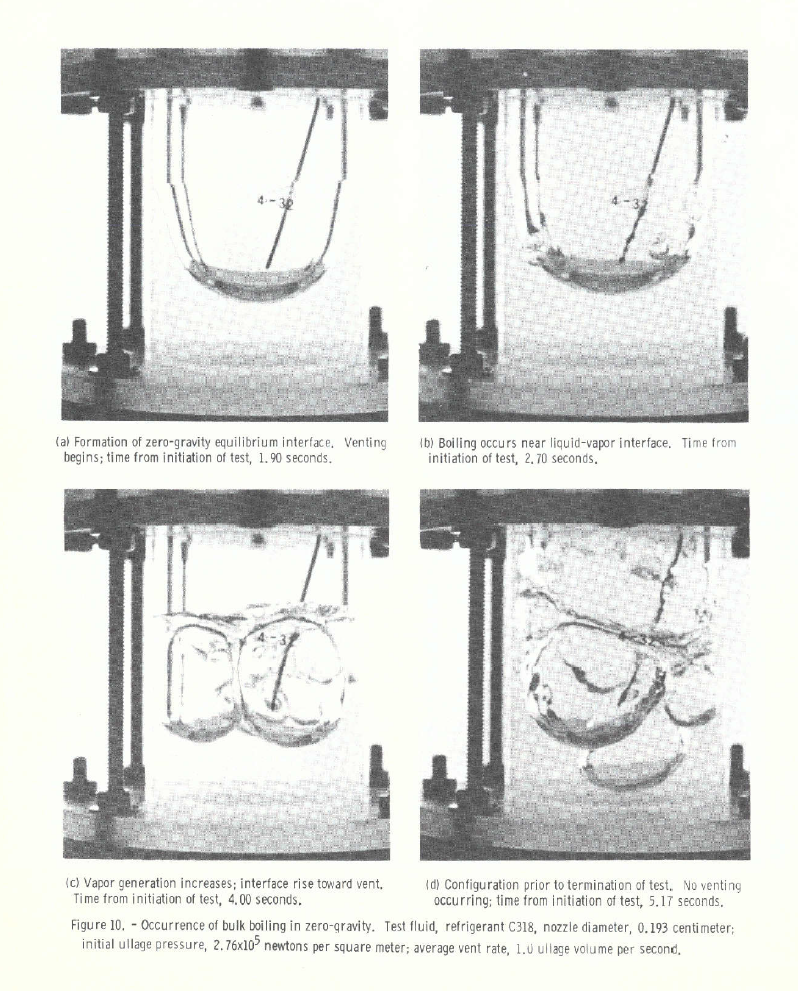
\includegraphics[width=0.95\textwidth]{images/labus_1p0_ullage_per_s.png}
\caption{Occurrence of bulk boiling in zero-gravity at high vent rate ($\sim$1.0 ullage volume per second). Test fluid: Refrigerant C318; initial ullage pressure: $2.76\times10^5$ N/m$^2$. (a) Zero-gravity interface formation; (b) boiling near interface; (c) increasing vapor generation and interface rise; (d) final configuration prior to vent termination.}
\label{fig:labus_1p0}
\end{figure}

\begin{figure}[htbp]
\centering
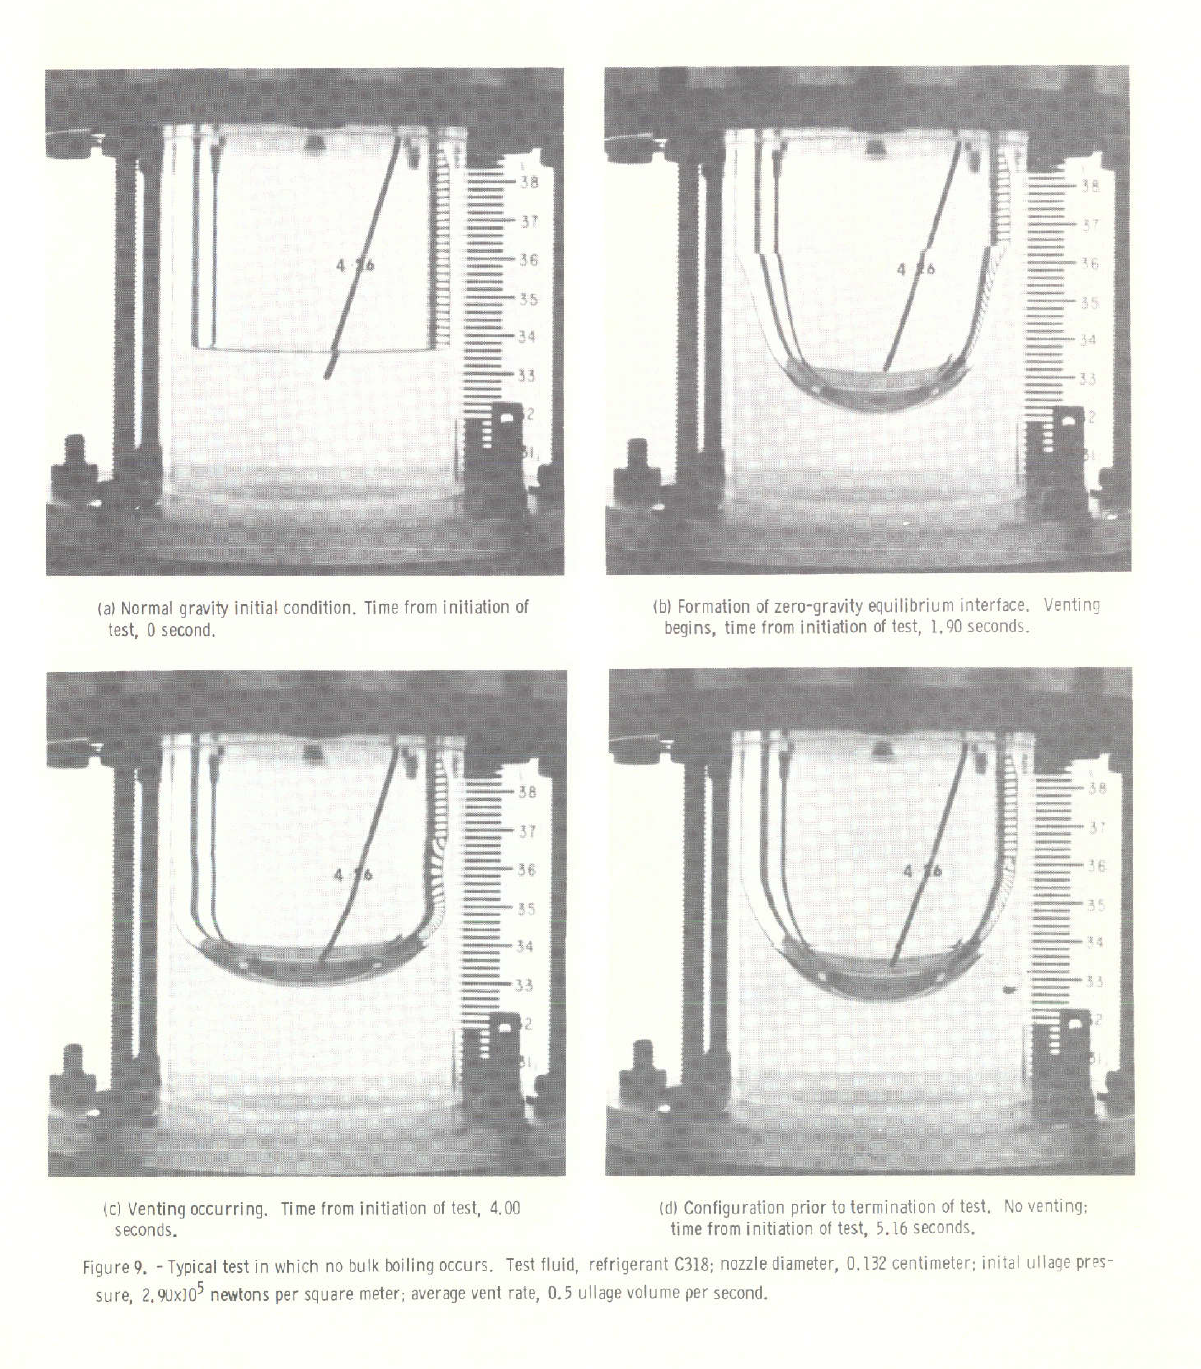
\includegraphics[width=0.95\textwidth]{images/labus_0p5_ullage_per_s.png}
\caption{Typical test showing no bulk boiling at lower vent rate (0.5 ullage volume per second). Test fluid: Refrigerant C318; initial ullage pressure: $2.90\times10^5$ N/m$^2$. (a) Normal-gravity initial condition; (b) zero-gravity interface formation; (c) venting in progress; (d) final configuration prior to vent termination.}
\label{fig:labus_0p5}
\end{figure}


\subsection{The Saturn S-IVB AS-203 Flight Experiment}
The most comprehensive in-orbit data on cryogenic liquid behavior during venting were obtained during the Saturn S-IVB AS-203 mission launched on 5 July 1966 \cite{AS203_1970}. The experiment featured three distinct rapid depressurization sequences of the liquid hydrogen tank, executed with both the Continuous Vent System (CVS) and the Non-Propulsive Vent (NPV) system. These controlled pressure reductions of several psi occurred while the vehicle remained in a low-gravity coast environment ($\sim10^{-4}$ to $10^{-5}$\,g).

\begin{figure}[htbp]
\centering
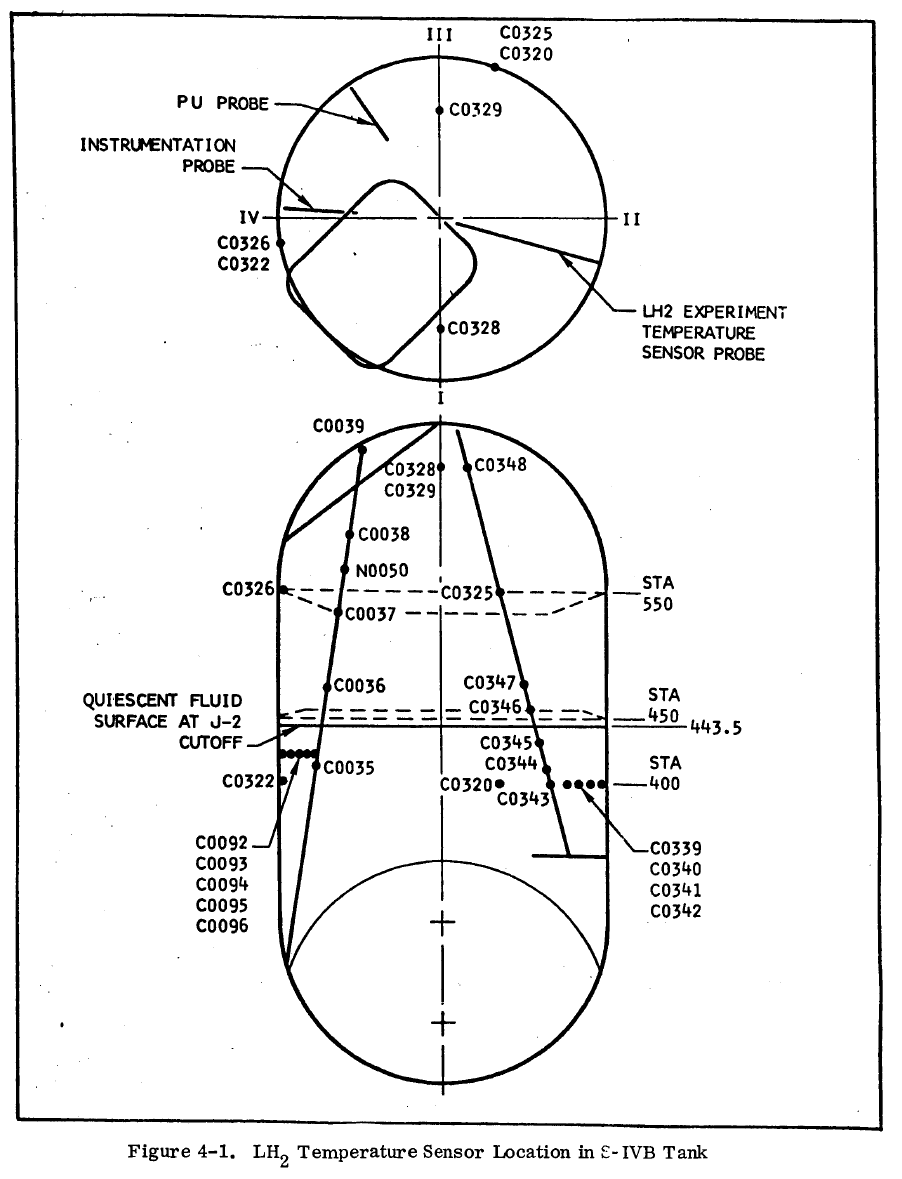
\includegraphics[width=0.95\textwidth]{images/saturn_temp_sensors_location.png}
\caption{Locations of temperature sensors and liquid-vapor detectors in the S-IVB liquid hydrogen tank during the AS-203 experiment \cite{AS203_1970}.}
\label{fig:as203_sensors}
\end{figure}

\begin{figure}[htbp]
\centering
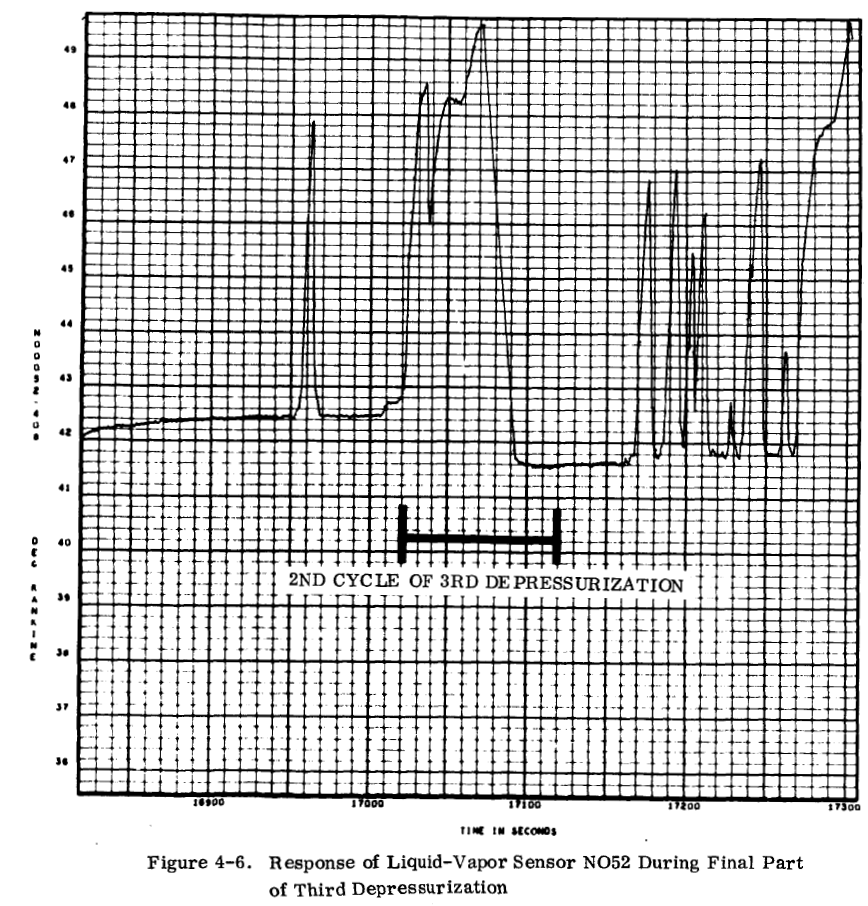
\includegraphics[width=0.95\textwidth]{images/saturn_temp_sensor_wetting.png}
\caption{Response of liquid-vapor sensor N052 during the third depressurization, confirming upward motion of the liquid-vapor interface \cite{AS203_1970}.}
\label{fig:as203_n052}
\end{figure}

\begin{figure}[htbp]
\centering
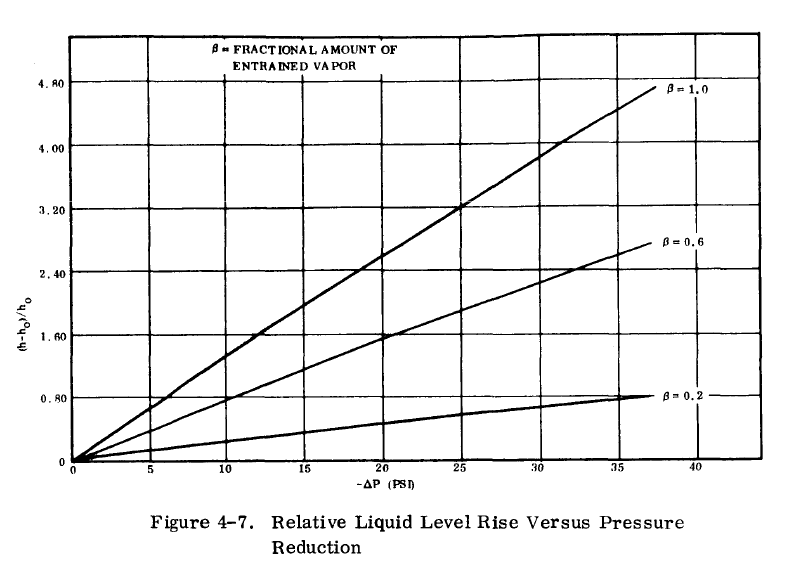
\includegraphics[width=0.95\textwidth]{images/saturn_liqlev_vs_pressure.png}
\caption{Measured relative liquid level rise versus pressure reduction during AS-203 venting events \cite{AS203_1970}.}
\label{fig:as203_llr_vs_dp}
\end{figure}

The S-IVB LH$_2$ tank was instrumented with an extensive array of temperature diodes positioned at multiple axial stations along with dedicated liquid-vapor point sensors. Of particular importance was liquid-vapor sensor N052 (also denoted NO52), which was located at the same axial station as temperature diode C0347, positioned slightly above the nominal liquid-vapor interface (approximately 43\,\% fill level at station 438). Sensor N052 was a variable-resistance type device similar to those used on the Centaur vehicle. It proved to be the only liquid-vapor sensor that operated reliably; its wetting and drying indications agreed closely with the temperature response of the co-located diode C0347. The remaining liquid-vapor sensors exhibited anomalous behavior, apparently trapping liquid once wetted and thereby producing erroneous persistent wet indications.

During the second and third depressurization events, sensor N052—initially residing in the ullage—registered a transition to liquid contact, providing direct evidence of substantial upward displacement of the liquid-vapor interface. Temperature diode readings near the initial interface revealed regions of superheated liquid followed by rapid cooling associated with boiling onset. Quantitative analysis of the flight data demonstrated that the observed liquid level rise substantially exceeded that attributable to simple flashing or volumetric expansion alone, scaling strongly with both the magnitude and rate of pressure reduction (Figure~\ref{fig:as203_llr_vs_dp}).

These unique low-gravity venting observations established that vapor generation within the thermal boundary layer along the wetted tank sidewall, together with bulk flashing, produced significant bulk liquid displacement. The AS-203 flight data therefore provided the definitive validation benchmark and served as the primary motivation for the development of the original LIQLEV analytical boundary-layer model, which explicitly accounts for wall-driven boil-off and its contribution to interface rise.

\subsection{Development of the Original LIQLEV Model}
Following the AS-203 flight, the LIQLEV (Liquid Level) boundary-layer model was developed in Fortran to predict the contribution of wall boundary-layer boil-off to bulk liquid displacement. The model, fully documented in Appendix B of NASA CR-109847, focused on vapor generation within a thin thermal boundary layer along the wetted tank sidewall and its effect on the upward motion of the liquid-vapor interface.

\begin{figure}[htbp]
\centering
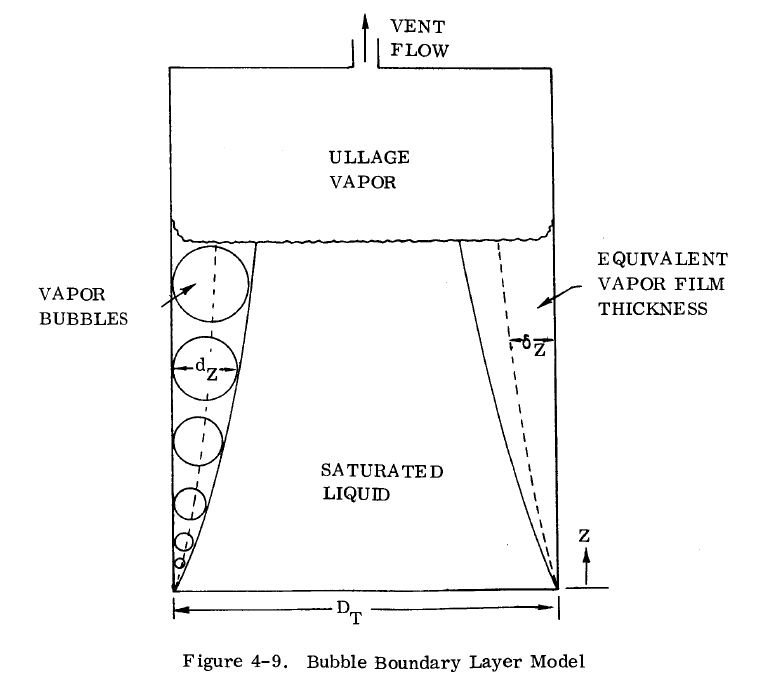
\includegraphics[width=0.95\textwidth]{images/saturn_boundary_layer_model.png}
\caption{Bubble boundary-layer model developed for the AS-203 liquid hydrogen tank \cite{AS203_1970}. The model treats vapor generation within a thin thermal boundary layer along the wetted sidewall, with bubbles contributing to bulk liquid displacement.}
\label{fig:liqlev_boundary_layer}
\end{figure}

As illustrated in Figure~\ref{fig:liqlev_boundary_layer}, the model treats the sidewall as a surface on which a growing vapor film forms; bubbles nucleate, grow, and detach within this film, displacing liquid and raising the interface. The governing physics are expressed through unsteady mass and energy balances on differential elements of the boundary layer (Figure~\ref{fig:liqlev_mass_balance}), yielding the instantaneous vapor volume $V_{\rm BL}(t)$ and the resulting interface velocity
\[
\frac{dh}{dt} = \frac{1}{A_c}\frac{dV_{\rm BL}}{dt},
\]
where $A_c$ is the tank cross-sectional area. Parametric studies examined the sensitivity of liquid level rise to vent rate, tank diameter, gravity level, and bubble spacing.

\begin{figure}[htbp]
\centering
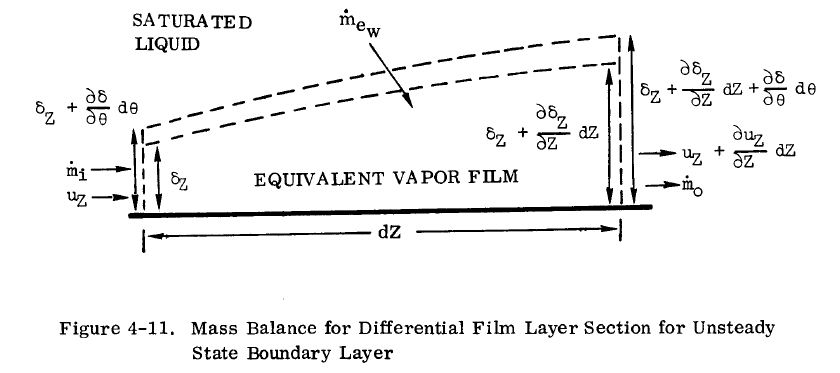
\includegraphics[width=0.95\textwidth]{images/saturn_mass_balance.png}
\caption{Mass balance for a differential element of the unsteady thermal boundary layer in the original LIQLEV model \cite{AS203_1970}}
\label{fig:liqlev_mass_balance}
\end{figure}

In recent years, Moran \cite{MoranVBA} adapted the original Fortran code into an Excel Visual Basic for Applications (VBA) environment to support the Human Landing System (HLS) program. This adaptation required meticulous line-by-line debugging of the legacy source code from the poorly scanned NASA CR-109847 reports. Moran’s implementation successfully replicated the AS-203 flight conditions, replaced outdated hydrogen property curve fits with initial calls to the CoolProp library, and introduced a dynamic ratio $\epsilon$ representing the proportion of boil-off generated in the wall boundary layer relative to the free surface. This ratio was made dependent on the wetted wall area and interface area.

Although functional, the VBA version was limited by its sequential execution and tight integration within Excel, making it unsuitable for large-scale parametric studies and modern computational workflows.

\subsection{Modernization of the LIQLEV Model}
To address the limitations of the VBA implementation and fulfill the requirements of the FY25 Drop Tower LLR Study, the LIQLEV model was completely reimplemented in Python as two tightly integrated modules: a core transient solver (\texttt{liqlev\_simulation}) and a high-throughput 2D geometry sweep driver (\texttt{liqlev\_sweep.py}). This modernization provides several critical advancements, including high-accuracy thermodynamic property evaluation, support for arbitrary time-dependent vent profiles, robust numerical safeguards, and efficient parallel processing for thousands of configurations.

\subsubsection{Thermodynamic Integration via CoolProp}
The original VBA code relied on localized, hardcoded property lookups and outdated curve fits (primarily for hydrogen), which severely limited flexibility for other cryogens and broad pressure regimes. The Python version integrates the open-source \texttt{CoolProp} library \cite{CoolProp} to provide consistent, high-accuracy real-fluid properties for Nitrogen, Hydrogen, Oxygen, and Methane across any pressure range.

Dedicated wrapper functions (\texttt{Cpsat}, \texttt{DensitySat}, \texttt{EnthalpySat}, \texttt{LHoV}, \texttt{Tsat}, \texttt{Psat}) evaluate saturation properties at every time step using direct \texttt{PropsSI} calls. The critical saturation-curve slope $\left(\frac{dP}{dT}\right)_{\rm sat}$, essential for depressurization and flashing calculations, is computed dynamically via a central finite-difference scheme with $\Delta P = 0.2$\,kPa to ensure numerical stability near the critical point. Hydrogen retains its original high-fidelity polynomials (valid for 10--50\,psia) for exact replication of AS-203 conditions, while all other fluids use full CoolProp evaluations. Unit conversions (psia $\leftrightarrow$ kPa, Rankine $\leftrightarrow$ K, lbm/ft³ $\leftrightarrow$ kg/m³) are handled transparently within the wrappers. This architecture eliminates hardcoded tables, supports any cryogen, and enables seamless extension to future fluids.

\subsubsection{Complex Vent Profile Implementation}
The legacy model supported only constant or linearly ramped vent rates. The Python implementation was upgraded to accept arbitrary time-dependent vent mass-flow-rate profiles supplied as paired arrays \texttt{tvmdot} (time points in s) and \texttt{xvmdot} (mass flow in lbm/s). Linear interpolation via the \texttt{sli} function is performed at every solver step.

For direct validation against the JAXA $30\,m^3$ LH$_2$ large-scale test \cite{tani2021pressure}, a high-fidelity piecewise profile was implemented in \texttt{get\_jaxa\_config}. The profile reproduces the rapid 0--15\,s stepped blowdown (four discrete steps from 0 to $\sim$0.065\,kg/s) followed by long-term decay to $\sim$0.010\,kg/s at 3600\,s, closely matching the experimental data in Figures 6 and 12 of the reference. This modification significantly improves the fidelity of predicted pressure decay (including the characteristic initial pressure recovery due to delayed bulk boiling), superheat evolution, boundary-layer vapor volume, and liquid level rise compared with the original fixed-rate assumption.

A new “bulk\_fake” epsilon mode was introduced to emulate distributed volumetric boiling in large tanks: setting $\epsilon \approx 50$ effectively scales the vapor-generating surface area by a factor of 50, reproducing the experimentally observed $\sim$6.85-inch interface displacement within the first few seconds.

\subsubsection{Multiprocessing for Parametric Sweeps}
The core requirement of the FY25 Drop Tower LLR Study is to execute large-scale parametric analyses varying tank geometry, initial fill level, vent flow rate, and gravity level. The dedicated script \texttt{liqlev\_sweep.py} utilizes Python’s \texttt{concurrent.futures.ProcessPoolExecutor} to run independent 2D geometry cases in parallel across all available CPU cores (dynamic worker count from SLURM environment or default 6).

For each diameter–height combination (50 diameters $\times$ 40 heights = 2000 geometries per vent rate), the full transient simulation is performed with an early-termination check that halts execution the instant $h_2 \ge h_{\rm tank}$ (with 0.9999 tolerance for floating-point safety). Liquid level rise values are extracted at fixed snapshots ($t=5$\,s, $t=20$\,s or end-of-run, and global peak) via \texttt{np.interp}. Results are stored as structured 2D NumPy grids and exported to Excel workbooks (one file per vent rate) with separate sheets for each snapshot, maximum rise, and overfill flag. Contour plots are automatically generated using \texttt{contourf} with hatched regions (\texttt{hatches=['XX']}) denoting lid-impingement geometries. A 2.0-inch target rise contour and baseline geometry marker are overlaid for rapid design-space visualization.

Additional solver robustness features include safeguards against zero driving force (\texttt{ak3} $\approx 0$), secant-method divide-by-zero protection, and extensive diagnostic outputs (superheat, vapor generation rate in kg/s, superficial vapor velocity, cumulative vapor mass, boundary-layer thickness, and instantaneous $\epsilon$). These enhancements collectively enable efficient evaluation of thousands of configurations while preserving full traceability and numerical stability.

The resulting computational framework provides a modern, extensible, and production-ready replacement for the legacy code, directly supporting the experimental test matrix optimization described in Section~\ref{sec:exp_design_parameter_sweeps}.

The modernized LIQLEV framework retains the original one-dimensional piston-like displacement assumption, whereby all vapor generated (boundary-layer plus flashing) is treated as uniformly distributed across the tank cross-section. The bulk\_fake mode provides a practical engineering approximation for large-scale tanks in which distributed volumetric boiling dominates; future work will replace this with an explicit bulk-liquid boiling source term while preserving the wall boundary-layer formulation.

\section{Experimental Design and Parameter Sweeps}
\label{sec:exp_design_parameter_sweeps}

The modernized LIQLEV framework was used to identify optimal test conditions for three NASA reduced-gravity facilities. The objective was to ensure that the maximum liquid-vapor interface rise could be fully captured within each facility’s available test duration while preventing lid impingement.

The candidate platforms were:

\begin{itemize}
    \item \textbf{NASA GRC 2.2-Second Drop Tower:} $\sim10^{-5}$\,g quality with a highly constrained 2.2\,s test window, requiring rapid interface dynamics to observe the initial transient.
    \item \textbf{NASA GRC 5-Second Zero-Gravity Facility:} $\sim10^{-5}$\,g quality, offering sufficient duration for slower boundary-layer growth and attainment of the peak liquid level rise.
    \item \textbf{Parabolic Flight Campaigns:} $\sim$17\,s of reduced gravity ($\sim10^{-2}$ to $10^{-3}$\,g with typical g-jitter), permitting observation of longer-term thermodynamic stabilization and quasi-steady boiling.
\end{itemize}

Facility-specific gravity histories are incorporated through a custom \texttt{gravity\_function} callback. For the 5-second zero-gravity facility, accelerometer data recorded during prior drop-tower tests (normalized time and axial acceleration) are converted to ft/s². A constant hold value is appended beyond the last measured data point, deliberately allowing each simulation to be extended well beyond the nominal 5\,s duration (up to 20\,s). 

This extension was essential to determine whether the true maximum liquid level rise is attained \textit{within} the available 5\,s microgravity window or only later. By comparing the time of peak rise against the rigid facility limit, optimal tank geometries, fill fractions, and vent rates could be identified that fully capture the complete transient---from initial meniscus reorientation through sustained boundary-layer-driven rise---before the end of the test window, while strictly avoiding lid impingement.

\subsection{Governing Parameters}
The parameter sweep systematically quantified the coupled effects of geometry, thermodynamics, venting, and gravity level on transient liquid level rise (LLR). The following variables were varied across the full matrix:

\begin{enumerate}
    \item \textbf{Tank Geometries and Aspect Ratios ($L/D$):} The primary parametric grid consisted of 50 diameter values (0.2--1.0\,ft) and 40 height values (0.3--2.5\,ft), yielding 2000 unique geometries per vent rate and spanning aspect ratios from $L/D \approx 2$ to over 12. Targeted smaller-scale configurations were also evaluated, including Skinner tanks with diameters ranging from 0.2 to 0.3\,ft at a fixed height of 2\,ft, as well as miniature cylindrical tanks matching the dimensions used in the Labus et al. experiments (6\,cm diameter $\times$ 10\,cm height).

    \item \textbf{Gravity Levels:} $10^{-3}$\,g, $10^{-4}$\,g, and $10^{-5}$\,g, bracketing the operational envelopes of all three facilities. Each level was implemented either as a constant value or via piecewise \texttt{gravity\_function} callbacks.

    \item \textbf{Initial Fill Levels:} Liquid volume fractions from 20\,\% to 80\,\%. Detailed matrices typically spanned 25--65\,\% to provide adequate optical visibility while maintaining sufficient margin against lid impingement.

    \item \textbf{Vent Flow Rates:} Constant rates scaled according to tank size. For tanks with diameters of 0.2\,ft and larger (including the 2\,ft height Skinner series), four discrete rates between 0.003 and 0.006\,lbm/s were selected. These rates produced controlled depressurization rates that generated measurable liquid level rise while keeping the interface safely below the tank lid for the chosen initial fill fractions. Proportionally smaller vent rates were applied to the miniature Labus-scale tanks (6\,cm diameter $\times$ 10\,cm height) to maintain comparable thermodynamic behavior across scales.
\end{enumerate}

Nitrogen was employed as the baseline fluid for the primary geometric sweeps because it is the planned working fluid for the actual drop-tower experiments. This selection enables rapid computation and provides direct correlation with the planned hardware, while offering excellent optical transparency for high-speed imaging. Separate validation runs using hydrogen were performed against the JAXA $30\,m^3$ LH$_2$ large-scale test data to ensure model fidelity for flight-relevant cryogens.

\subsection{Optimization Criteria}
The optimization process identified tank geometries, initial fill fractions, and vent rates that maximize scientific return within each facility’s rigid time constraint while strictly preventing liquid impingement on the tank lid. Scientific return was defined as the ability to optically capture the complete liquid-vapor interface transient---from rapid meniscus reorientation through sustained boundary-layer-driven rise and eventual stabilization---under high-quality microgravity conditions.

The two primary optimization criteria were:
\begin{itemize}
    \item The peak liquid-vapor interface height must be attained \textit{within} the available reduced-gravity duration and must produce an optically measurable rise of at least 2 inches. This minimum rise threshold ensures the thermodynamic signal substantially exceeds residual g-jitter and imaging-system noise, enabling clear and unambiguous capture of the complete transient response with high-speed imaging.
    \item The initial fill fraction must be constrained such that cumulative vapor generation (from both the free interface and wall thermal boundary layer) and the associated volumetric swelling keep the interface below the tank ceiling ($Z_{\rm int}(t) < Z_{\rm tank}$ for all $t \leq t_{\rm facility}$).
\end{itemize}

In microgravity the liquid-vapor interface rapidly transitions from a flat 1$g$ surface to a highly curved meniscus whose equilibrium shape is governed by the contact angle and the minimization of surface energy. Superimposed venting drives upward bulk motion through distributed bubble generation and displacement within the liquid column. 

The Python implementation explicitly tracks the instantaneous interface location $Z_{\rm int}(t)$ (denoted internally as \texttt{h2} or \texttt{zht2}) via the discrete relation
\[
Z_{\rm int}(t) = Z_{\rm int}(t-\Delta t) + \frac{\Delta V_{\rm BL} + \Delta m_{\rm liq}/\rho_{\rm liq}}{A_c}\,\Delta t,
\]
where $\Delta V_{\rm BL}$ is the incremental vapor volume generated in the wall thermal boundary layer, $\Delta m_{\rm liq}$ is the mass of liquid flashed to vapor, $\rho_{\rm liq}$ is the saturated liquid density, and $A_c = \pi D^2/4$ is the tank cross-sectional area. This formulation embodies the one-dimensional piston-like displacement assumption central to the original LIQLEV boundary-layer model.

An early-termination flag halts each simulation the instant $Z_{\rm int} \ge Z_{\rm tank}$, records the overfill condition, and excludes that geometry from further analysis. Liquid level rise values are extracted at multiple strategically chosen snapshots ($t=5$\,s, $t=20$\,s or end-of-run, and the global peak) via linear interpolation. These multi-time results, together with the overfill flag, are exported to structured .xlsx grids. This framework enables automated contour plotting with hatched regions denoting invalid (lid-impingement) configurations, greatly facilitating rapid and informed selection of viable experimental test articles.

\section{Results and Discussion}
\label{sec:results_discussion}

Extensive parametric simulations were performed with the modernized LIQLEV model to characterize transient liquid level rise (LLR) across the three target reduced-gravity facilities. Nitrogen was employed as the baseline working fluid for the large-scale geometric sweeps, which encompassed more than 2000 unique tank configurations per vent rate. Dedicated hydrogen cases were executed separately to provide direct validation against the JAXA $30\,m^3$ LH$_2$ large-scale experiment. All computed results are fully consistent with the time-history plots, contour maps, and sensitivity studies compiled in the Cryo Vent Study Phase Summary document.


% \subsection{Influence of Gravity Level on Liquid Level Rise}

% Background acceleration exhibits a strong non-linear inverse relationship with maximum liquid level rise. At $10^{-3}$\,g, residual buoyancy forces promote partial vapor bubble stratification and departure, limiting the residence time of vapor within the bulk liquid column. As gravity decreases to $10^{-5}$\,g (representative of the NASA GRC drop towers), bubble departure diameter increases substantially while the relative rise velocity of bubbles with respect to the liquid bulk approaches zero. Vapor generated in the wall boundary layer and at the interface therefore remains entrained, acting effectively as distributed void volume that inflates the liquid column.

% This mechanism is quantified directly in the model through the boundary-layer vapor volume $V_{\rm BL}$ and the instantaneous interface velocity:
% \[
% \frac{dh}{dt} = \frac{1}{A_c}\left(\frac{dV_{\rm BL}}{dt} + \frac{1}{\rho_l}\frac{dm_l}{dt}\right),
% \]
% where $A_c = \pi D^2/4$ is the tank cross-sectional area. Consequently, the most aggressive LLR occurs at the lowest gravity levels (Figure~\ref{fig:key_findings}).

% % \begin{figure}[htbp]
% % \centering
% % \includegraphics[width=0.95\textwidth]{figures/key_findings_8-28-25.pdf}
% % \caption{Summary of facility performance and liquid level rise behavior across gravity levels and test durations (Cryo Vent Study Phase Summary, 8/28/25).}
% % \label{fig:key_findings}
% % \end{figure}

% Variable-gravity parabolic-flight profiles (low-g plateaus of 0.08\,g or 0.01\,g) were also evaluated and confirmed that the full transient can be captured during the low-g portion, yielding rises of 0.5--2+ inches depending on vent rate and fill level (Figure~\ref{fig:variable_gravity}). In contrast, the 2.2 s and 5.5 s drop-tower environments, although achieving the same ultra-low gravity quality, do not provide sufficient duration for the interface to reach its asymptotic maximum; higher vent rates are therefore required to generate a measurable rise within the rigid time window.

% % \begin{figure}[htbp]
% % \centering
% % \includegraphics[width=0.95\textwidth]{figures/variable_gravity_parabolic.pdf}
% % \caption{Gravity profiles and corresponding liquid level rise for parabolic-flight variable-gravity cases (0.08 g and 0.01 g low-g plateaus).}
% % \label{fig:variable_gravity}
% % \end{figure}

\subsection{Influence of Gravity Level on Liquid Level Rise}
Background acceleration exhibits a strong non-linear inverse relationship with maximum liquid level rise. At $10^{-3}$\,g, residual buoyancy forces promote partial vapor bubble stratification and departure, limiting the residence time of vapor within the bulk liquid column. As gravity decreases to $10^{-5}$\,g (representative of the NASA GRC drop towers), bubble departure diameter increases substantially while the relative rise velocity of bubbles with respect to the liquid bulk approaches zero. Vapor generated in the wall boundary layer and at the interface therefore remains entrained, acting effectively as distributed void volume that inflates the liquid column.

This mechanism is quantified directly in the model through the boundary-layer vapor volume $V_{\rm BL}$ and the instantaneous interface velocity:
\[
\frac{dh}{dt} = \frac{1}{A_c}\left(\frac{dV_{\rm BL}}{dt} + \frac{1}{\rho_l}\frac{dm_l}{dt}\right),
\]
where $A_c = \pi D^2/4$ is the tank cross-sectional area. Consequently, the most aggressive liquid-level rise occurs at the lowest gravity levels.

Variable-gravity parabolic-flight profiles (low-g plateaus of 0.08\,g or 0.01\,g) were also evaluated and confirmed that the full transient can be captured during the low-g portion, yielding rises of 0.5--2+ inches depending on vent rate and fill level. In contrast, the 2.2-second and 5.5-second drop-tower environments, although achieving the same ultra-low gravity quality, do not provide sufficient duration for the interface to reach its asymptotic maximum; higher vent rates are therefore required to generate a measurable rise within the rigid time window.

%%%%%%%%%%%%%%%%%%%%%%%%%%%%%%%%%%%%%%%%%%%%%%%%%%


\subsection{Tank Aspect Ratio Effects (5-Second Facility)}
A broad parametric sweep was first executed across more than 2000 unique cylindrical geometries (50 diameters ranging from 0.19685\,ft to 1.0\,ft and 40 heights ranging from 0.328\,ft to 2.5\,ft) at $10^{-5}$\,g using the gravity profile extracted from prior NASA GRC drop-tower accelerometer data. Beyond the last measured point at 5\,s, the final acceleration value was held constant to enable realistic extrapolation for the 20\,s snapshot plots. The height-dependent epsilon formulation (dynamic ratio of wall boundary-layer vapor generation to free-surface generation) was used throughout all simulations.

From this large matrix, candidate tank dimensions were down-selected to satisfy two practical constraints derived from historical drop-tower hardware: a maximum diameter of approximately 1\,ft and a maximum height of 2\,ft (to fit inside existing drop capsules), while also encompassing the miniature scale used in the Labus et al.\ experiments (6\,cm diameter $\times$ 10\,cm height).

The primary analysis focused on identifying the optimal performance region in the contour plots — specifically the area lying between the red 2-inch measurable rise contour and the hatched overfill zones. The selection criterion was to identify tanks that produce an optically measurable rise (at least 2 inches, above the red contour) while remaining safely below the tank lid (outside the hatched overfill regions) for practical fill fractions and vent rates. Smaller-diameter tanks consistently delivered higher interface rise velocities because any incremental vapor volume $\Delta V_{\rm vapor}$ produces a larger interface displacement in the reduced cross-sectional area:
\[
\Delta Z = \frac{\Delta V_{\rm vapor}}{A_c}.
\]

Four representative geometries within this optimal band were examined in greater detail:
\begin{itemize}
    \item 1.0\,ft diameter $\times$ 2.0\,ft height ($L/D=2$)
    \item 0.75\,ft diameter $\times$ 2.0\,ft height ($L/D\approx2.67$)
    \item 0.5\,ft diameter $\times$ 2.0\,ft height ($L/D=4$)
    \item 0.3\,ft diameter $\times$ 2.0\,ft height ($L/D\approx6.67$)
\end{itemize}

Analysis of the contour plots revealed important trends. The 1.0\,ft-diameter tank proved too wide, providing excessive margin but insufficient rise within the 5-second window for most conditions. In contrast, the smaller-diameter Skinner-style tanks (0.2--0.3\,ft) offered much stronger rise signals. However, these narrower tanks often required slightly greater height to prevent liquid impingement, particularly at higher fill fractions. Increasing the initial fill fraction expanded the usable test region, with the best overall balance occurring near 50\,\% fill. At 75\,\% fill, however, the hatched overfill regions grew substantially, reducing the number of viable configurations.

The optimized test conditions were therefore identified near 50\,\% fill fraction and diameters between approximately 0.3\,ft and 0.4\,ft. Diameters in the 0.2--0.3\,ft range at 2\,ft height performed particularly well across the selected vent rates, falling optimally between the red measurable-rise contour and the hatched overfill regions.

These trends are illustrated in the tank-size sweep contour plots at 25\,\%, 50\,\%, and 75\,\% initial fill fraction for the four vent rates examined (Figures~\ref{fig:sweep_25_combined}, \ref{fig:sweep_50_combined}, \ref{fig:sweep_75_combined}). Each figure shows rise (inches) at $t=5$\,s, $t=20$\,s (or end-of-run), and global peak. The red contour marks the 2-inch measurable threshold, and hatched regions denote geometries that reach the tank lid within the 5-second window.

\begin{figure}[htbp]
\centering

\begin{subfigure}[b]{0.85\textwidth}
\centering
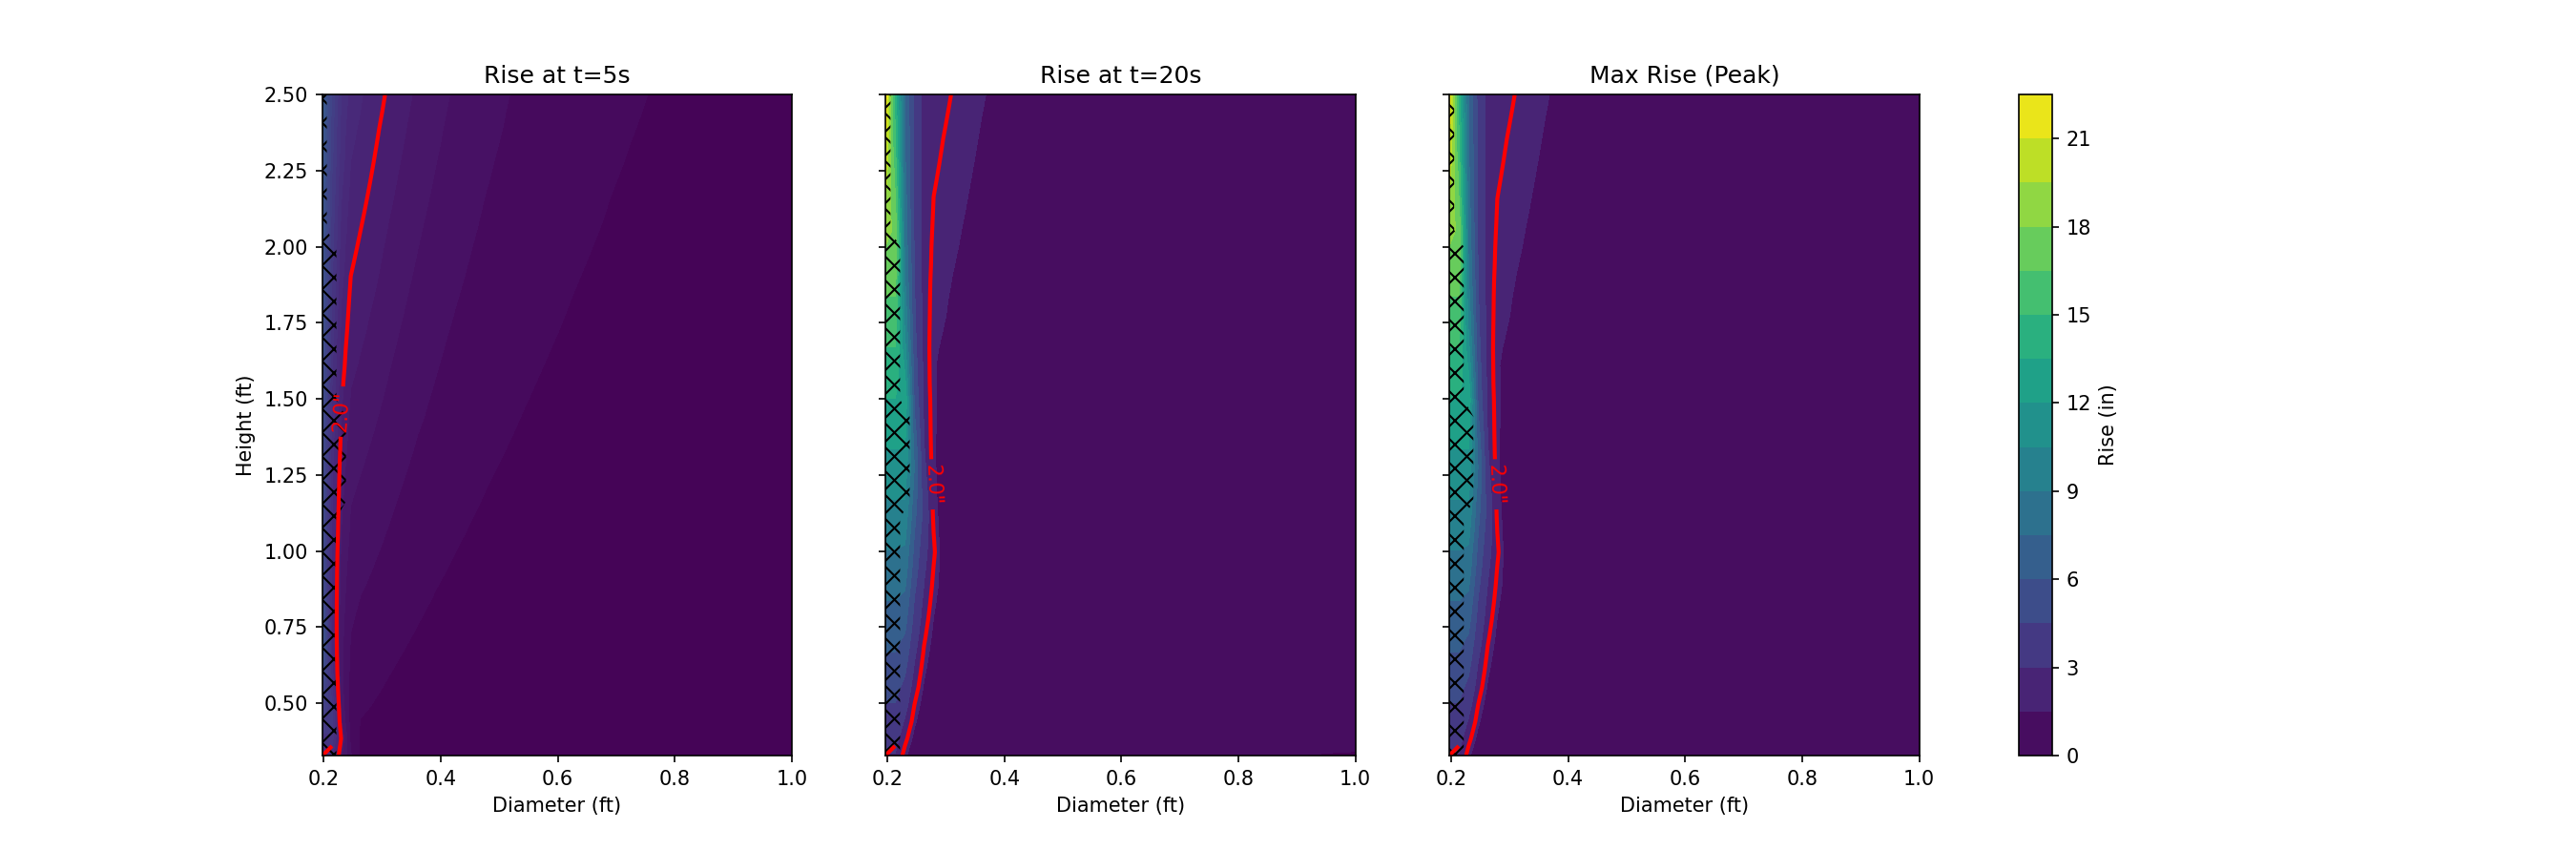
\includegraphics[width=\textwidth]{images/liqlev_25_fill_complete/plots_flow_0.003.png}
\caption{0.003\,lbm/s}
\end{subfigure}
\hspace{-0.6em}   % <-- allows gentle overlap
\begin{subfigure}[b]{0.85\textwidth}
\centering
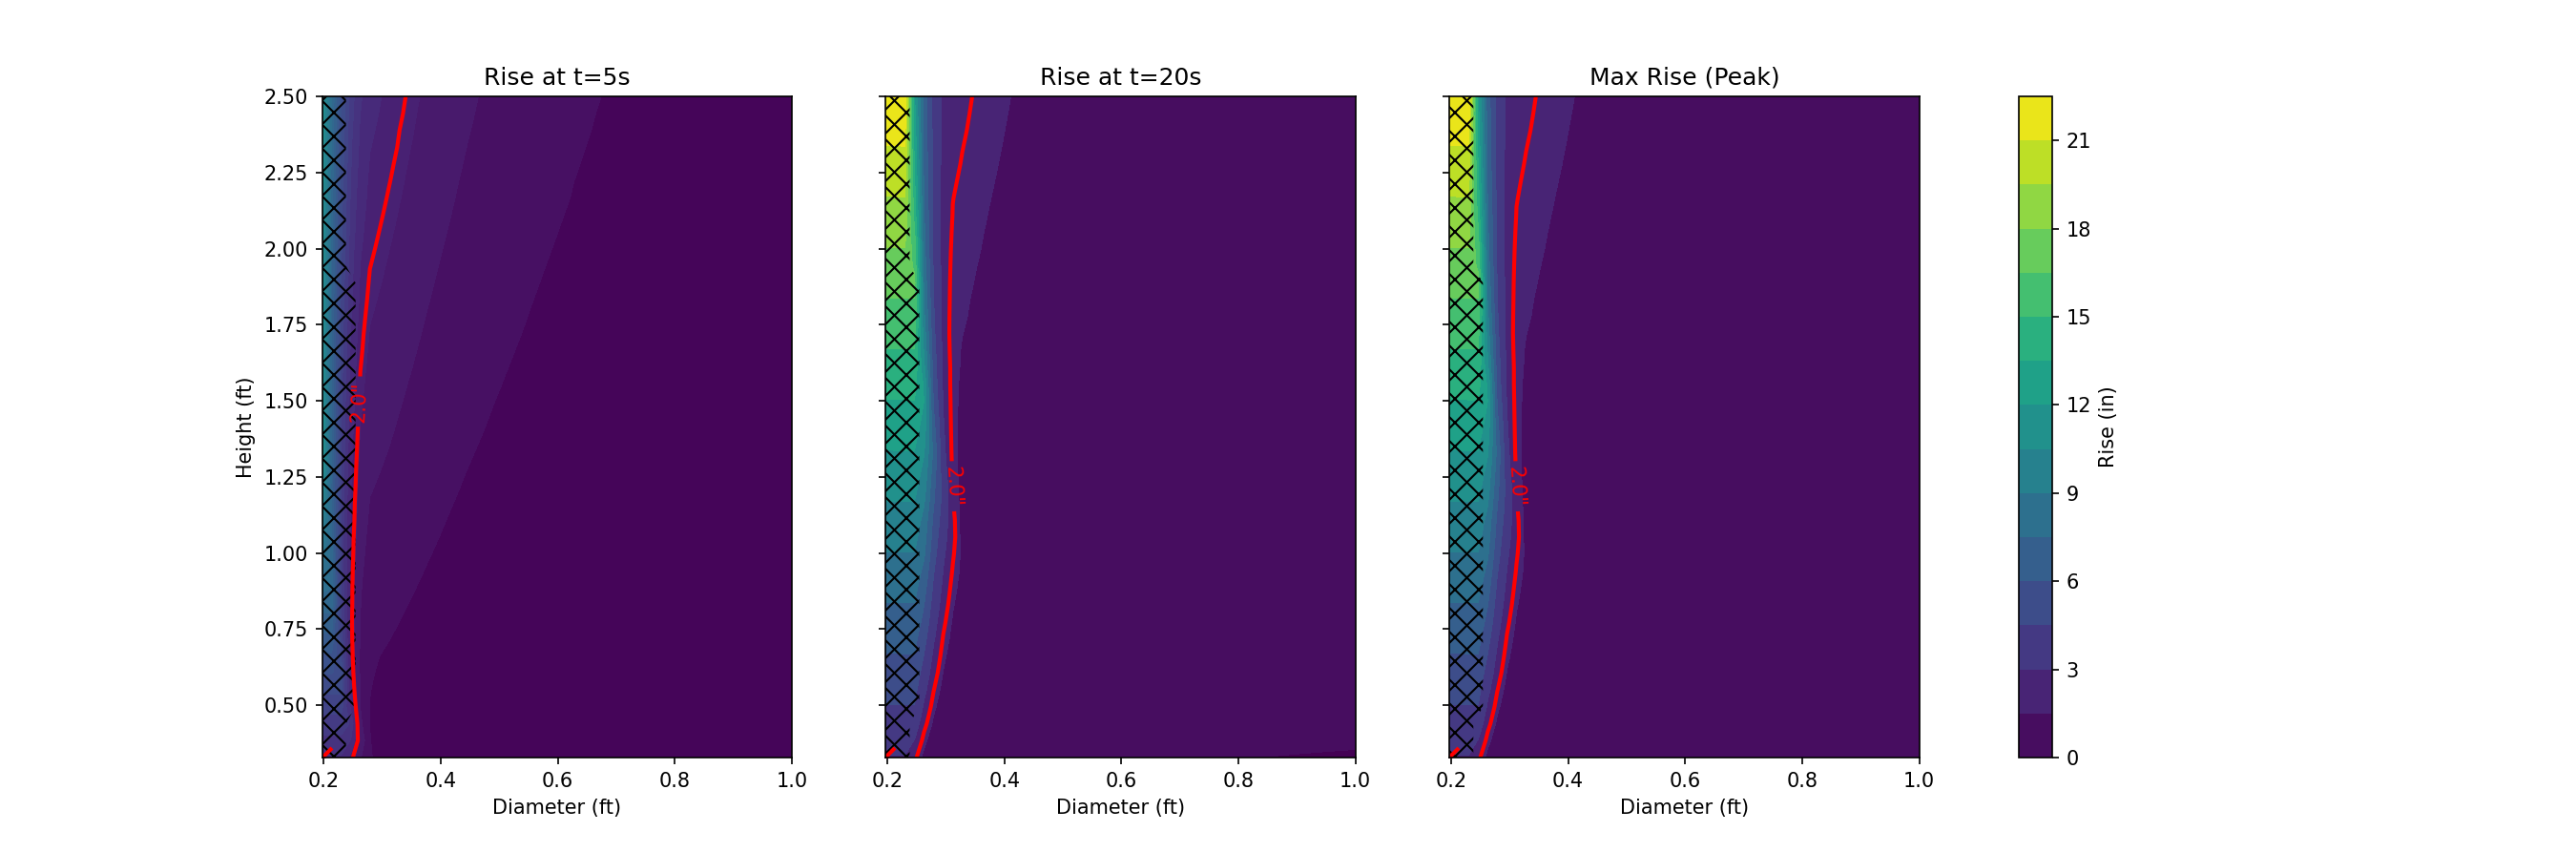
\includegraphics[width=\textwidth]{images/liqlev_25_fill_complete/plots_flow_0.004.png}
\caption{0.004\,lbm/s}
\end{subfigure}

\vspace{0.8em}    % <-- tighter vertical spacing

\begin{subfigure}[b]{0.85\textwidth}
\centering
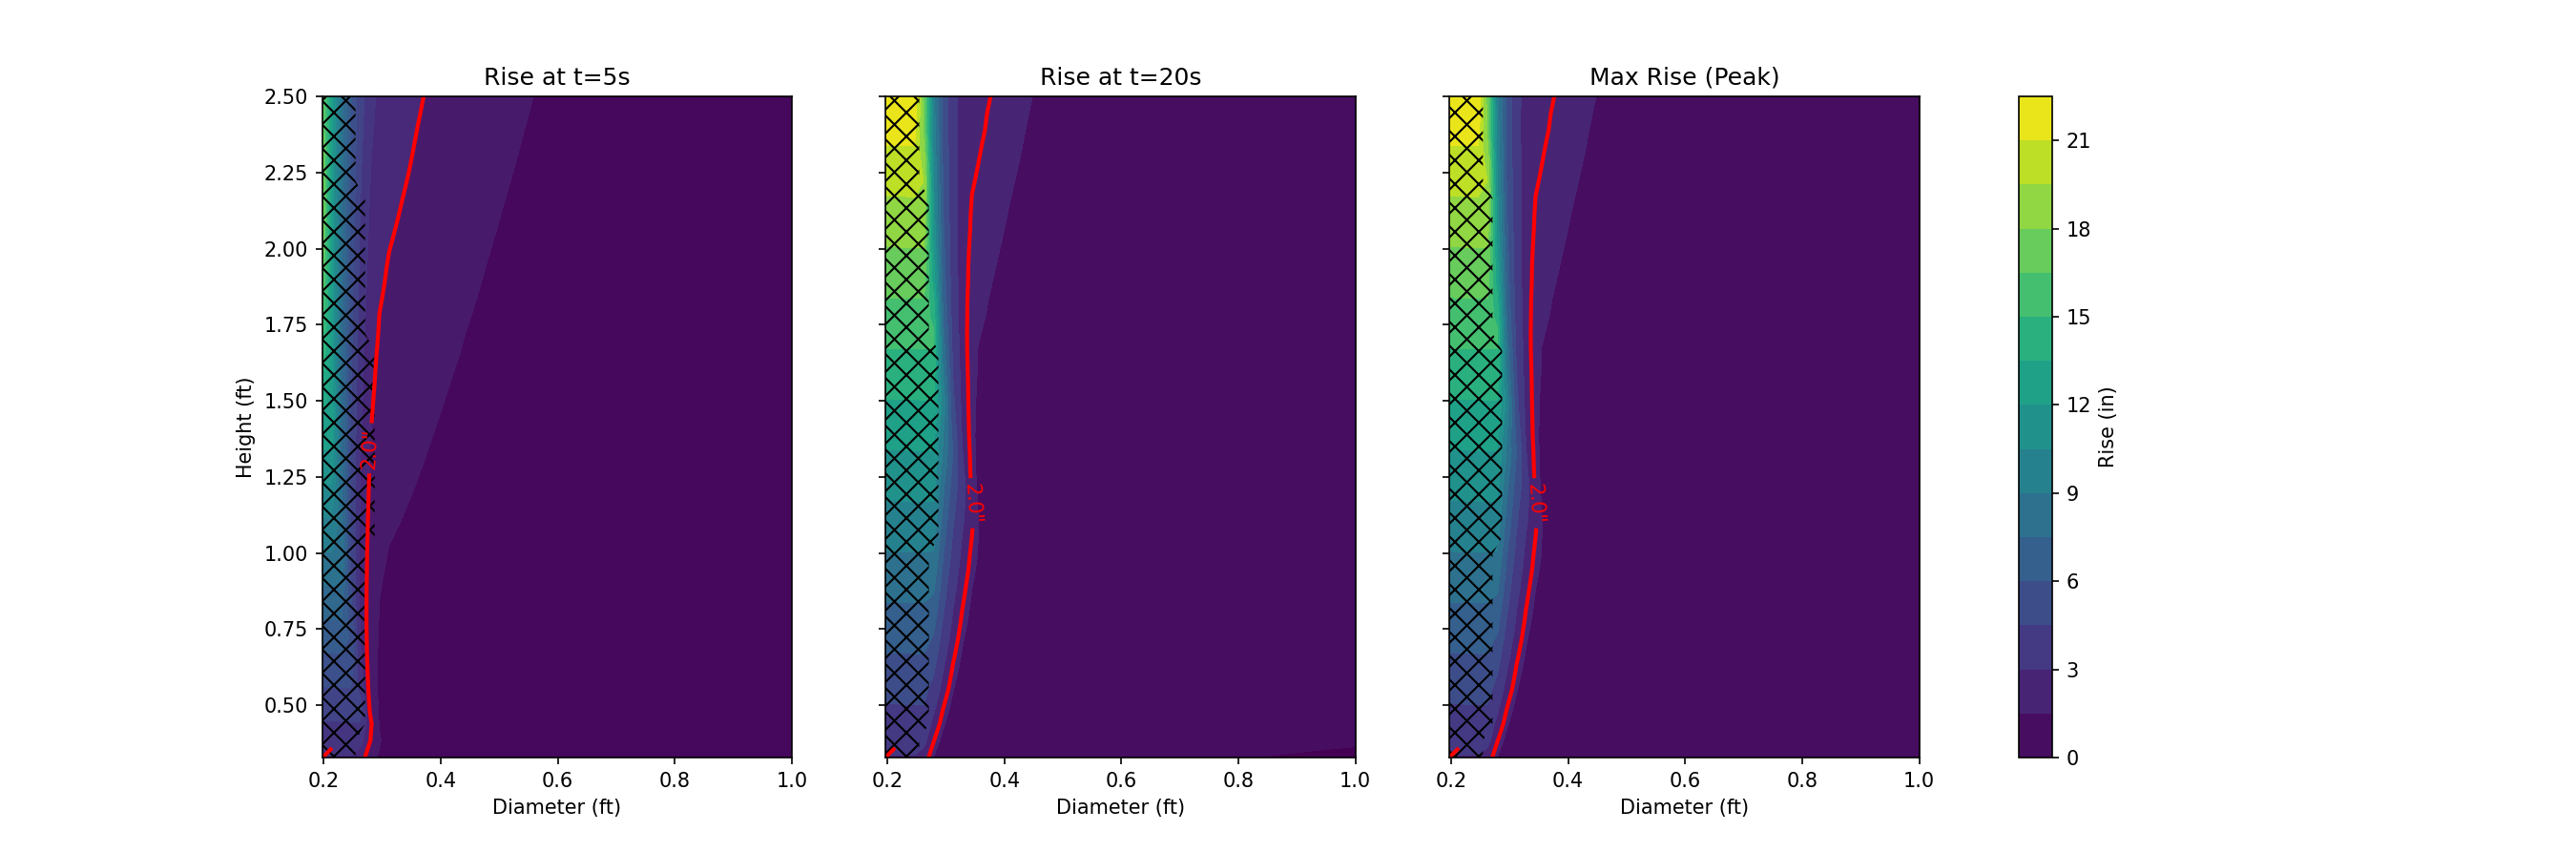
\includegraphics[width=\textwidth]{images/liqlev_25_fill_complete/plots_flow_0.005.png}
\caption{0.005\,lbm/s}
\end{subfigure}
\hspace{-0.6em}
\begin{subfigure}[b]{0.85\textwidth}
\centering
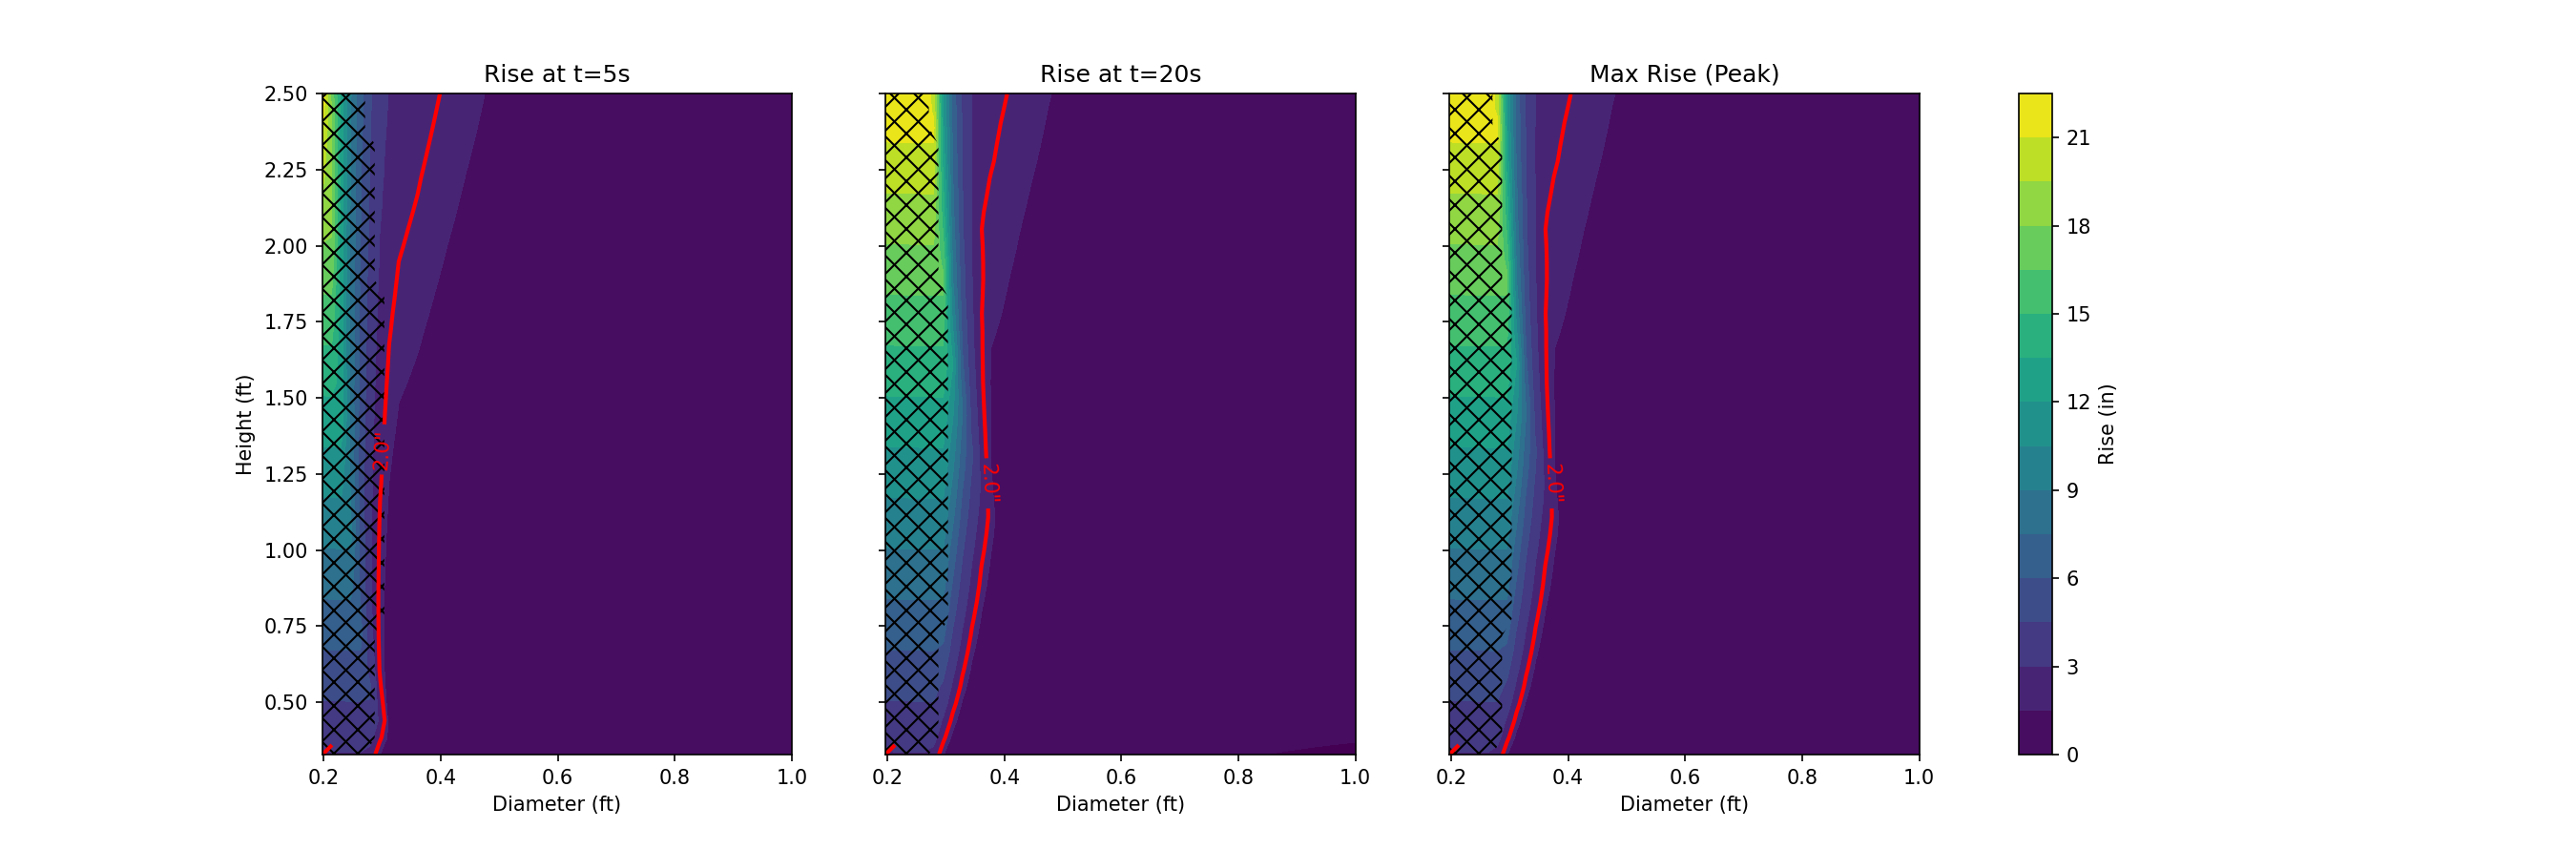
\includegraphics[width=\textwidth]{images/liqlev_25_fill_complete/plots_flow_0.006.png}
\caption{0.006\,lbm/s}
\end{subfigure}

\caption{Tank-size sweep results at 25\,\% initial fill fraction for the 5-second facility ($10^{-5}$\,g) across the four vent rates examined. Each panel shows rise (inches) at $t=5$\,s, $t=20$\,s (or end-of-run), and global peak. Red contour = 2-inch measurable threshold; hatched regions = lid impingement.}
\label{fig:sweep_25_combined}
\end{figure}

\begin{figure}[htbp]
\centering

\begin{subfigure}[b]{0.85\textwidth}
\centering
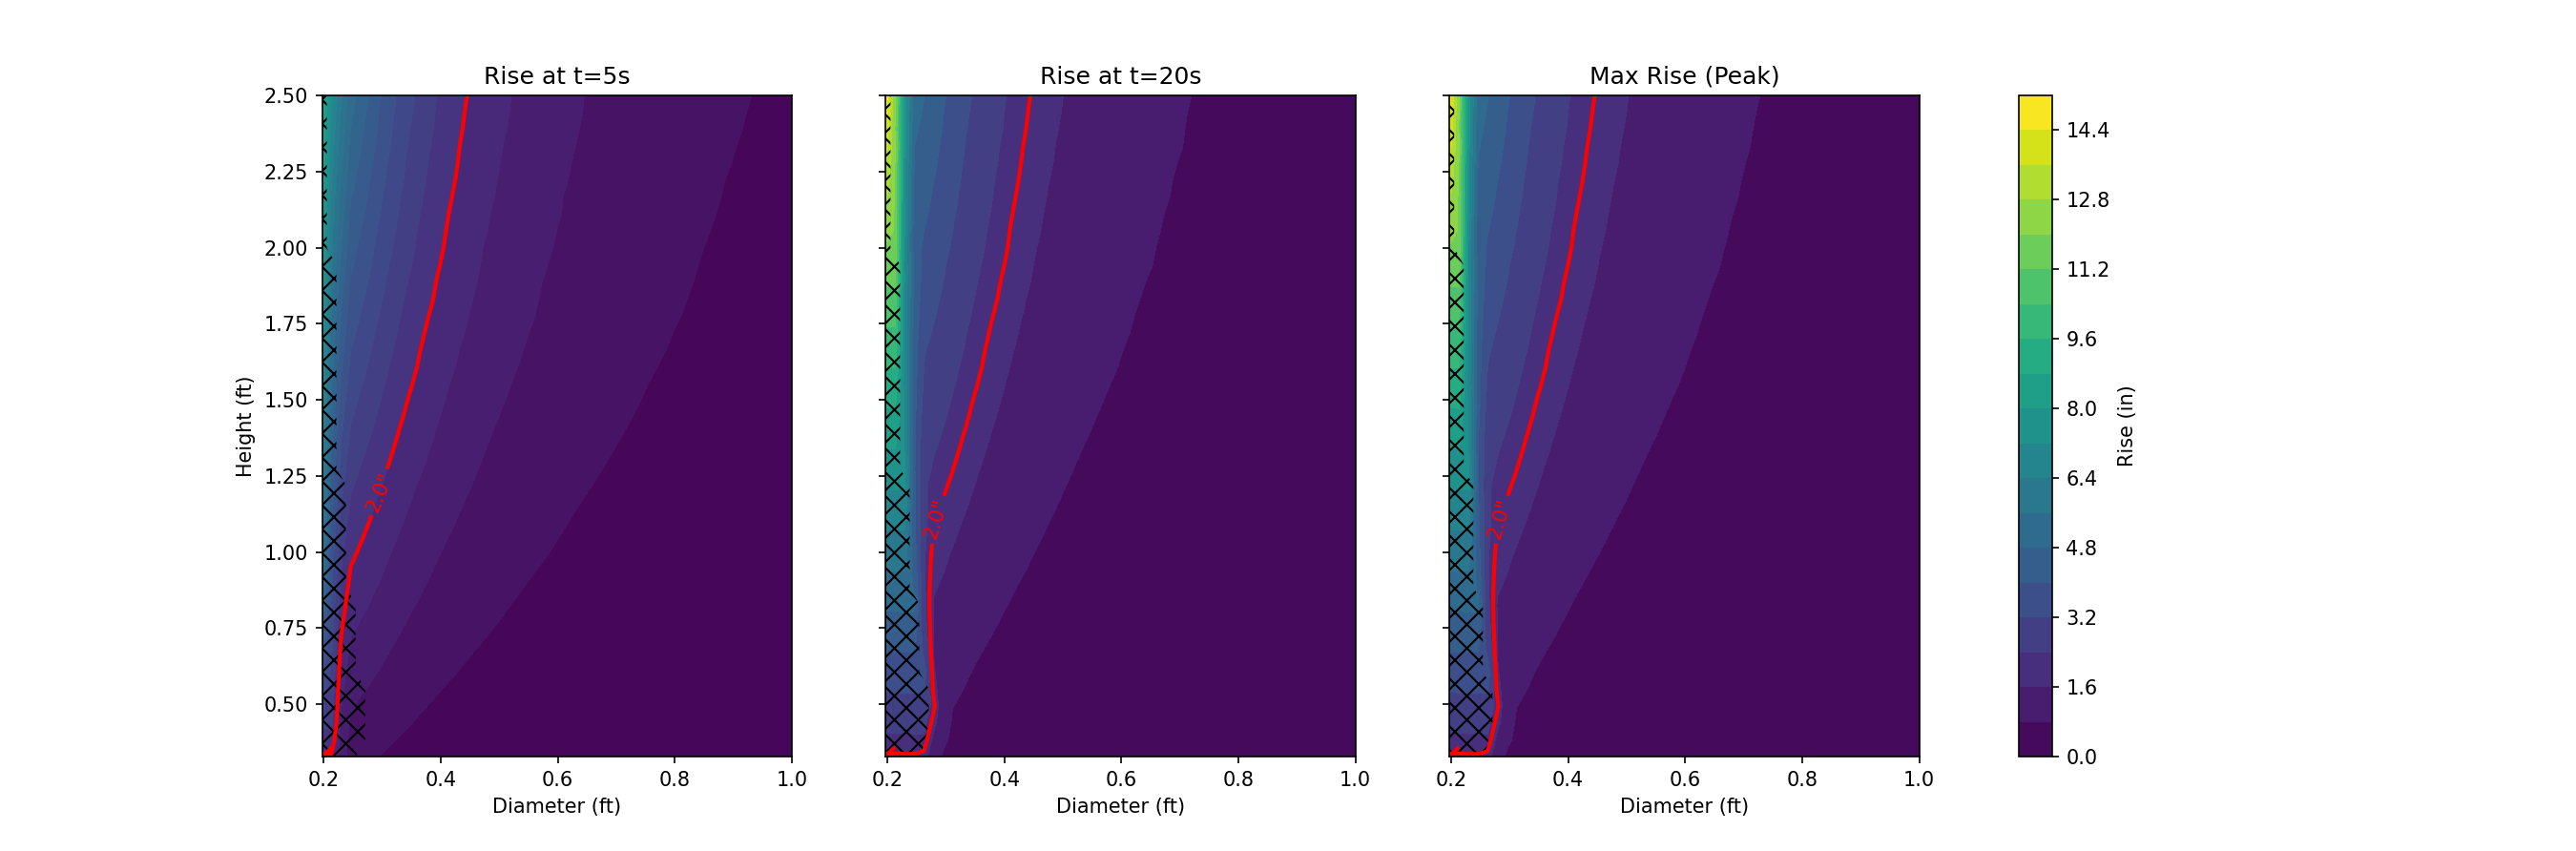
\includegraphics[width=\textwidth]{images/liqlev_50_fill_complete/plots_flow_0.003.png}
\caption{0.003\,lbm/s}
\end{subfigure}
\hspace{-0.6em}   % <-- allows gentle overlap
\begin{subfigure}[b]{0.85\textwidth}
\centering
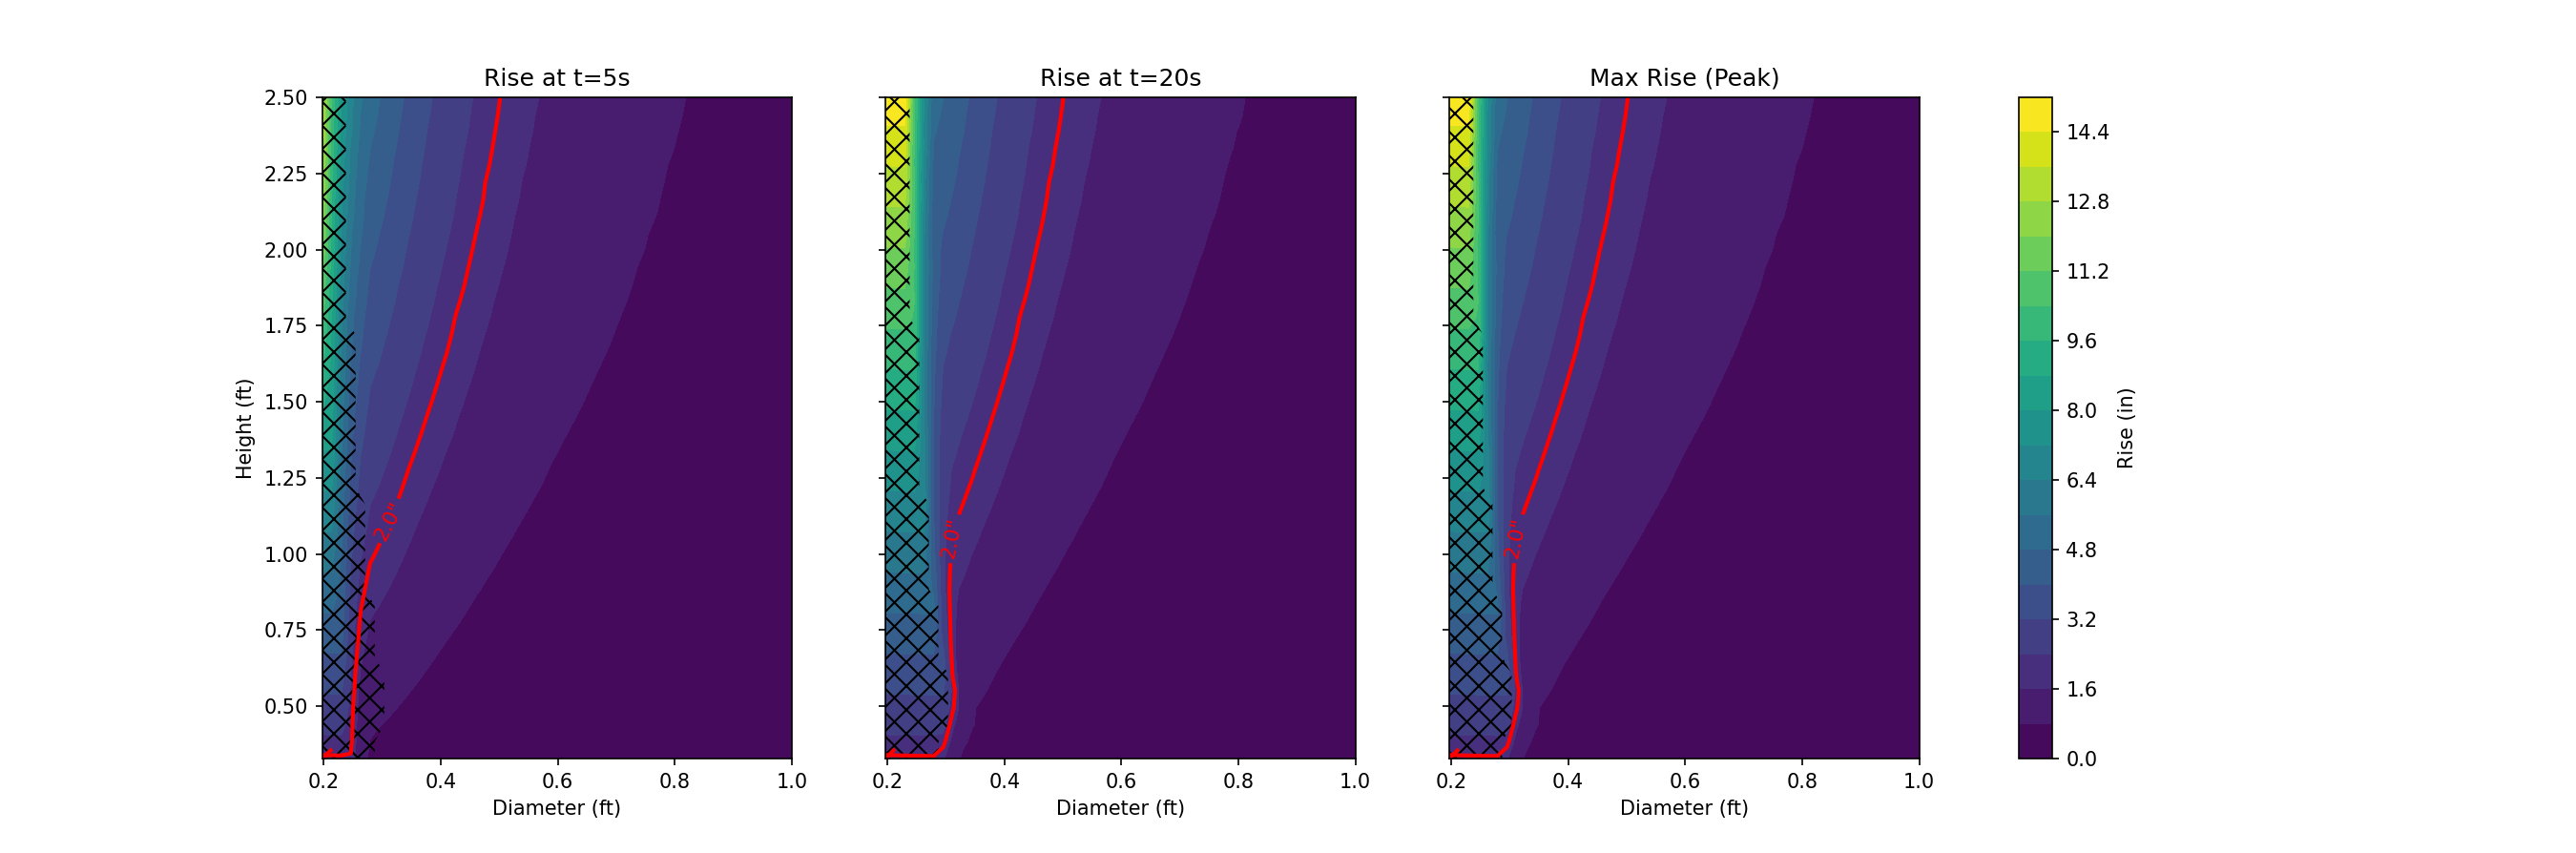
\includegraphics[width=\textwidth]{images/liqlev_50_fill_complete/plots_flow_0.004.png}
\caption{0.004\,lbm/s}
\end{subfigure}
\vspace{0.8em}    % <-- tighter vertical spacing

\begin{subfigure}[b]{0.85\textwidth}
\centering
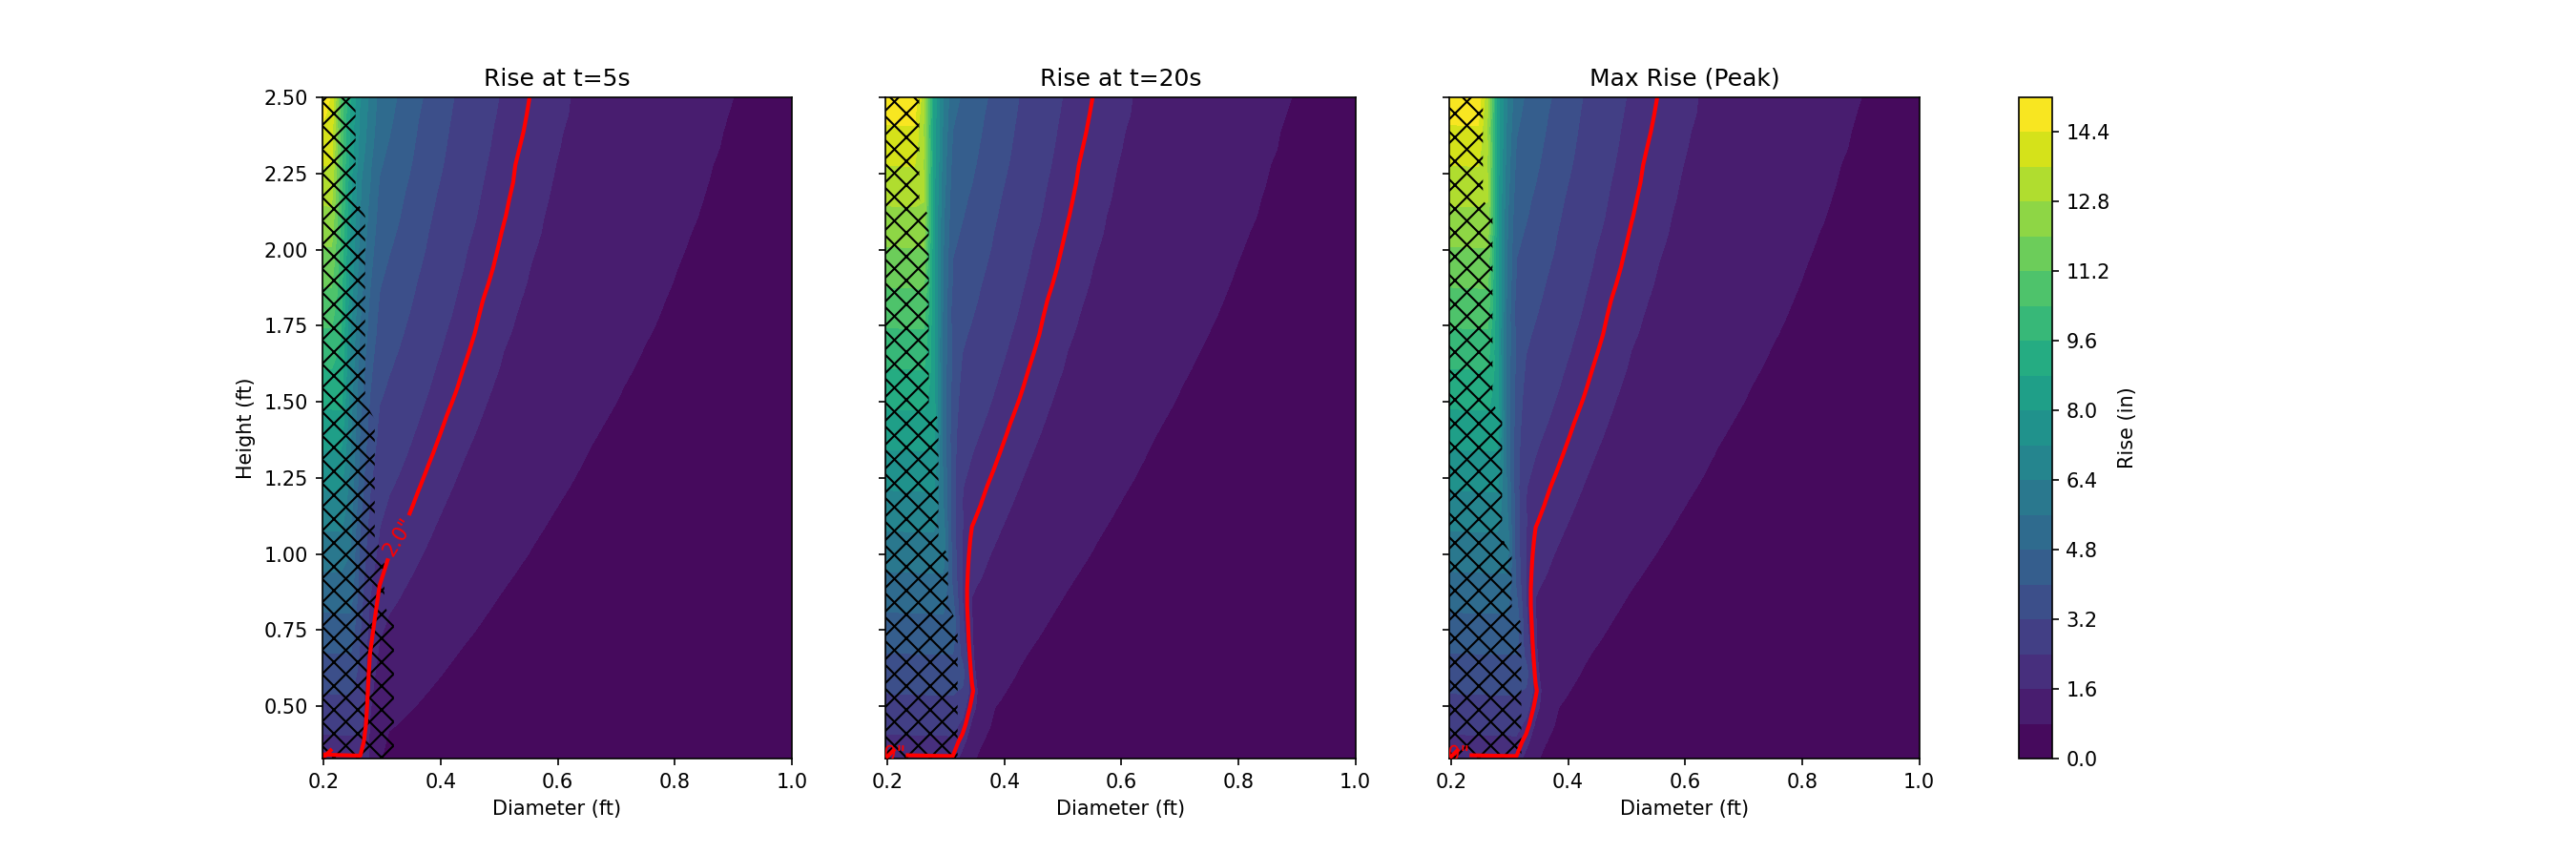
\includegraphics[width=\textwidth]{images/liqlev_50_fill_complete/plots_flow_0.005.png}
\caption{0.005\,lbm/s}
\end{subfigure}
\hspace{-0.6em}
\begin{subfigure}[b]{0.85\textwidth}
\centering
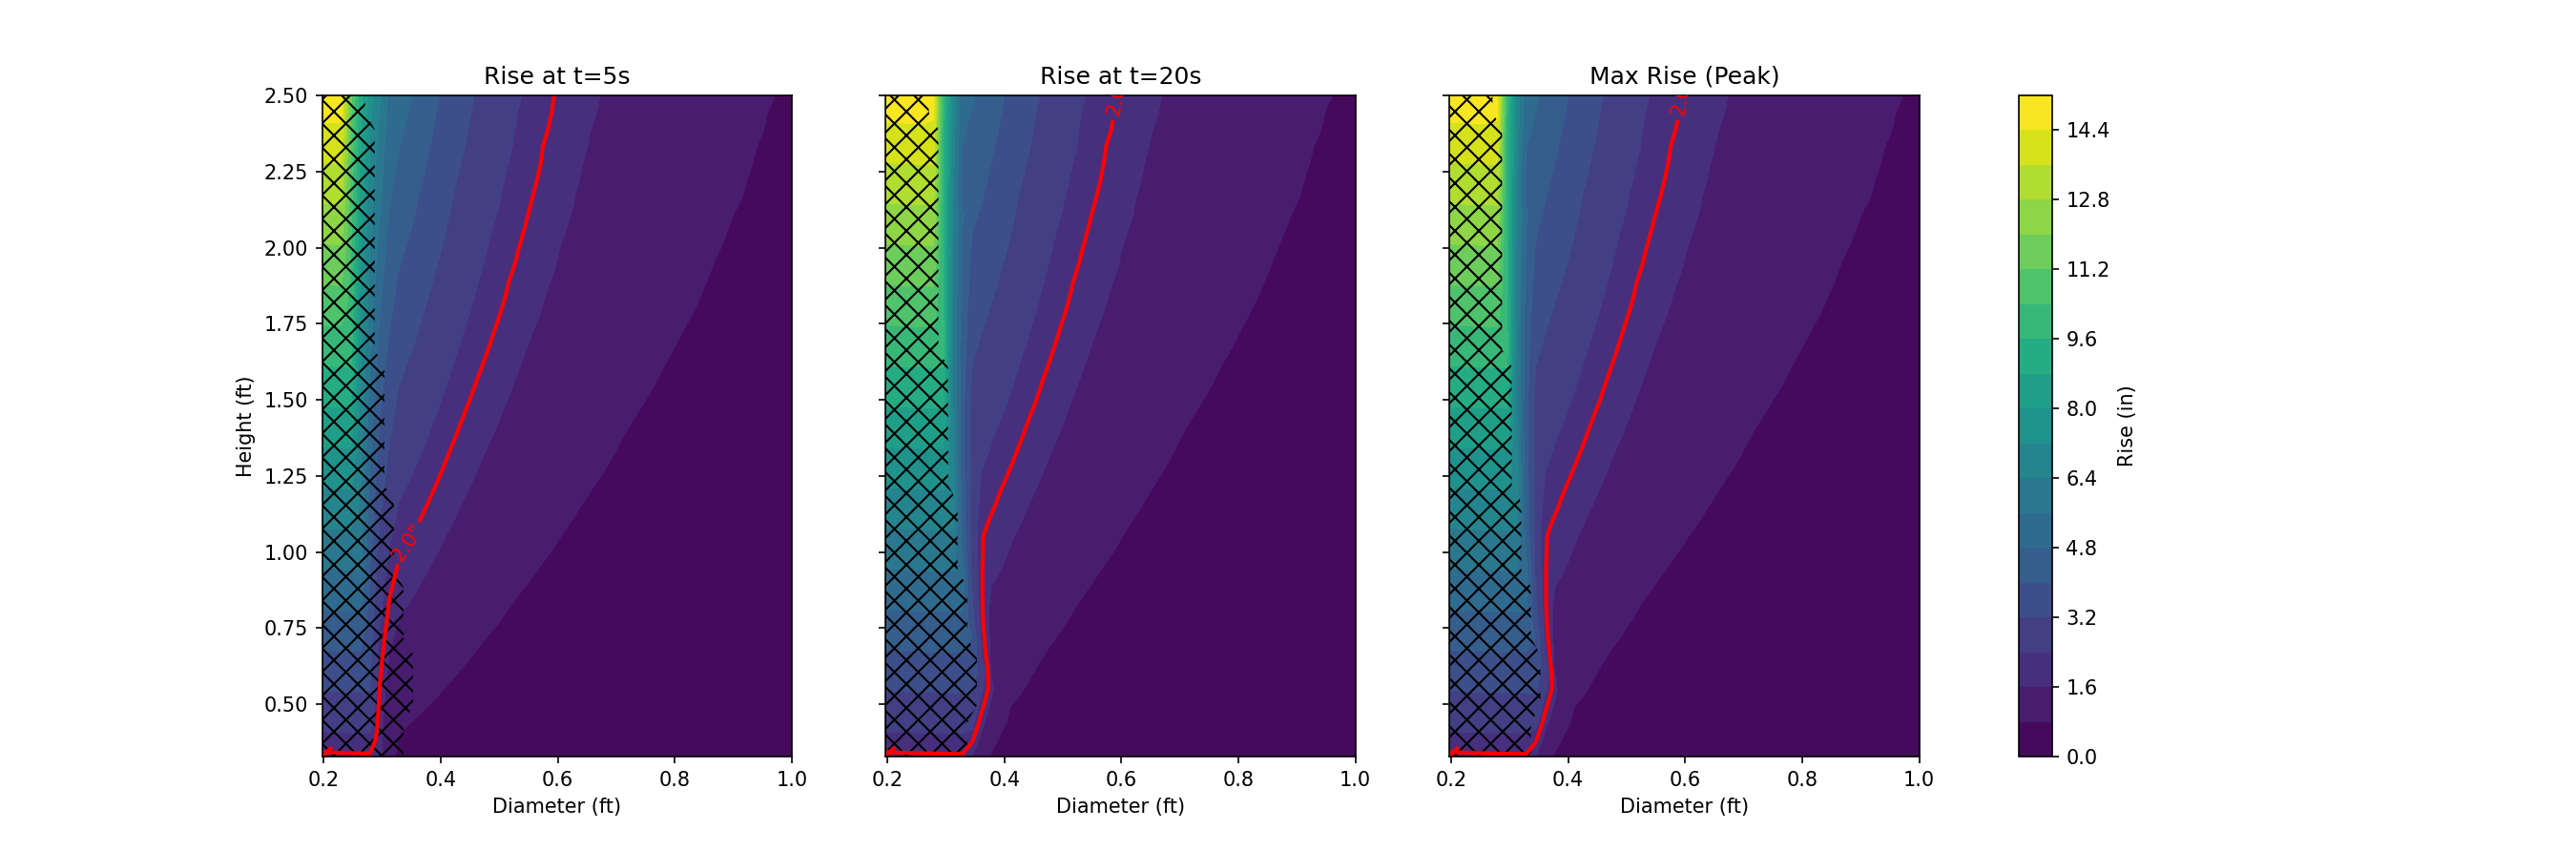
\includegraphics[width=\textwidth]{images/liqlev_50_fill_complete/plots_flow_0.006.png}
\caption{0.006\,lbm/s}
\end{subfigure}

\caption{Tank-size sweep results at 50\,\% initial fill fraction for the 5-second facility ($10^{-5}$\,g) across the four vent rates examined. Each panel shows rise (inches) at $t=5$\,s, $t=20$\,s (or end-of-run), and global peak. Red contour = 2-inch measurable threshold; hatched regions = lid impingement.}
\label{fig:sweep_50_combined}
\end{figure}

\begin{figure}[htbp]
\centering

\begin{subfigure}[b]{0.85\textwidth}
\centering
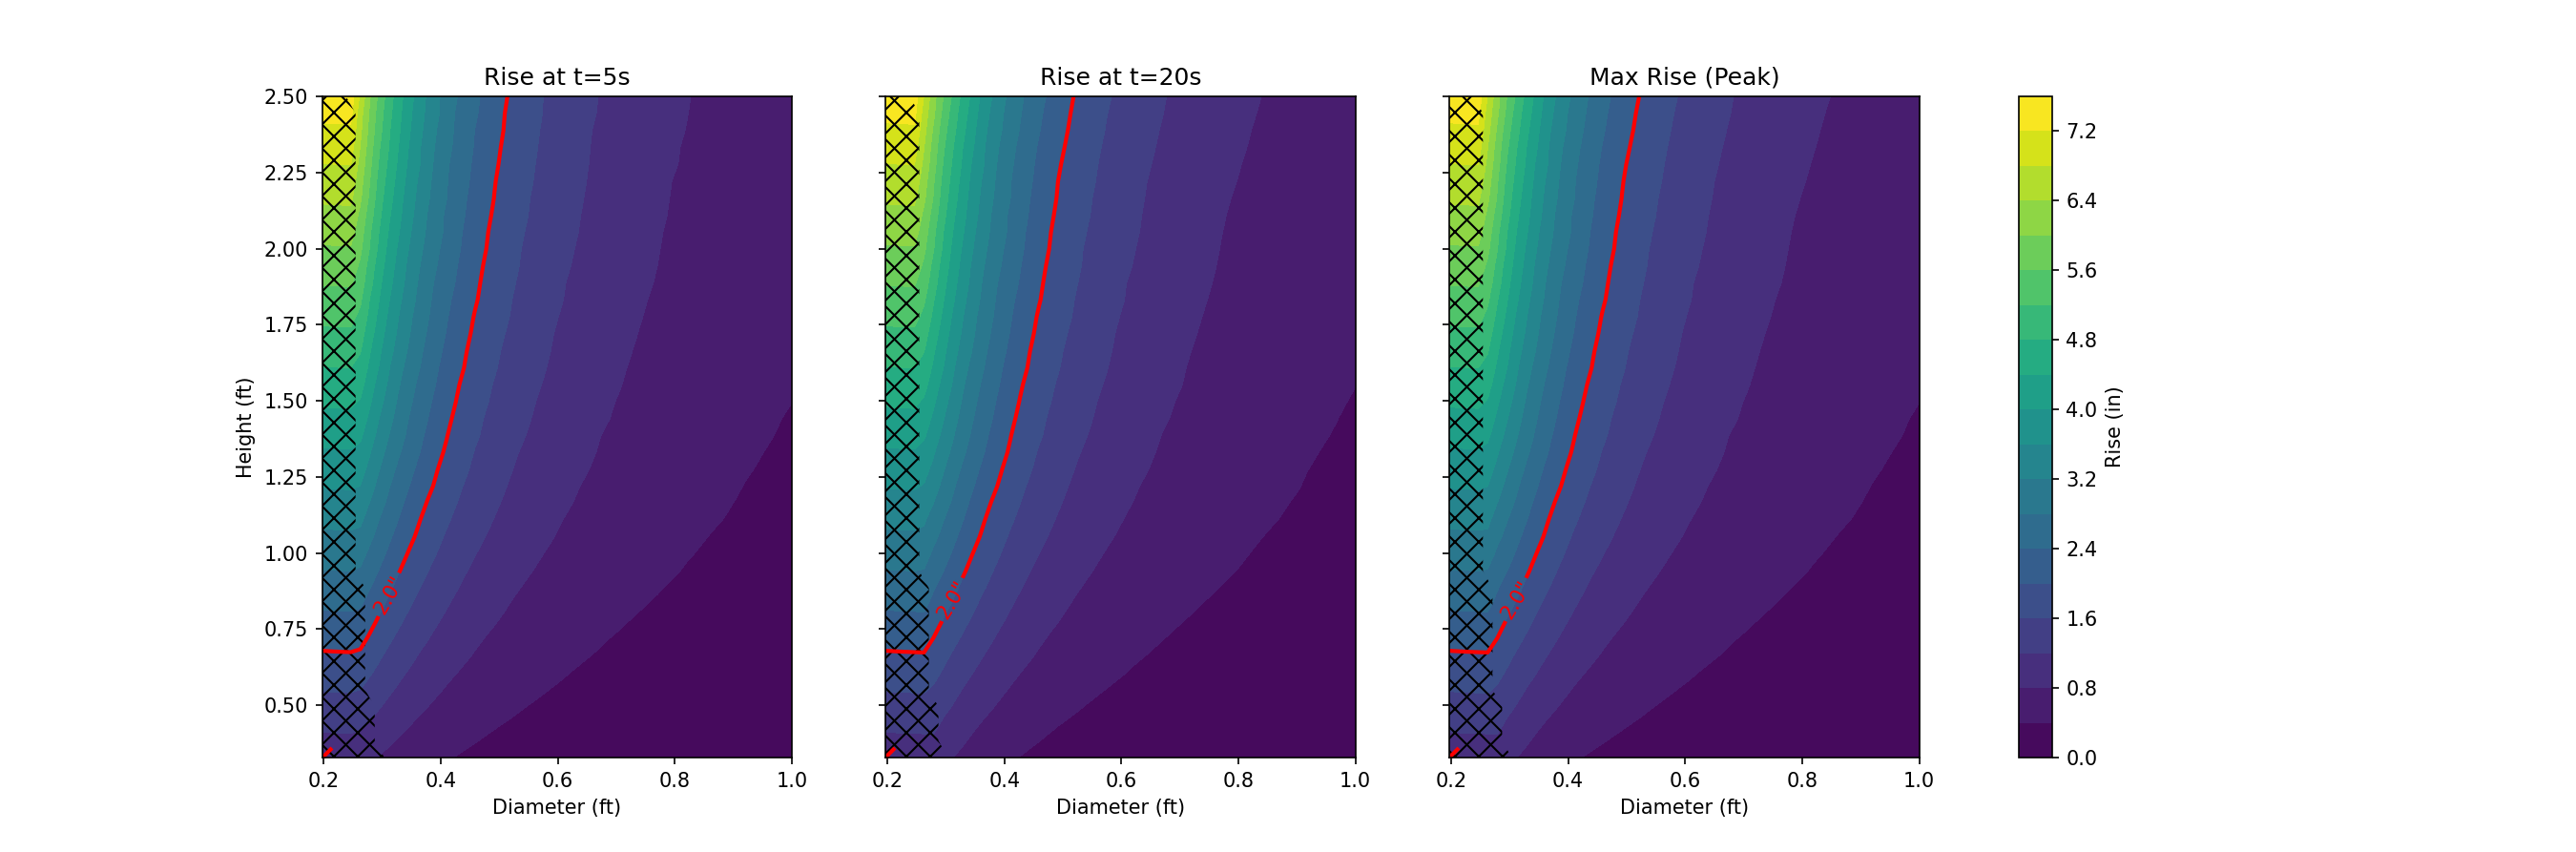
\includegraphics[width=\textwidth]{images/liqlev_75_fill_complete/plots_flow_0.003.png}
\caption{0.003\,lbm/s}
\end{subfigure}
\hspace{-0.6em}   % <-- allows gentle overlap
\begin{subfigure}[b]{0.85\textwidth}
\centering
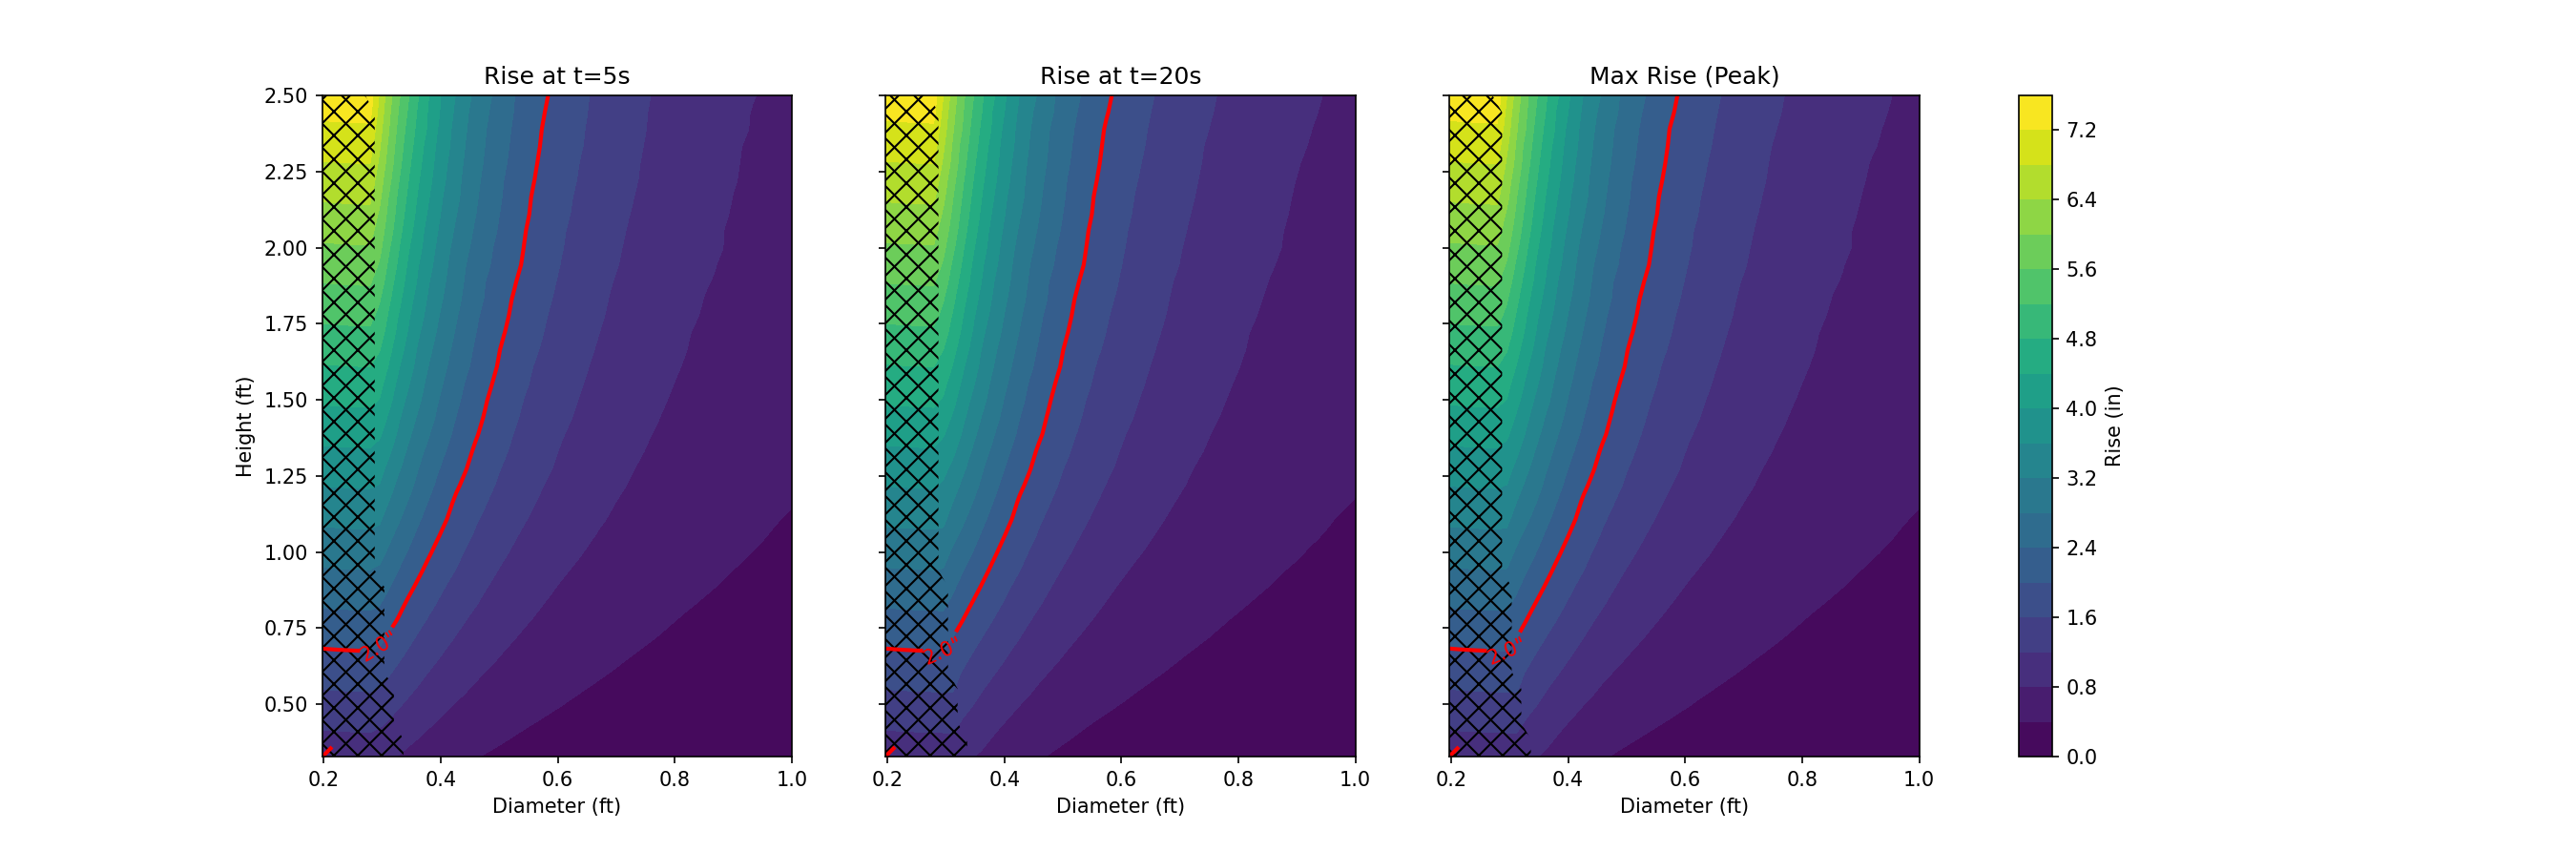
\includegraphics[width=\textwidth]{images/liqlev_75_fill_complete/plots_flow_0.004.png}
\caption{0.004\,lbm/s}
\end{subfigure}

\vspace{0.8em}    % <-- tighter vertical spacing

\begin{subfigure}[b]{0.85\textwidth}
\centering
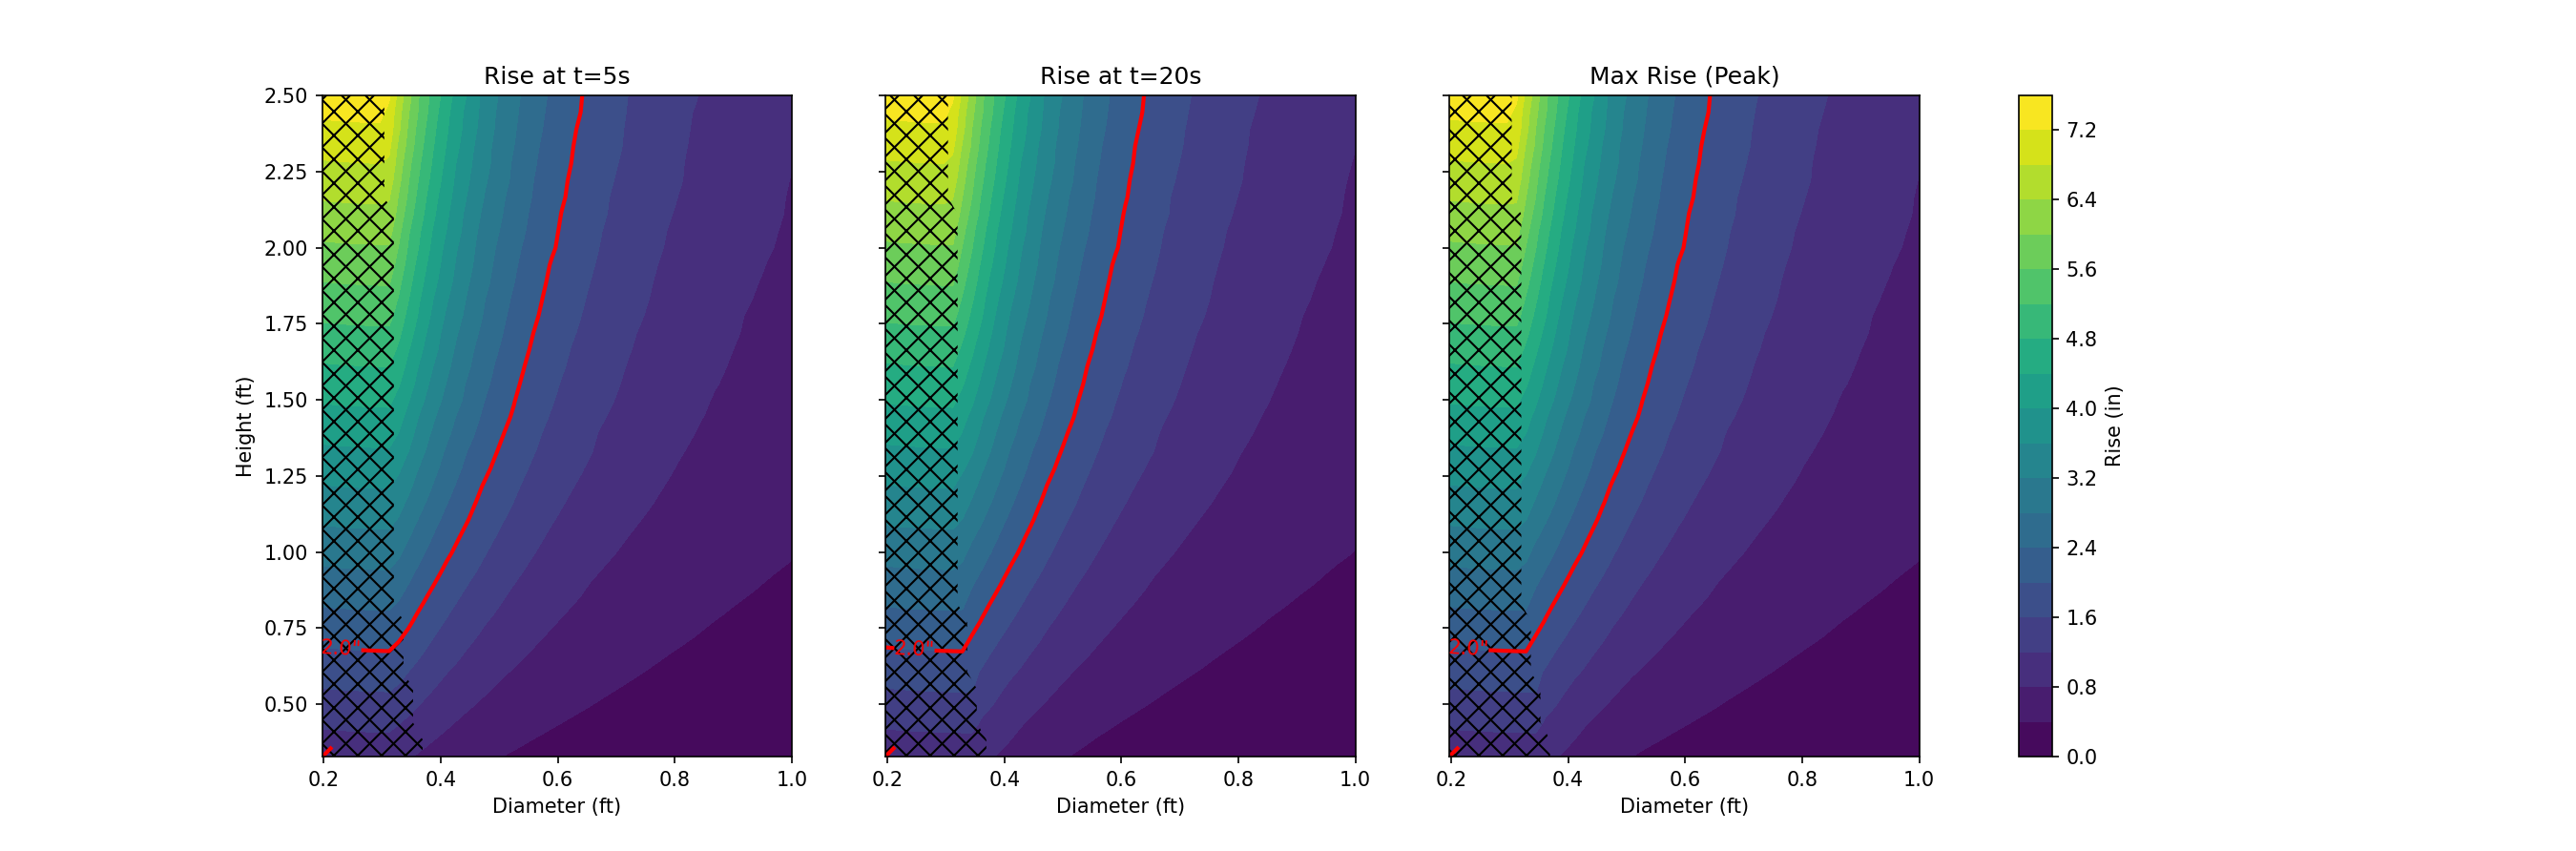
\includegraphics[width=\textwidth]{images/liqlev_75_fill_complete/plots_flow_0.005.png}
\caption{0.005\,lbm/s}
\end{subfigure}
\hspace{-0.6em}
\begin{subfigure}[b]{0.85\textwidth}
\centering
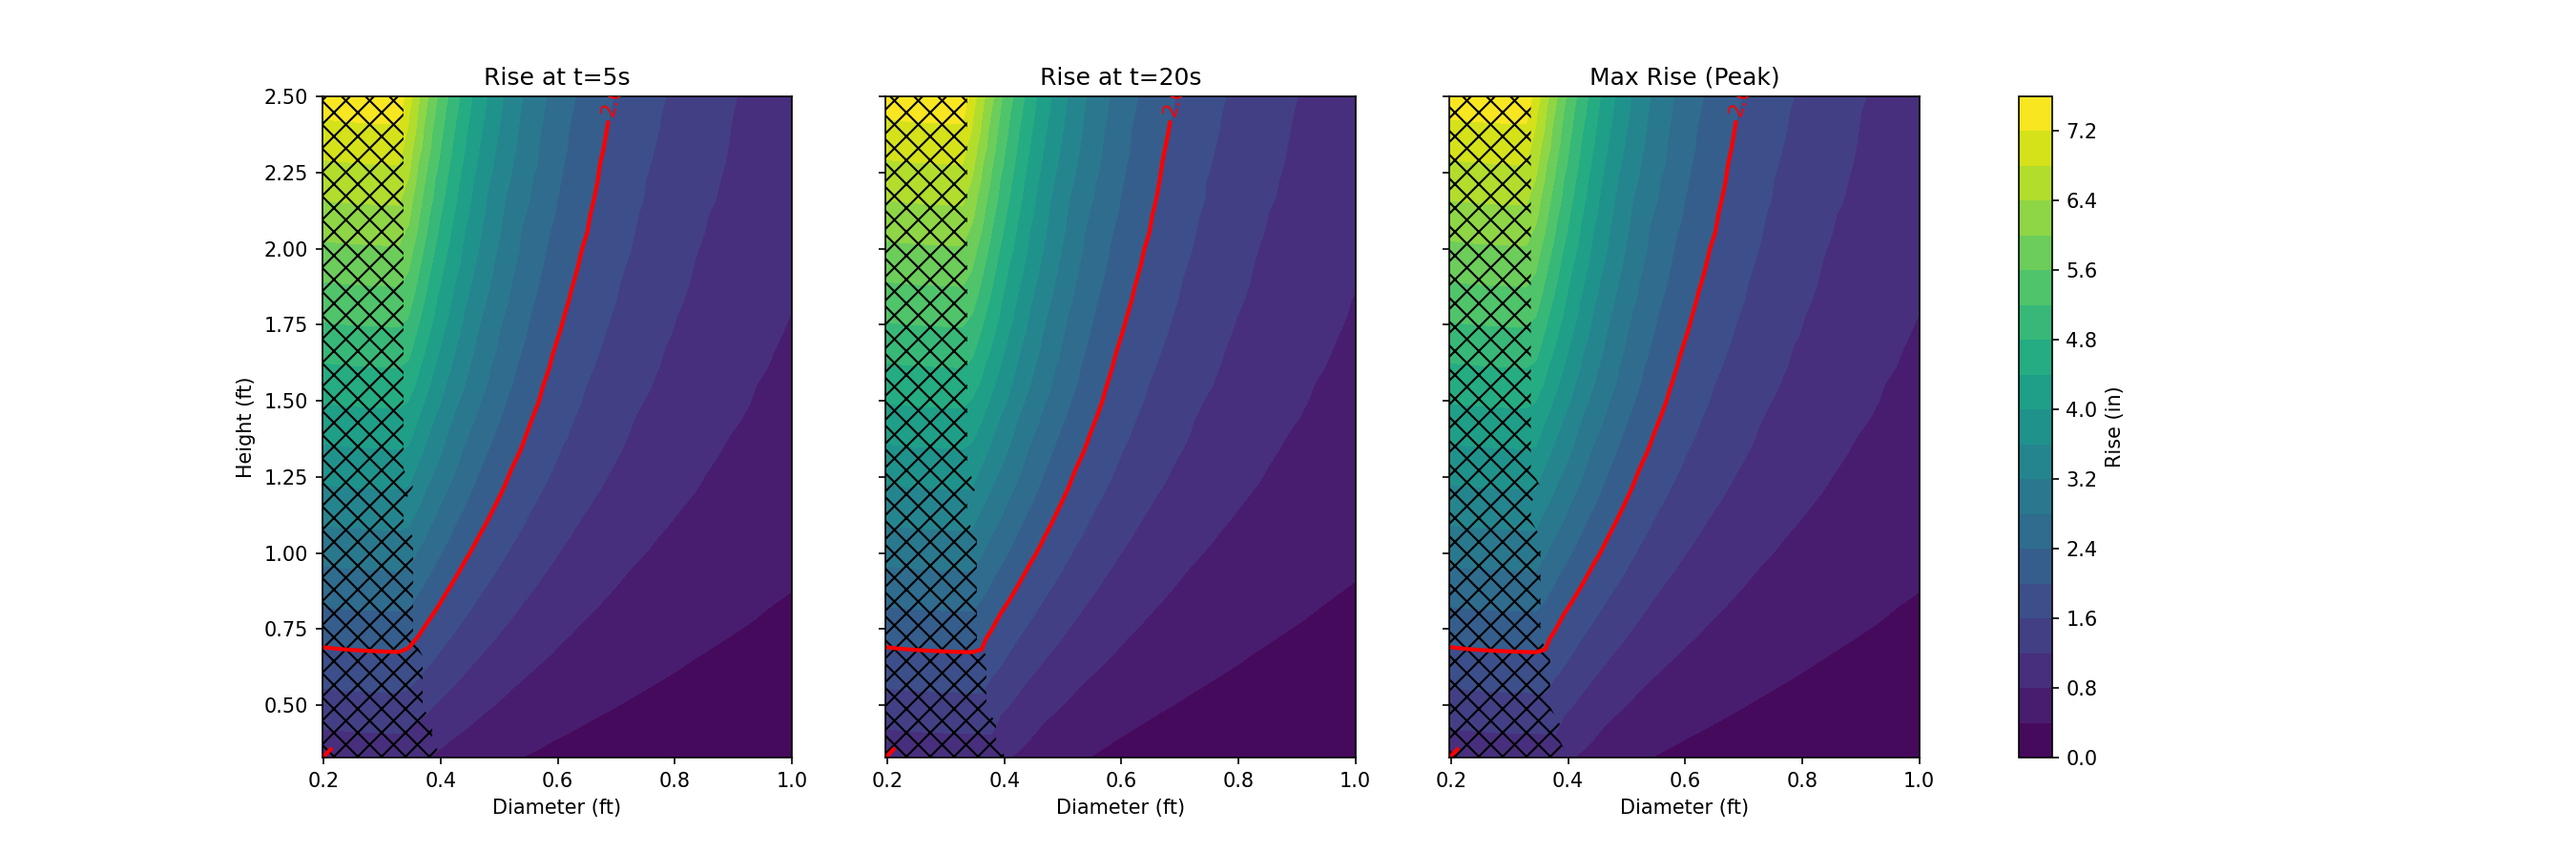
\includegraphics[width=\textwidth]{images/liqlev_75_fill_complete/plots_flow_0.006.png}
\caption{0.006\,lbm/s}
\end{subfigure}

\caption{Tank-size sweep results at 75\,\% initial fill fraction for the 5-second facility ($10^{-5}$\,g) across the four vent rates examined. Each panel shows rise (inches) at $t=5$\,s, $t=20$\,s (or end-of-run), and global peak. Red contour = 2-inch measurable threshold; hatched regions = lid impingement.}
\label{fig:sweep_75_combined}
\end{figure}


\subsection{Facility-Specific Performance and Optimal Test Matrix}

\textbf{Parabolic Flight:}
The facility provides approximately 17\,s of reduced gravity, nominally $\sim10^{-2}$\,g with typical g-jitter. Simulations for this platform were performed using the geometry of an existing parabolic-flight test tank designed for microgravity pool boiling experiments in liquid nitrogen \cite{Opitz2021}. The tank is a vacuum-jacketed, double-walled stainless-steel 304L cylindrical dewar with a 100-liter LN$_2$ capacity and a maximum pressure rating of 90\,psig. Although the extended duration would have permitted the wall thermal boundary layer to fully develop after initial meniscus reorientation, allowing the liquid-vapor interface to approach a quasi-steady boiling state, parabolic flight was ultimately not pursued. High-fidelity analysis identified persistent lateral acceleration components (typically $10^{-2}$ to $5\times10^{-3}$\,g) inherent to the parabolic maneuver and aircraft attitude corrections. These lateral vectors excite unidirectional sloshing and asymmetric interfacial modes that contaminate the purely thermodynamic, boundary-layer-driven liquid level rise of primary interest.

This conclusion was supported by transient CFD simulations incorporating full three-axis acceleration time histories from representative parabolic-flight profiles, as well as independent experimental observations from published parabolic sloshing studies. Consequently, the platform-specific vent rates required to achieve measurable rises (2+ inches) and the associated maximum fill fractions to avoid lid impingement were not advanced.

Variable-gravity profiles were nevertheless evaluated in the LIQLEV model using conservative acceleration magnitudes ($\sqrt{g_x^2 + g_y^2 + g_z^2}$). These simulations indicated that rises of at least 3 inches could be achieved during the low-g plateau; however, the risk of lateral sloshing precluded further consideration of parabolic flight as a test venue.


\textbf{GRC 2.2-Second Drop Tower:} 
The facility operates over a gravity range of $\sim10^{-3}$ to $10^{-5}$\,g. Comprehensive parametric investigations covering a broad matrix of tank diameters, aspect ratios, initial fill fractions, and vent flow rates demonstrated that the severely constrained 2.2-second test window is generally too short for the liquid-vapor interface to reach its maximum thermodynamic level rise. Even when employing high initial fill fractions ($\sim$75--80\,\%) and aggressive initial vent rates (0.25--0.75\,lbm/s) to drive rapid interface motion within the first 1.5--2\,s, the model shows that only the early transient phase of boundary-layer vapor generation and liquid displacement can be captured, without sufficient time for sustained boiling to develop the peak rise. 

In comparison, the NASA GRC 5-second zero-gravity facility provides both a longer test duration and a lower residual gravity level ($\sim10^{-5}$\,g), enabling substantially higher measurable peak liquid level rise once the experimental configuration has been carefully optimized. Consequently, achieving a measurable peak rise in the 2.2-second facility would require even skinnier tanks and substantially higher vent rates (at the same fill level) than those viable in the 5-second facility. Such geometries, however, would no longer fit within the physical envelope of existing drop capsules.

\textbf{GRC 5-Second Zero-Gravity Facility:} 
The facility operates at $\sim10^{-5}$\,g. Comprehensive parametric sweeps encompassing thousands of tank geometries (diameters 0.2--1.0\,ft, heights 0.3--2.5\,ft), initial fill fractions, vent flow rates, and $\epsilon$ schedules identified this platform as the optimal test venue. It provides the ideal balance of true high-quality microgravity and sufficient test duration for the wall boundary-layer vapor generation and resulting liquid displacement to develop fully, enabling the liquid-vapor interface to attain its maximum thermodynamic rise—unlike the severely time-constrained 2.2-second facility. The low residual gravity further enhances measurable interface displacement by minimizing buoyant bubble departure and increasing vapor residence time within the bulk liquid column, producing substantially larger rises than those achievable under the higher-g environments typical of parabolic flight. 

Recommended configurations utilize a small-diameter cylindrical tank (0.3\,ft diameter $\times$ 2.0\,ft height, $L/D \approx 6.67$) with initial fill fractions of 40--65\% and moderate constant vent rates (0.003--0.006\,lbm/s for Nitrogen). Under these optimized conditions, the peak rise is typically attained between 3.5 and 4.8\,s, comfortably within the available window and without lid impingement, thereby delivering clean, high-value optical data on sustained thermodynamic venting suitable for CFD correlation development.

These trends are illustrated in the transient response plots for the recommended 0.3\,ft $\times$ 2.0\,ft tank at 25\,\%, 50\,\%, and 75\,\% initial fill fractions (Figure~\ref{fig:0p3ft_time_histories}). The left column shows ullage pressure decay, while the right column shows liquid level rise (inches) versus time for each of the four vent rates. Green stars mark the global peak rise; red crosses indicate cases where the interface exceeded the tank height. The plots confirm that 40--65\,\% fill fractions with the selected vent rates produce measurable rises of 2--8 inches that peak well before the end of the 5-second window, while 75\,\% fill leads to early impingement at the higher vent rates, reinforcing the recommended upper fill limit.

% \begin{figure}[htbp]
% \centering
% 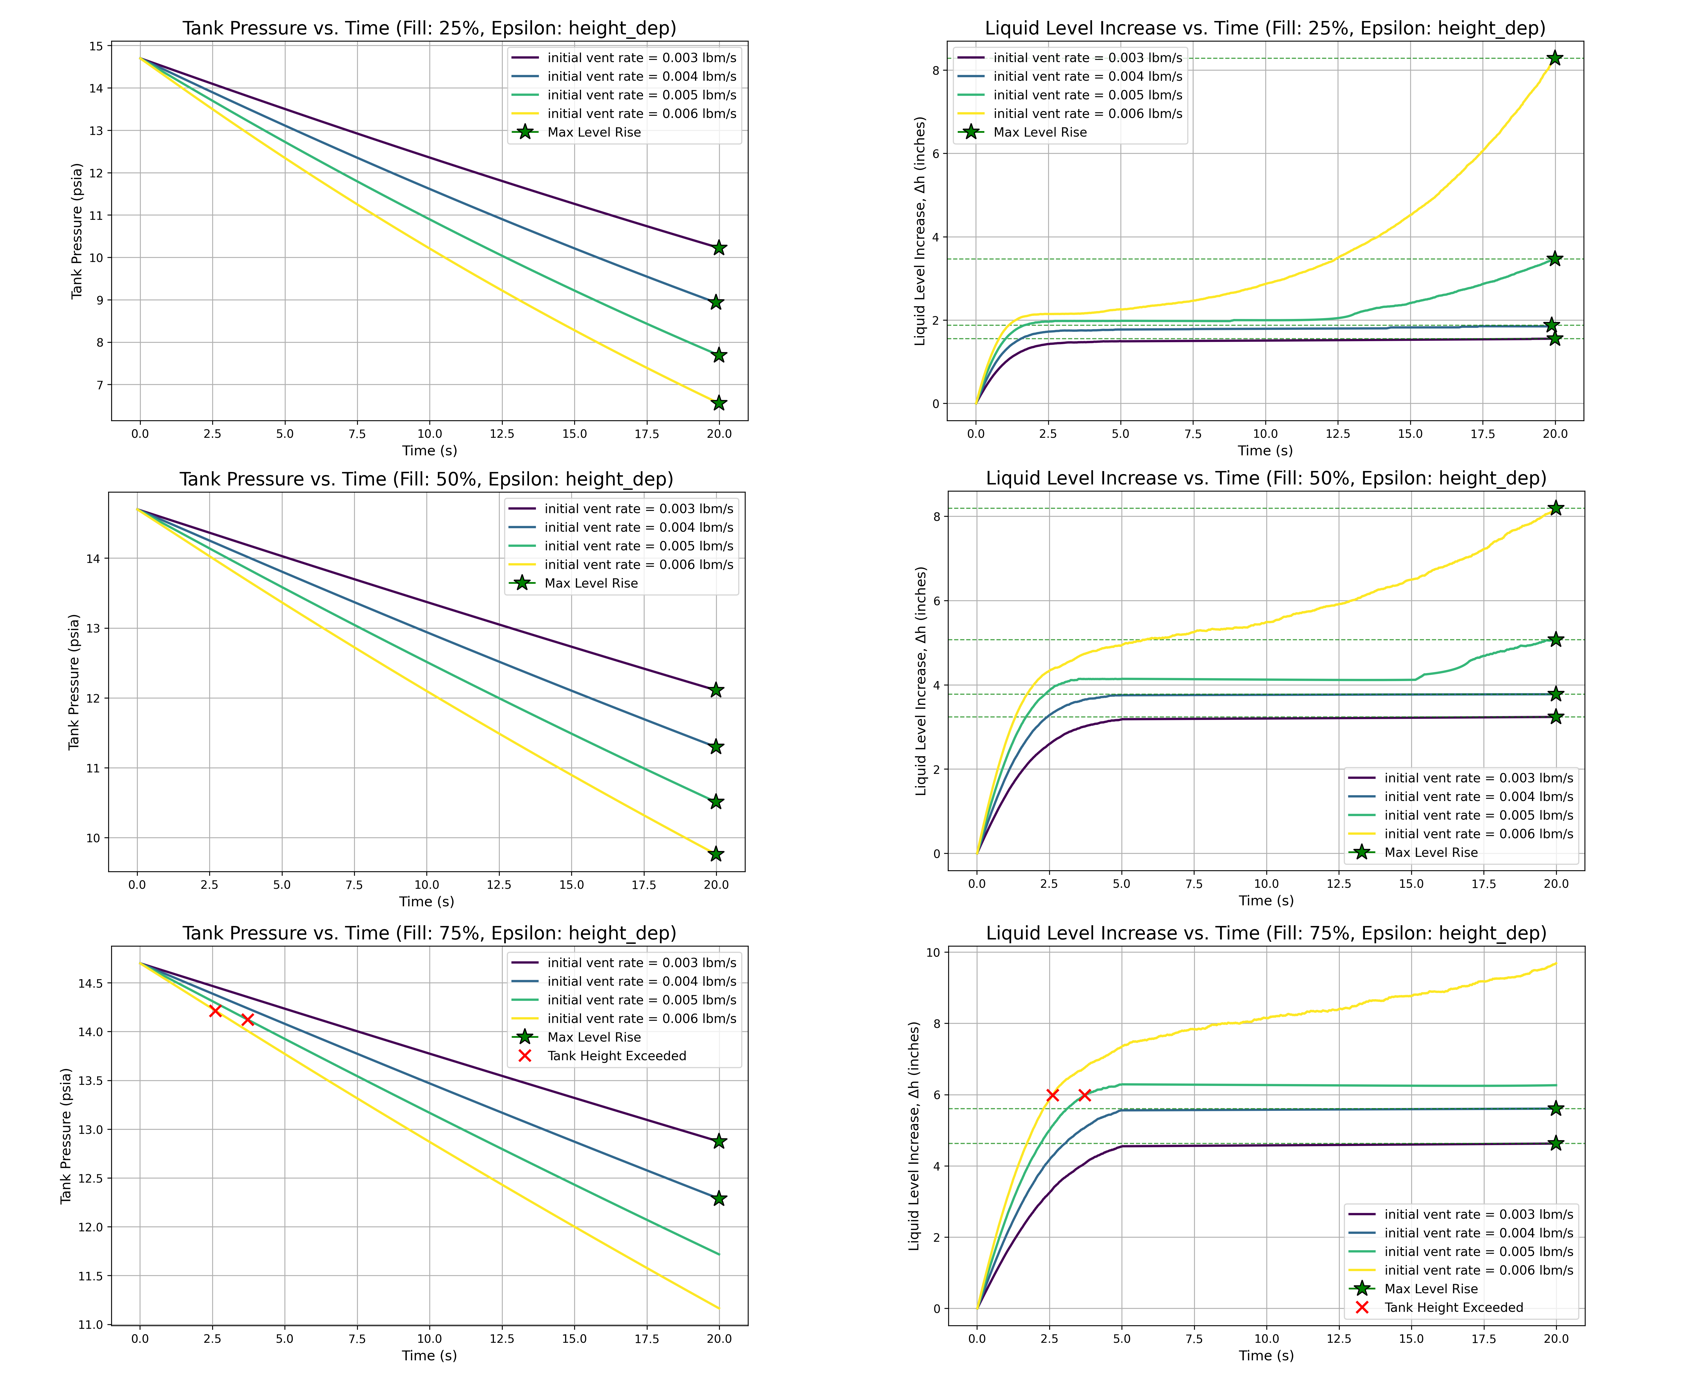
\includegraphics[width=\textwidth]{images/0p3ft_x_2ft_level_rise.png}
% \caption{Transient response of the recommended 0.3\,ft diameter $\times$ 2.0\,ft height tank in the 5-second facility using the height-dependent $\epsilon$ formulation. Left column: tank pressure versus time. Right column: liquid level rise (inches) versus time. Green stars denote the global maximum rise; red crosses indicate cases where the interface exceeded the tank height.}
% \label{fig:0p3ft_time_histories}
% \end{figure}

\begin{figure}[htbp]
    \centering
    
    % --- Row 1: 25% Fill ---
    \begin{subfigure}[b]{0.48\textwidth}
        \centering
        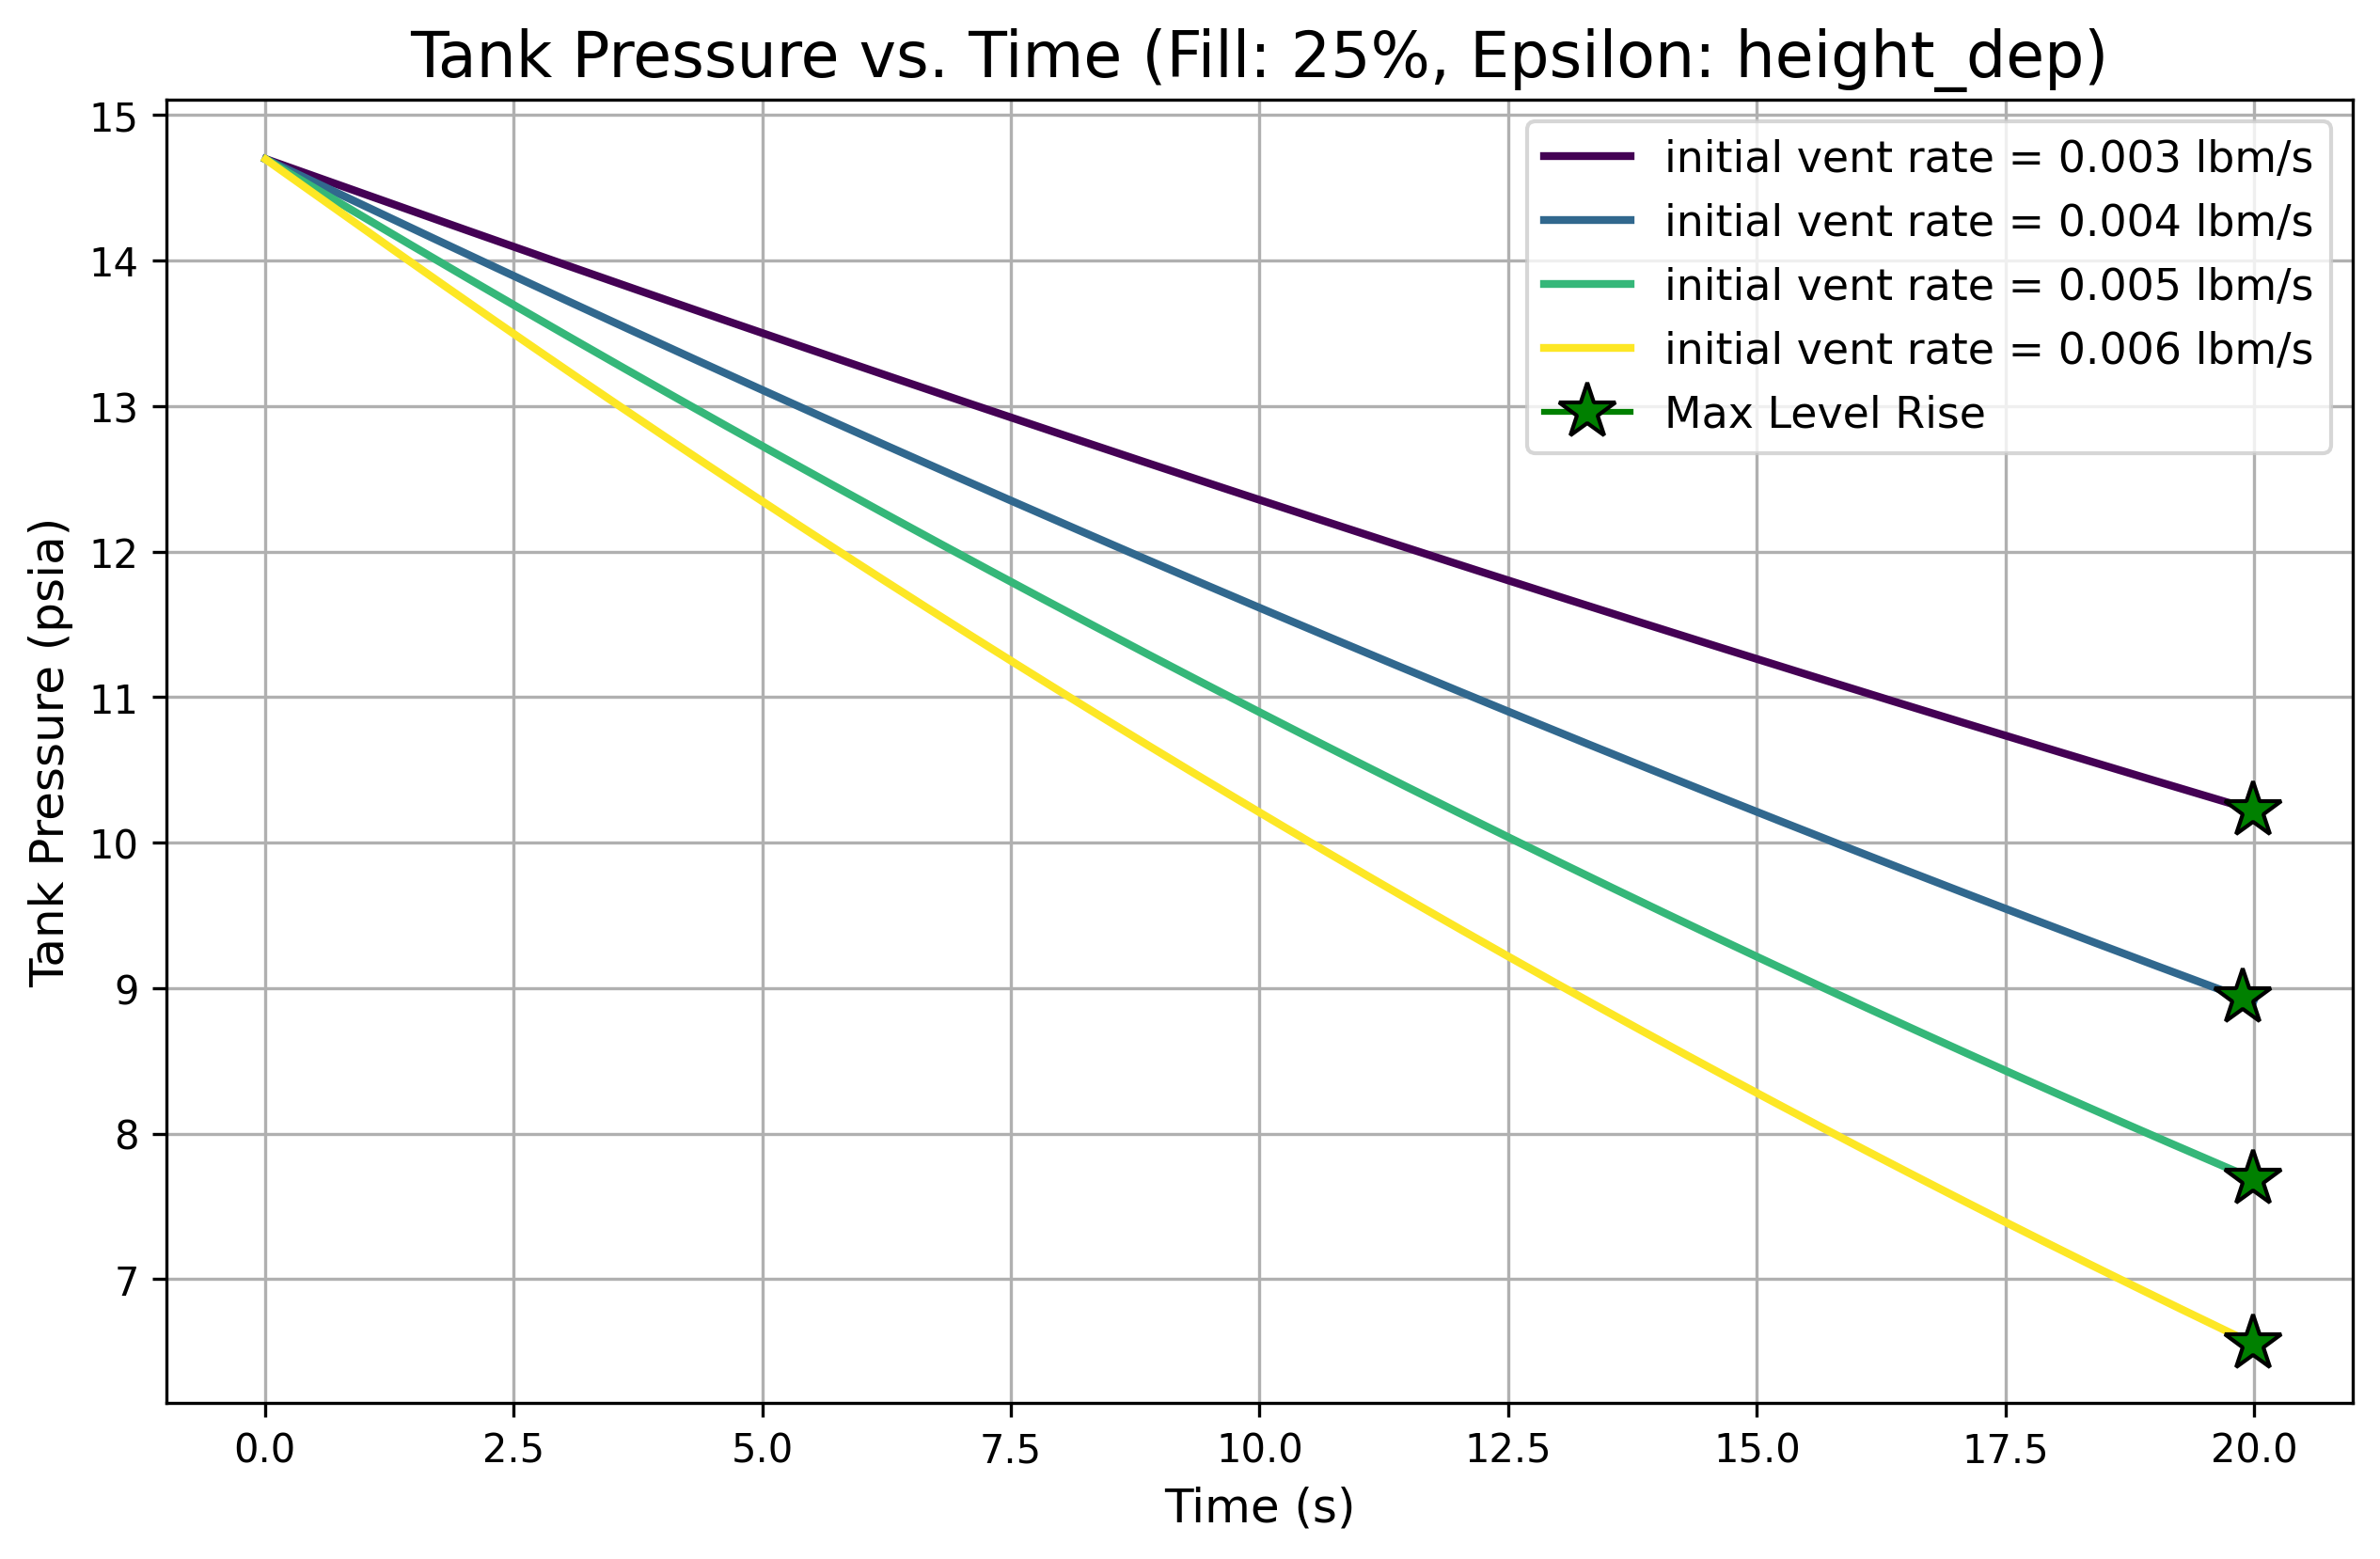
\includegraphics[width=\textwidth]{images/liqlev_0p3ftx2ft_all_vent/25_fill_pressure_height_dep.png}
        \caption{25\% Fill: Pressure}
        \label{fig:25_pressure}
    \end{subfigure}
    \hfill
    \begin{subfigure}[b]{0.48\textwidth}
        \centering
        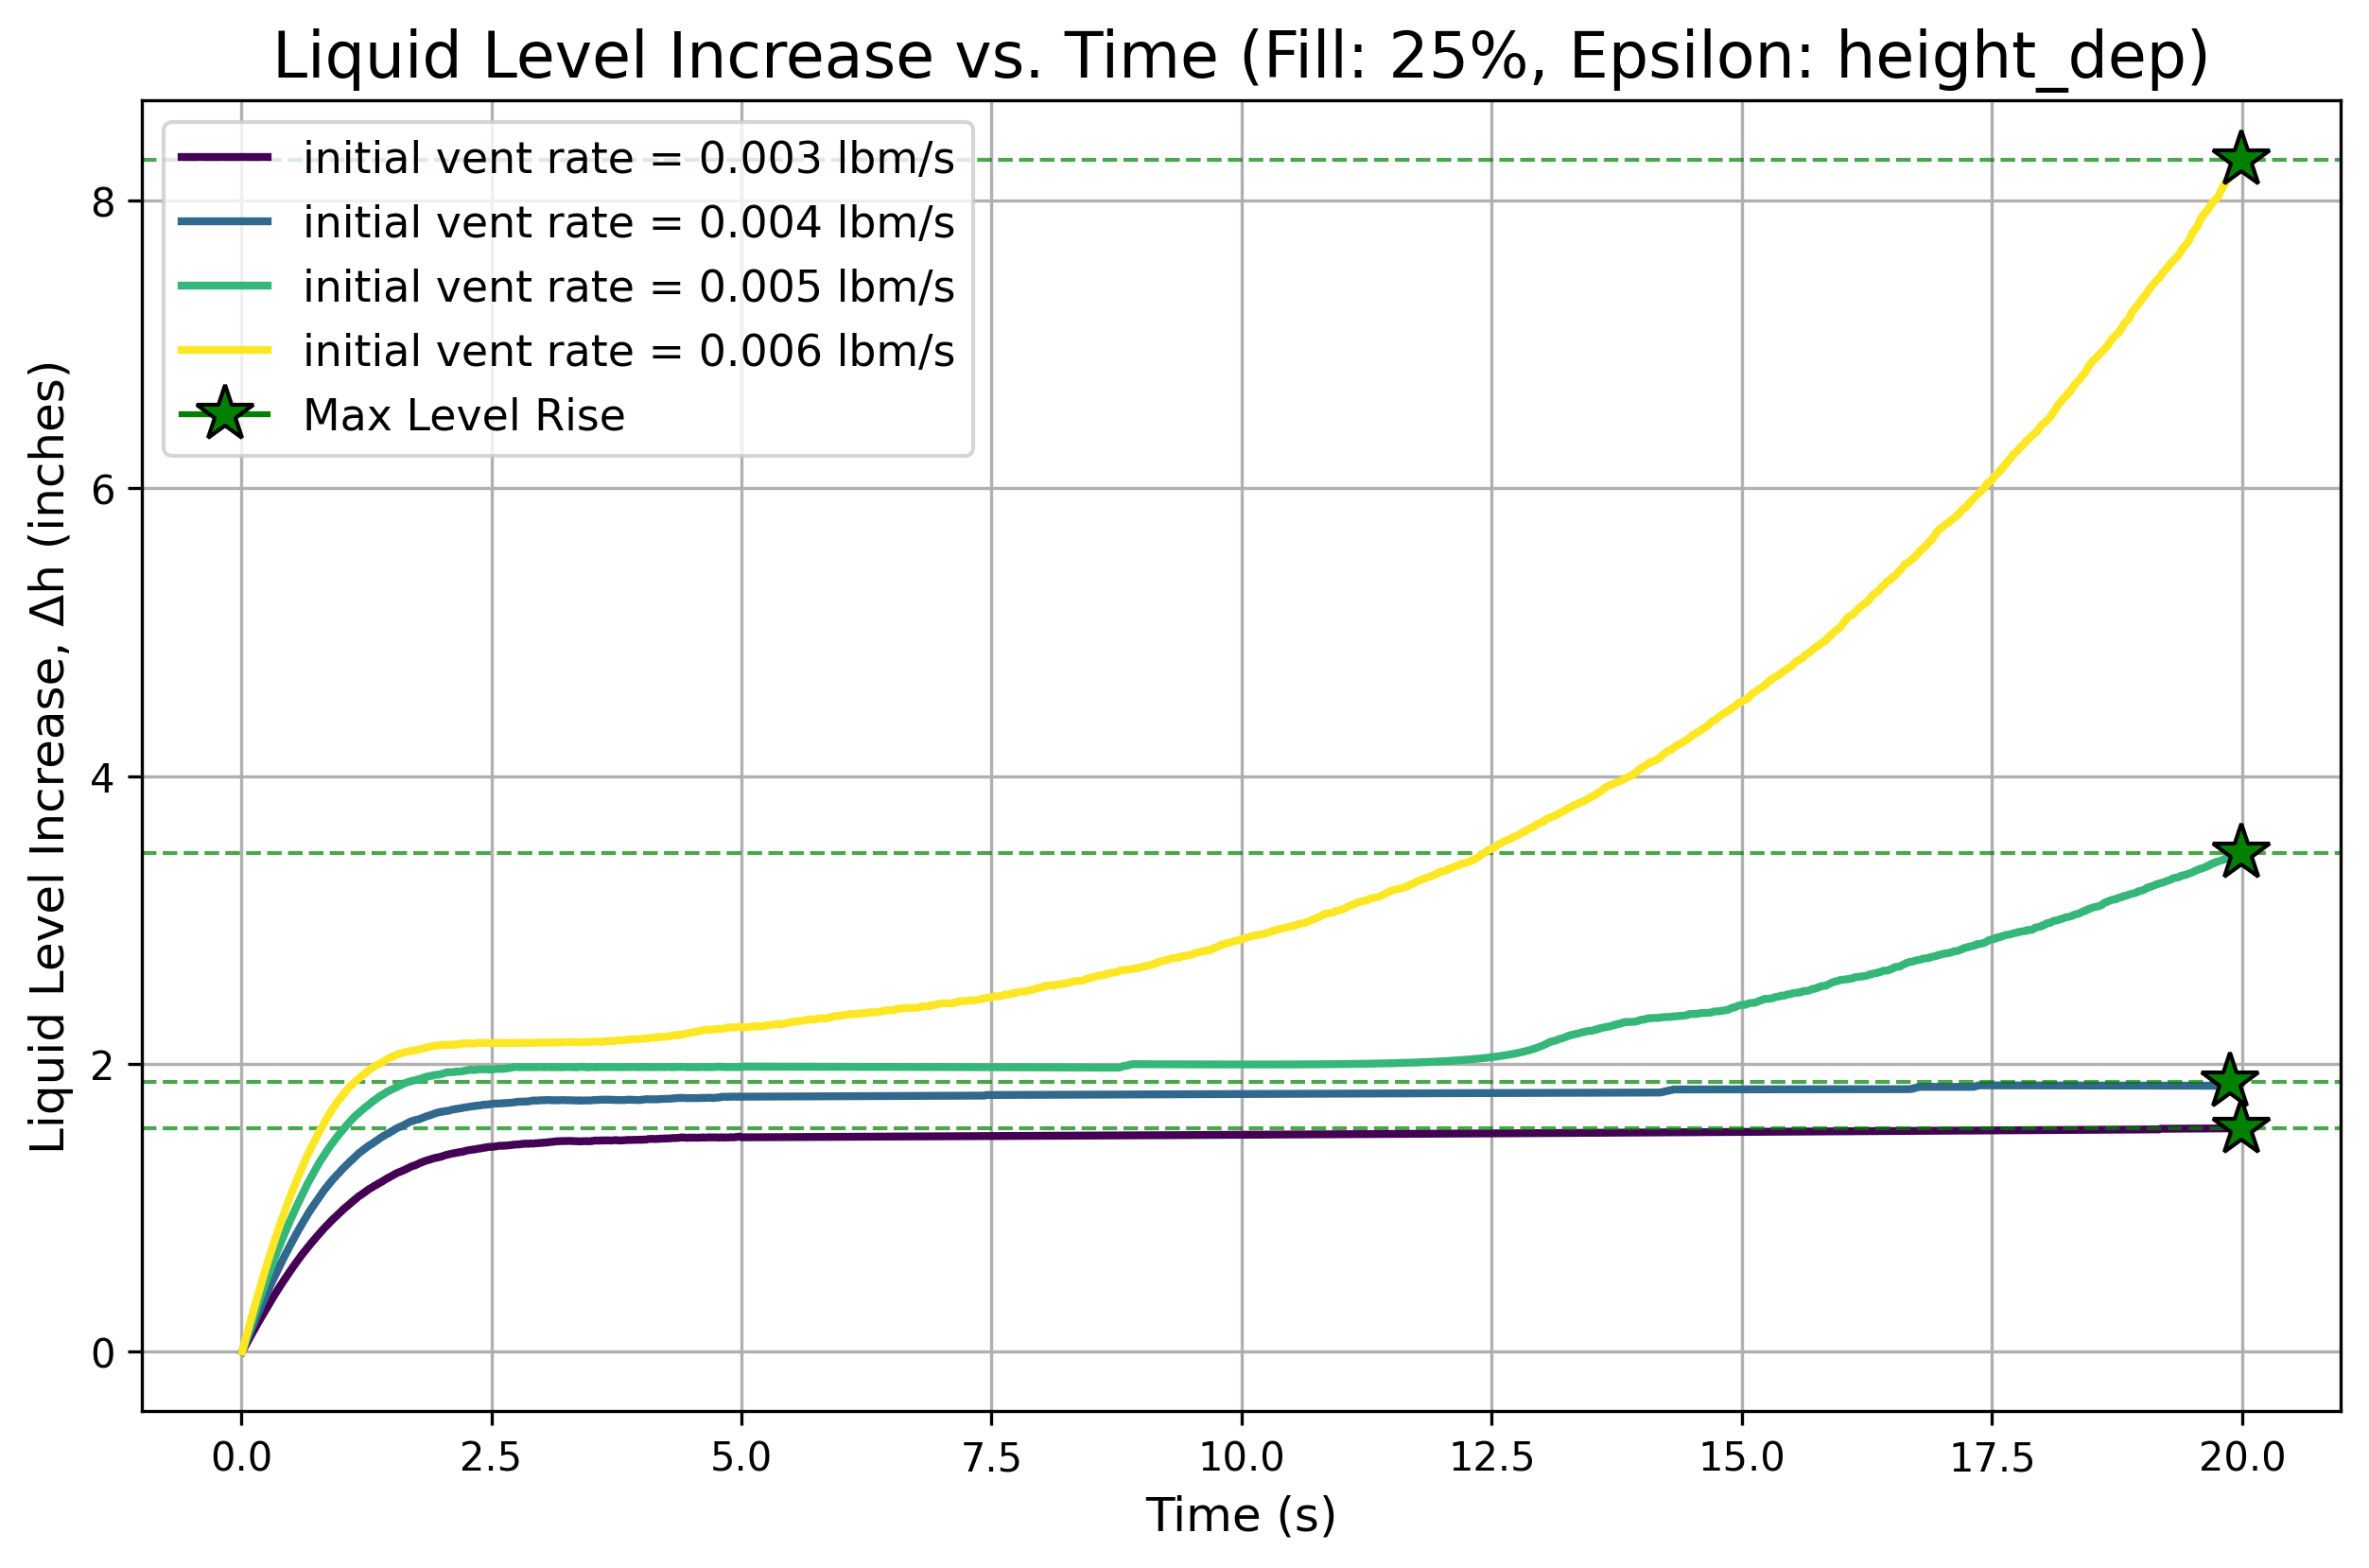
\includegraphics[width=\textwidth]{images/liqlev_0p3ftx2ft_all_vent/25_fill_liqlev_height_dep.png}
        \caption{25\% Fill: Liquid Level}
        \label{fig:25_level}
    \end{subfigure}
    
    \vspace{0.4cm} % Vertical space between rows
    
    % --- Row 2: 50% Fill ---
    \begin{subfigure}[b]{0.48\textwidth}
        \centering
        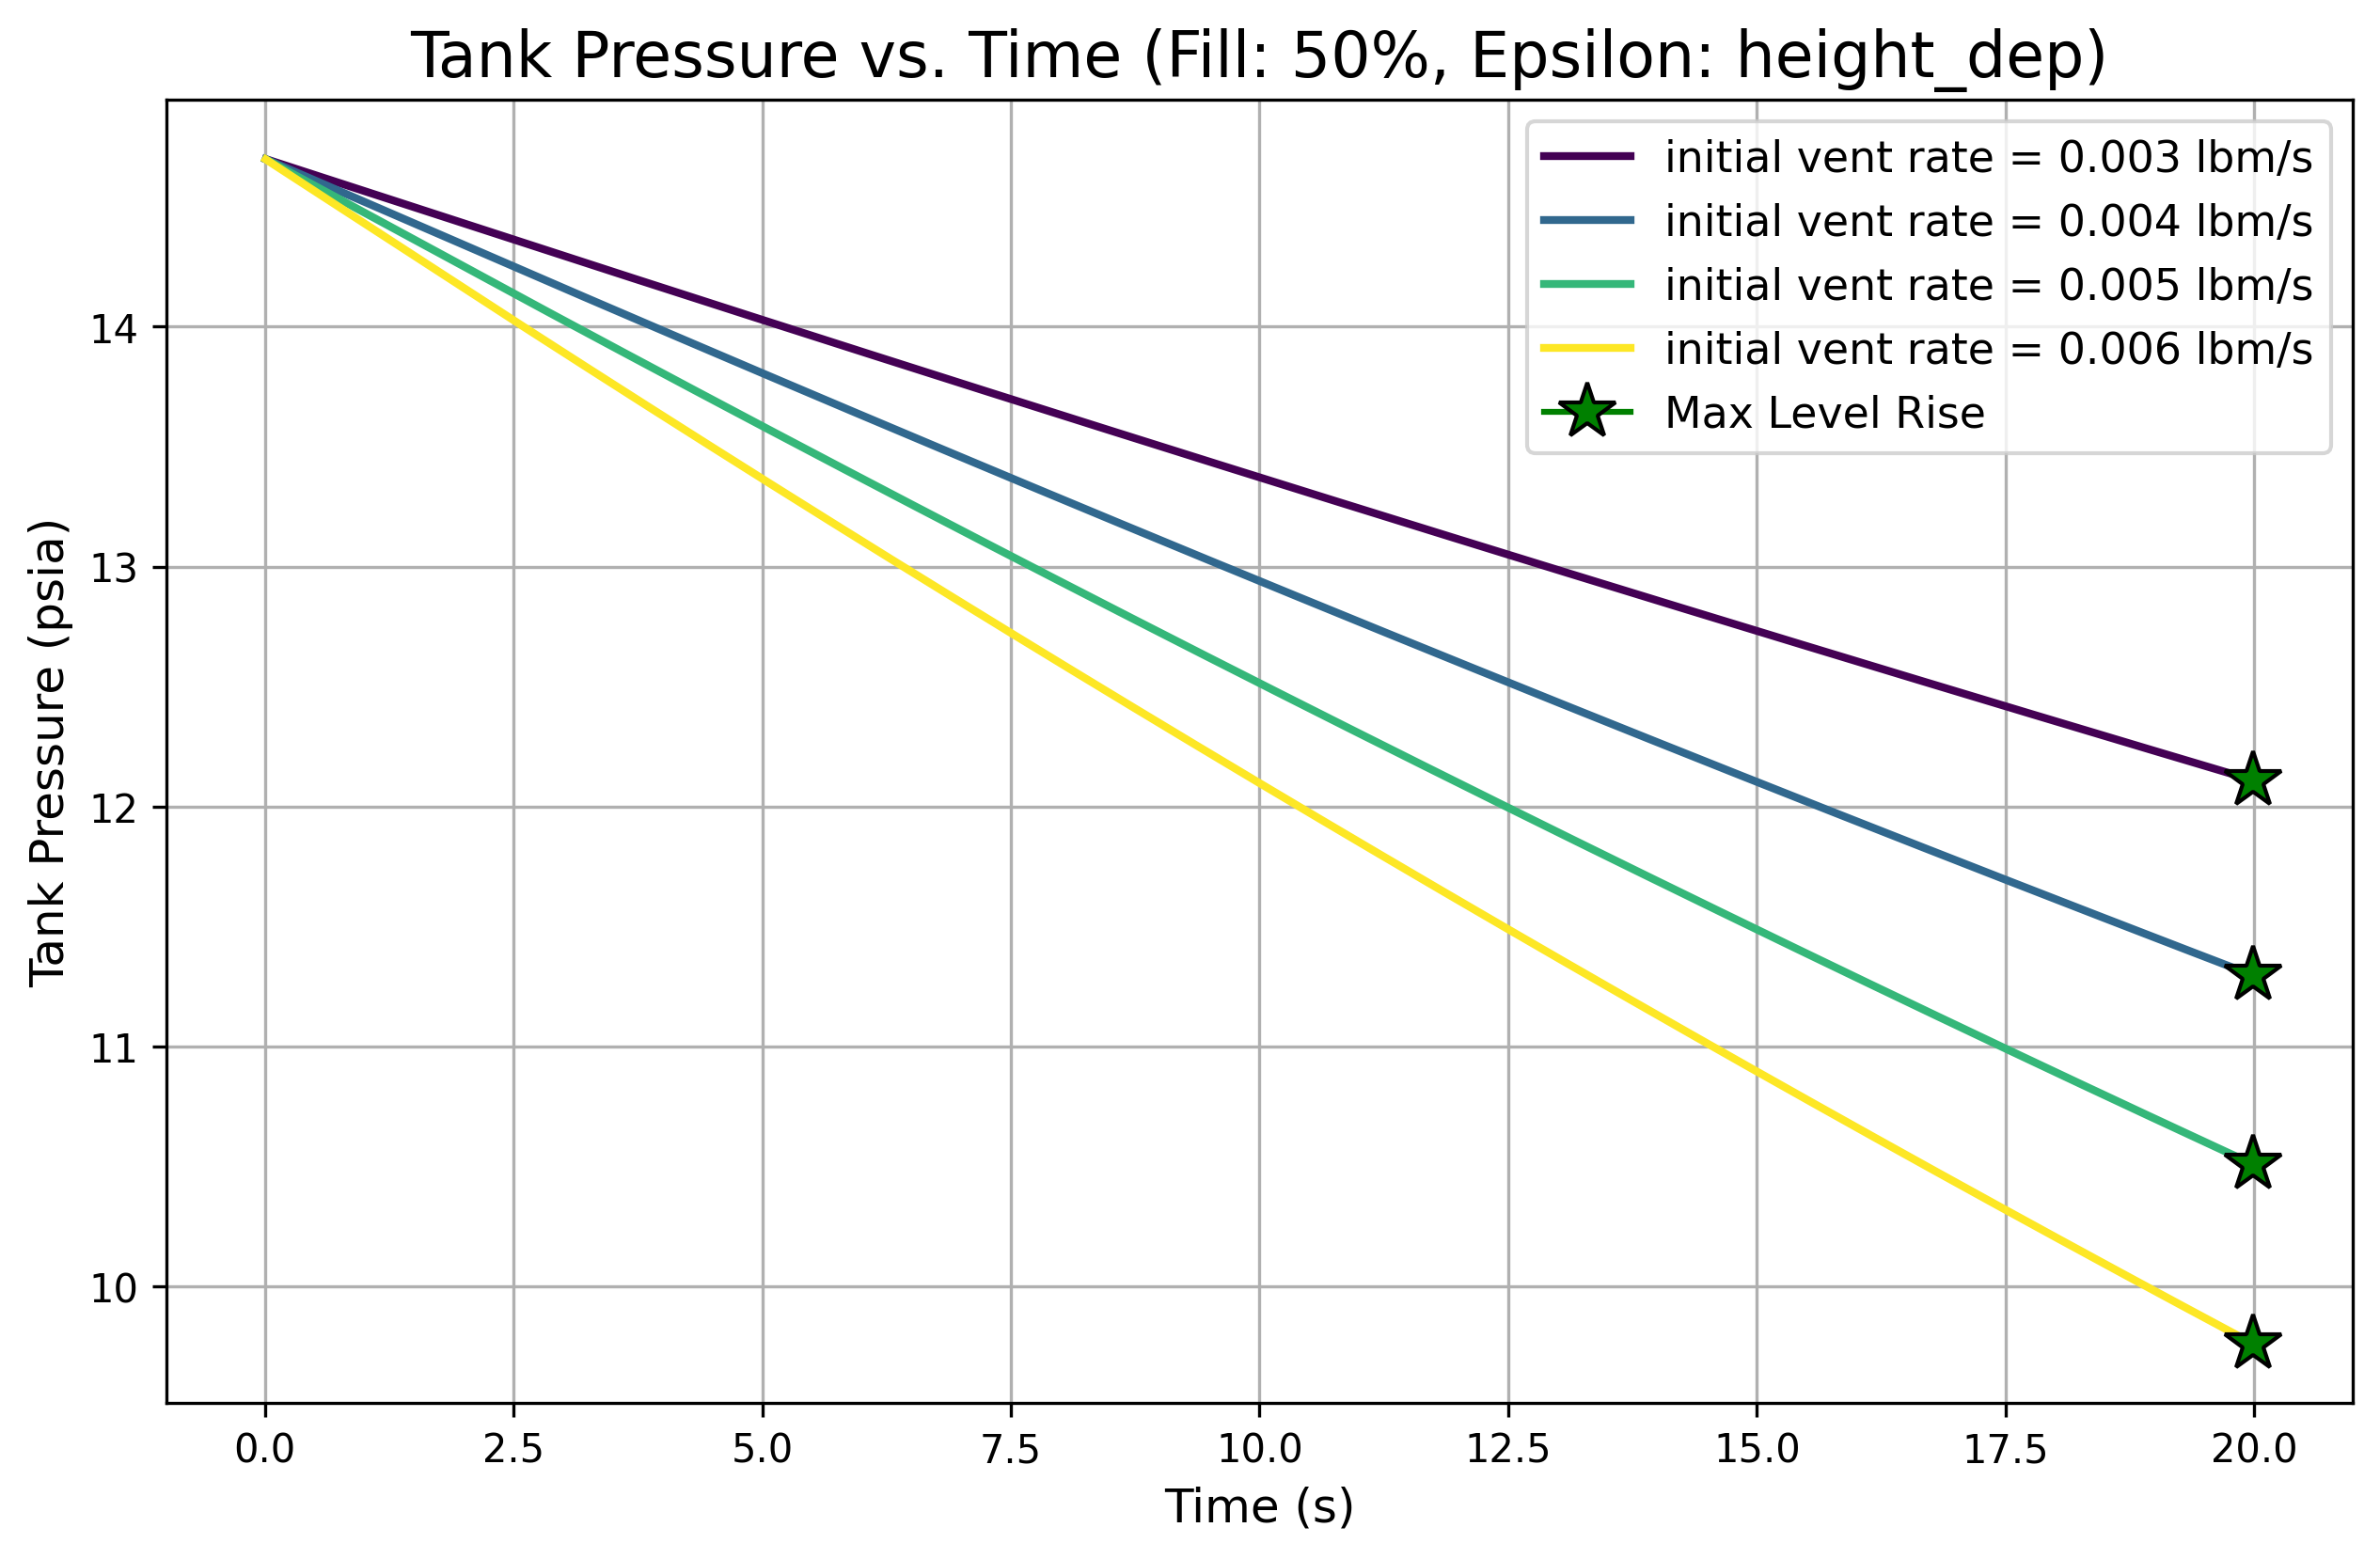
\includegraphics[width=\textwidth]{images/liqlev_0p3ftx2ft_all_vent/50_fill_pressure_height_dep.png}
        \caption{50\% Fill: Pressure}
        \label{fig:50_pressure}
    \end{subfigure}
    \hfill
    \begin{subfigure}[b]{0.48\textwidth}
        \centering
        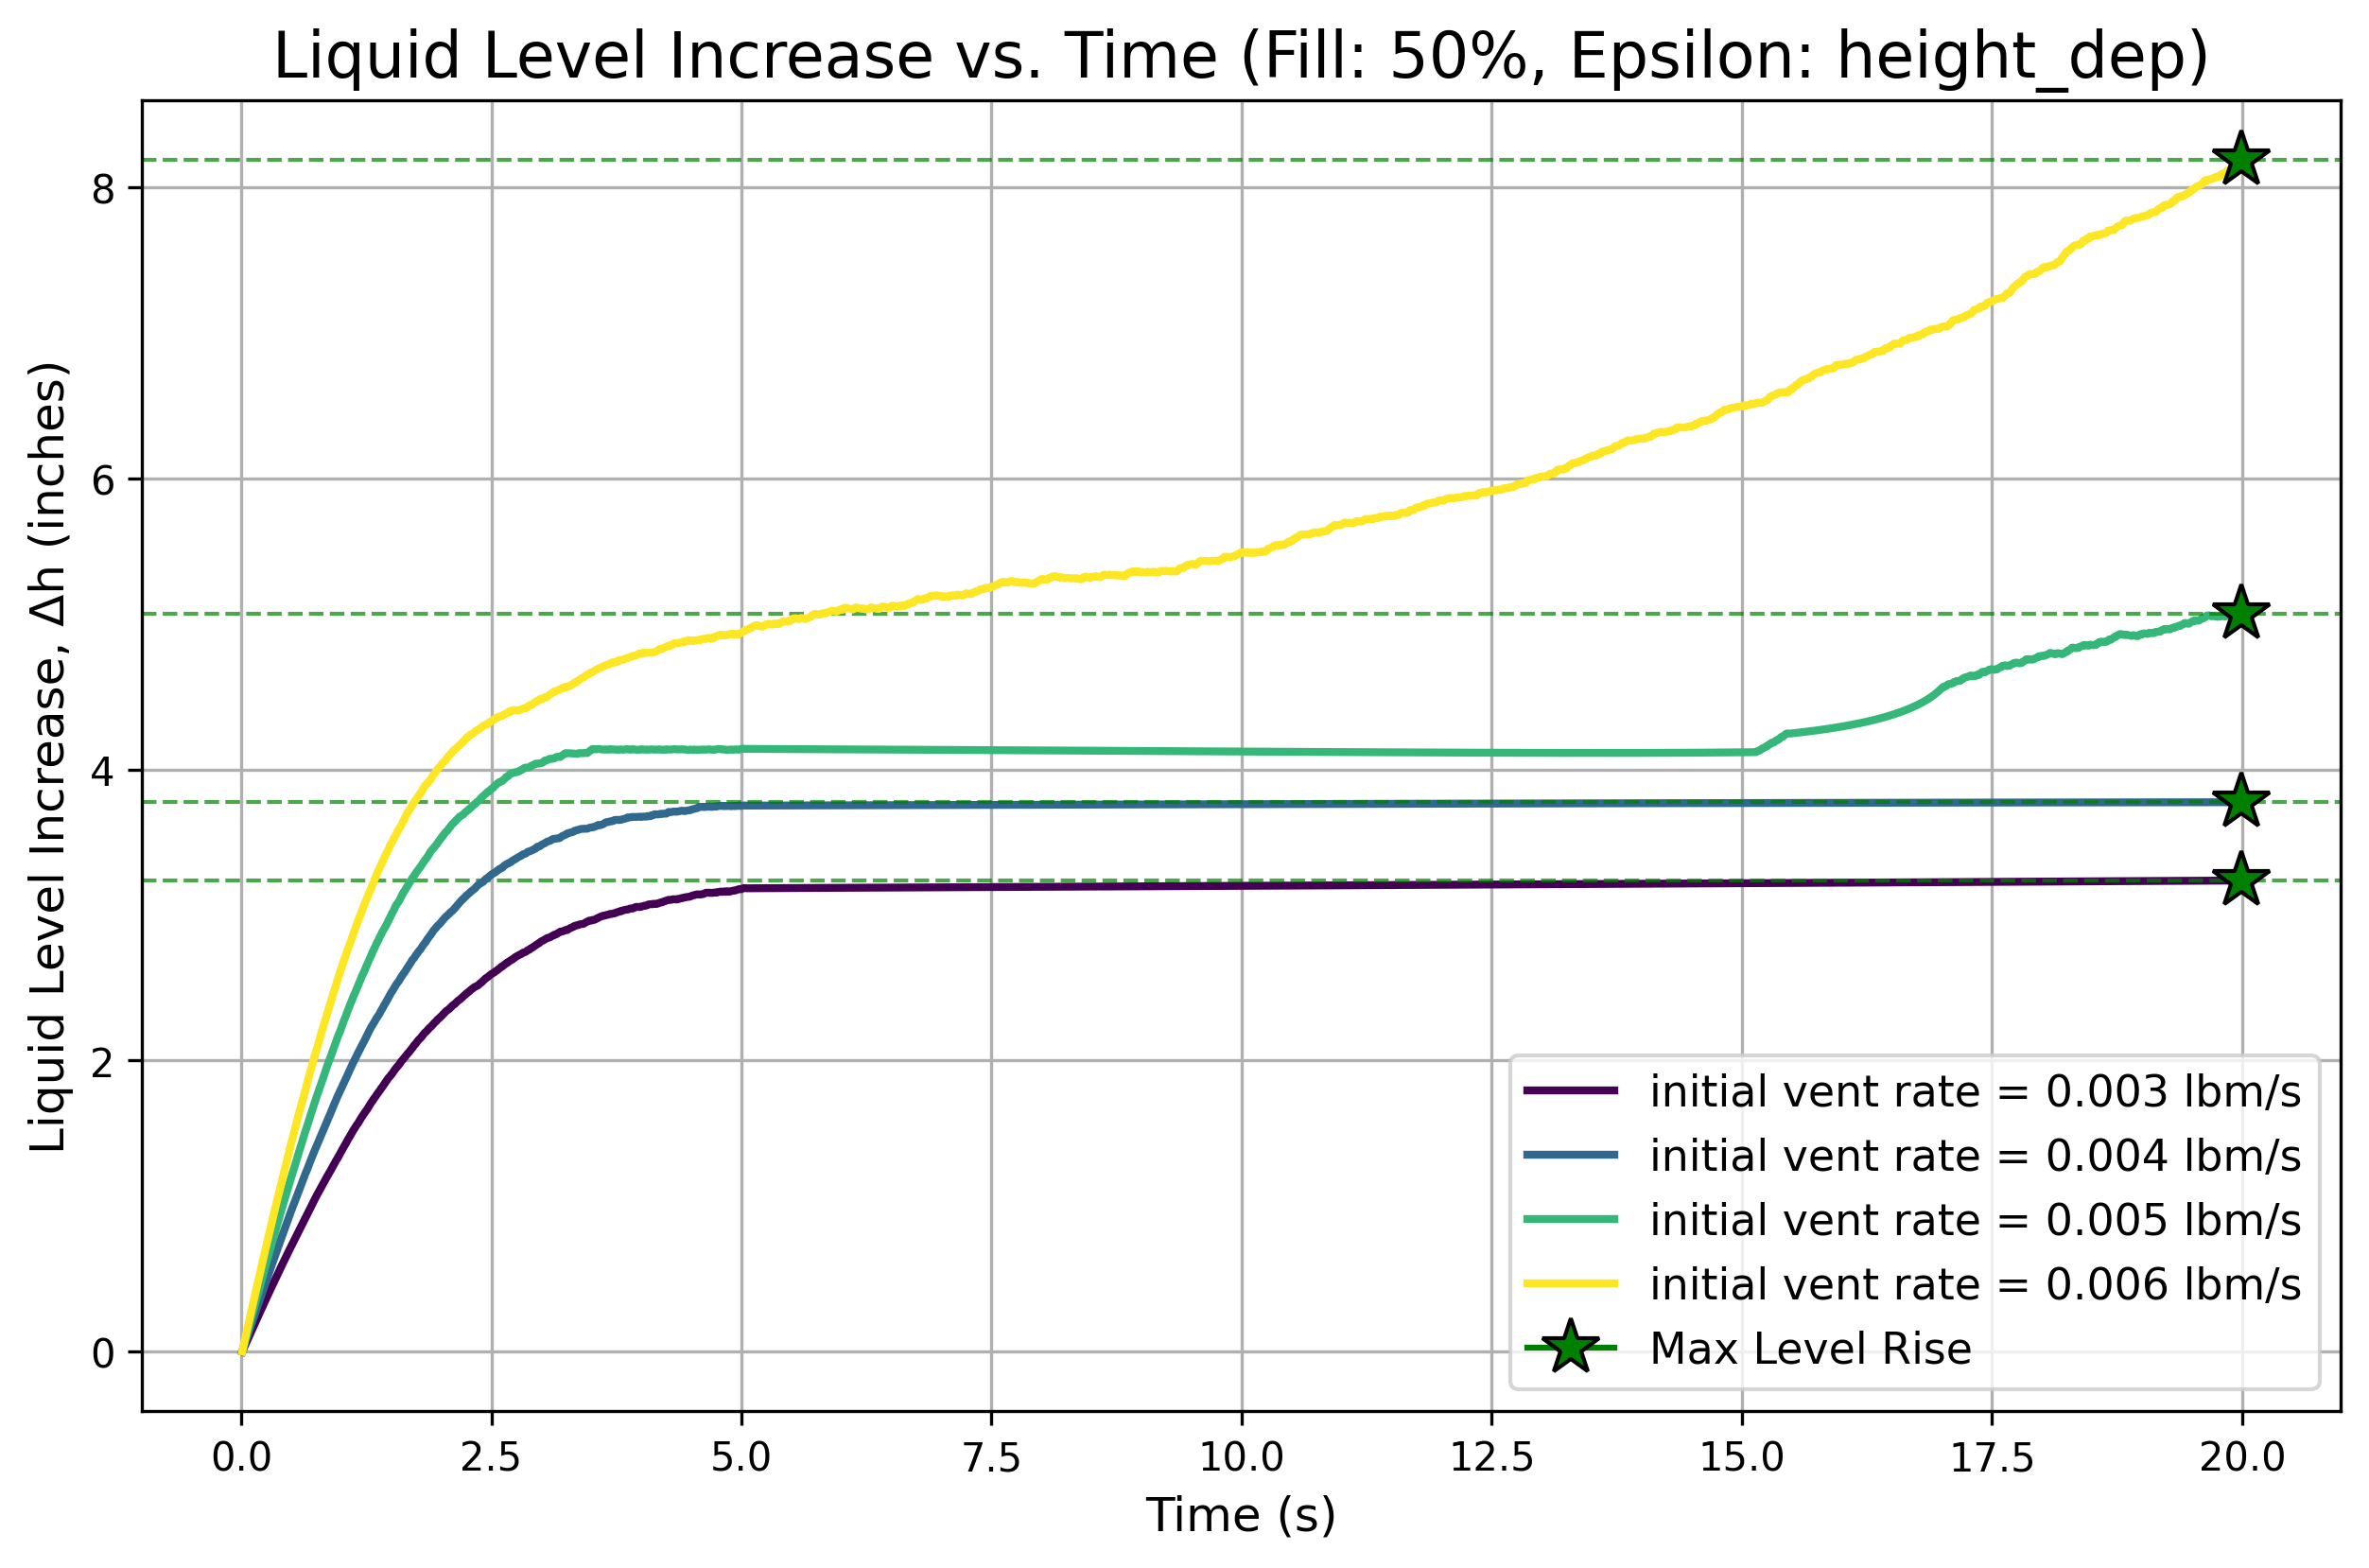
\includegraphics[width=\textwidth]{images/liqlev_0p3ftx2ft_all_vent/50_fill_liqlev_height_dep.png}
        \caption{50\% Fill: Liquid Level}
        \label{fig:50_level}
    \end{subfigure}
    
    \vspace{0.4cm}
    
    % --- Row 3: 75% Fill ---
    \begin{subfigure}[b]{0.48\textwidth}
        \centering
        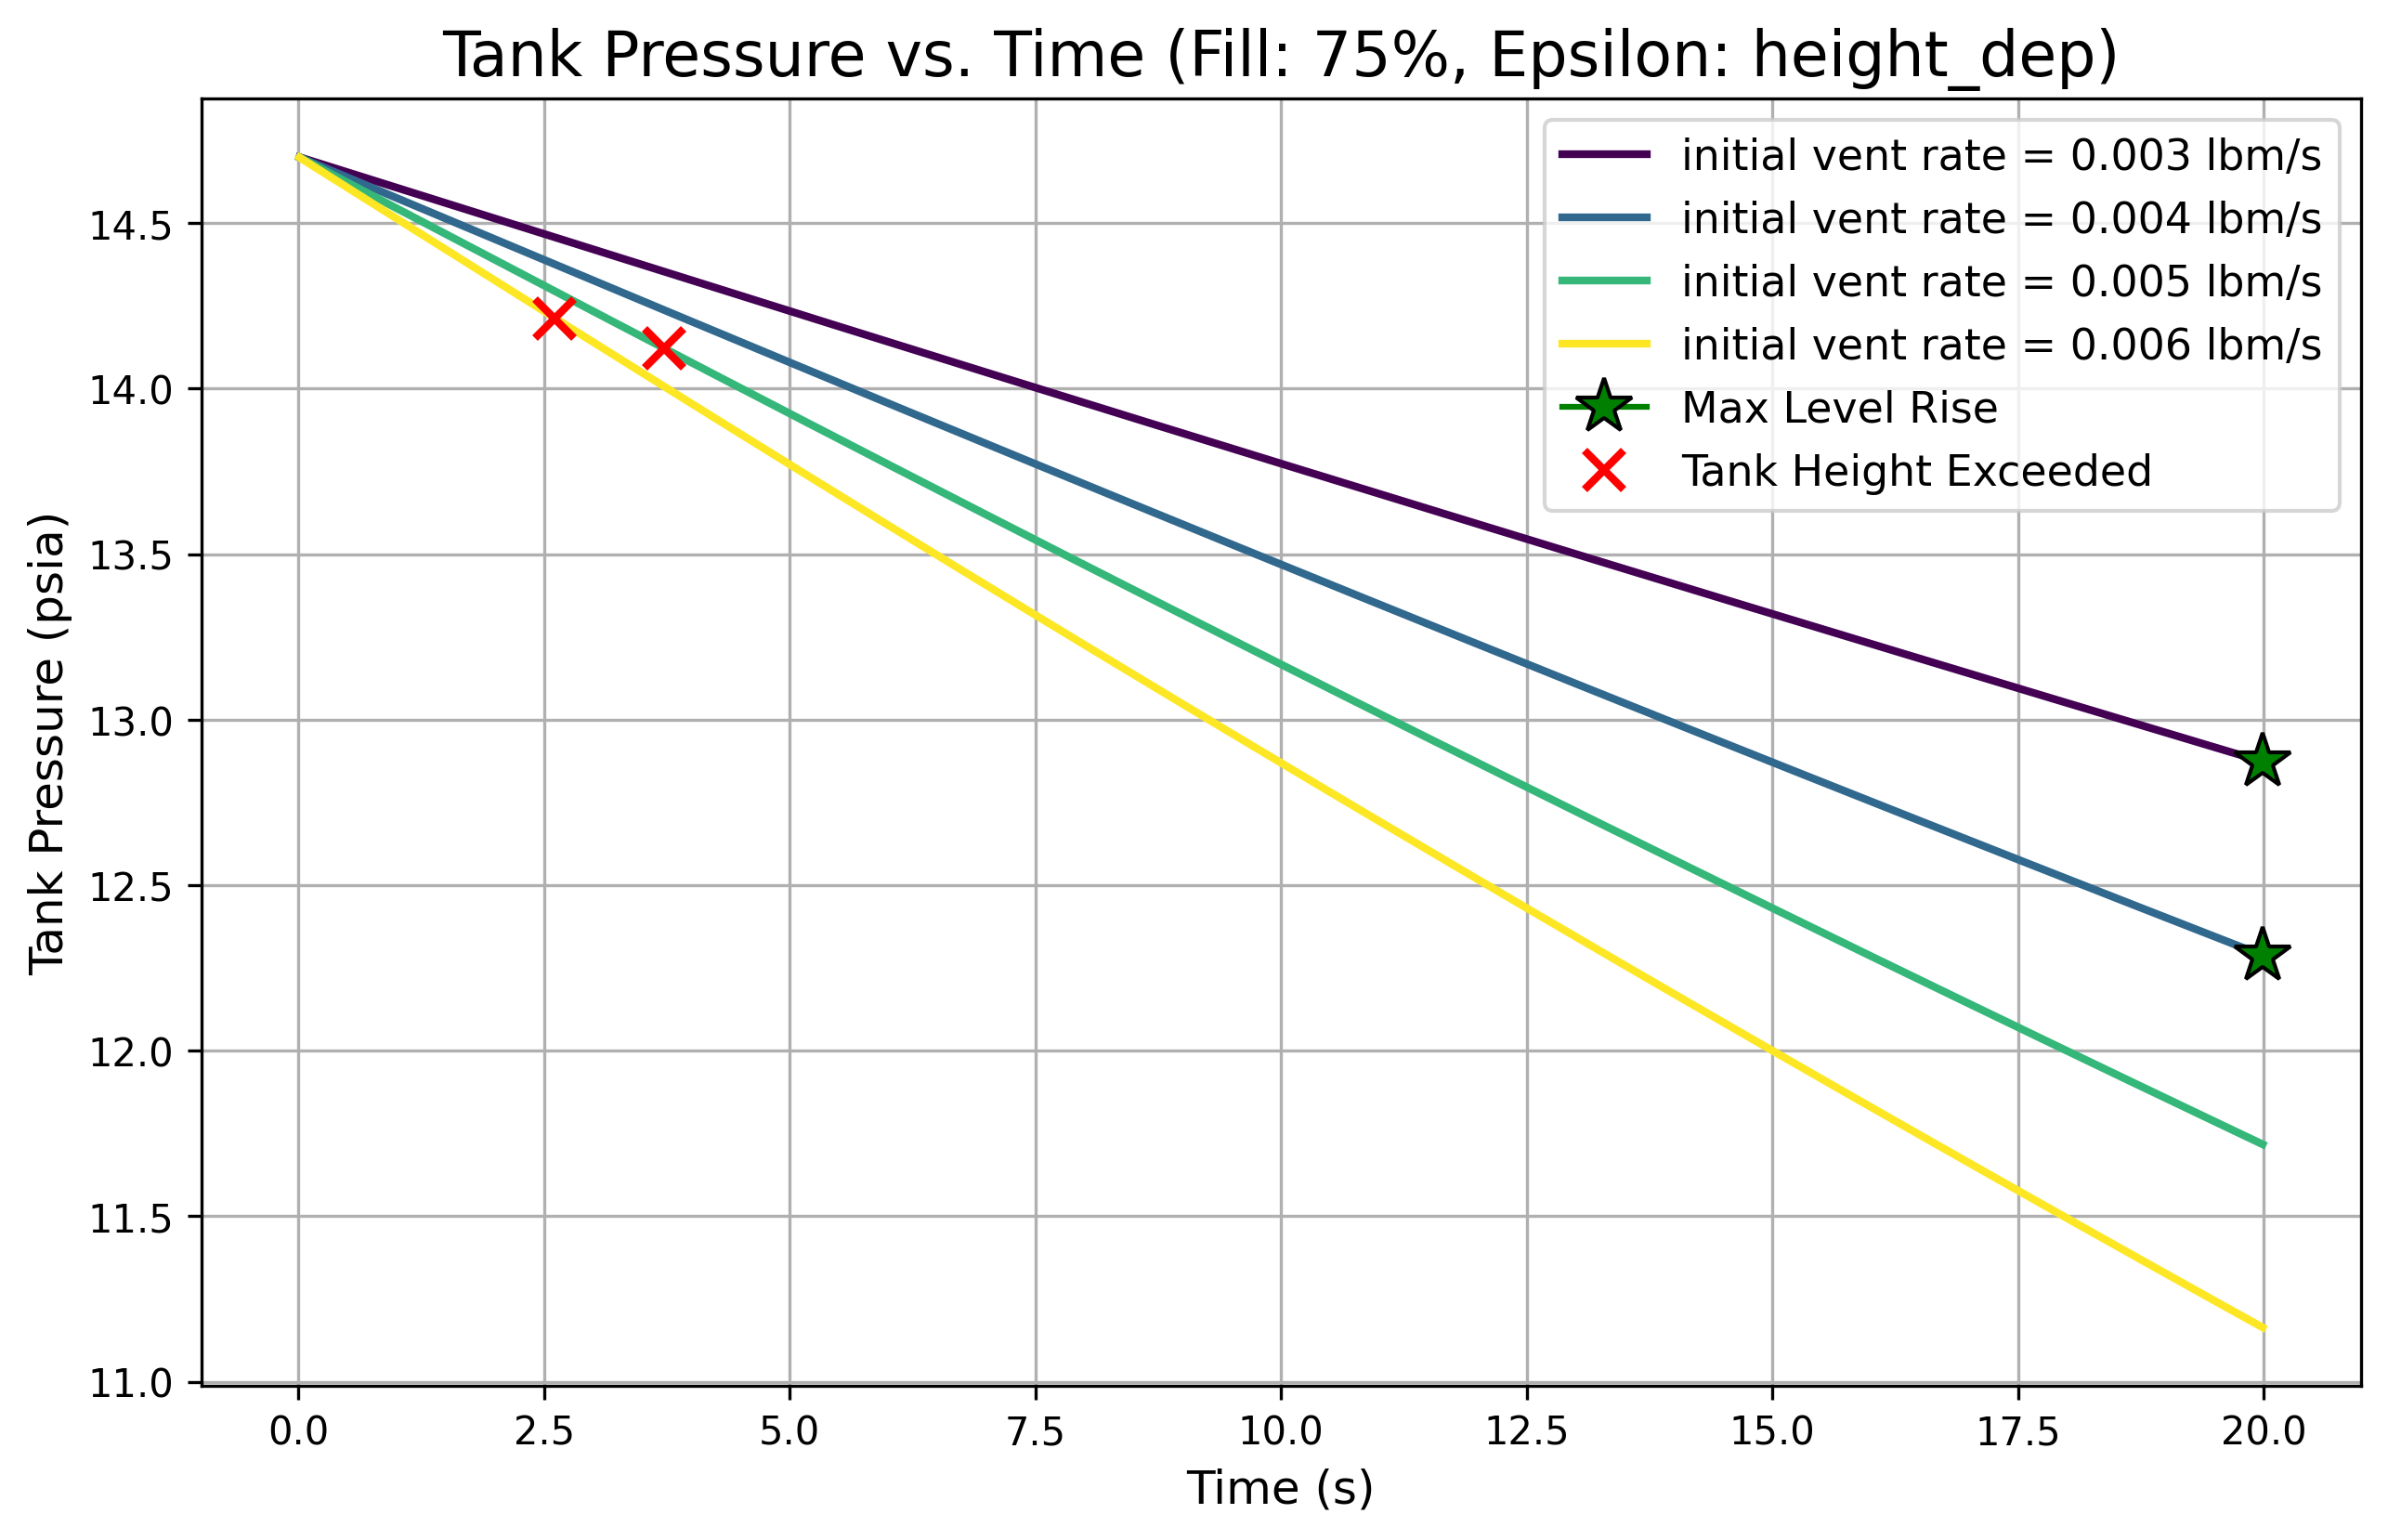
\includegraphics[width=\textwidth]{images/liqlev_0p3ftx2ft_all_vent/75_fill_pressure_height_dep.png}
        \caption{75\% Fill: Pressure}
        \label{fig:75_pressure}
    \end{subfigure}
    \hfill
    \begin{subfigure}[b]{0.48\textwidth}
        \centering
        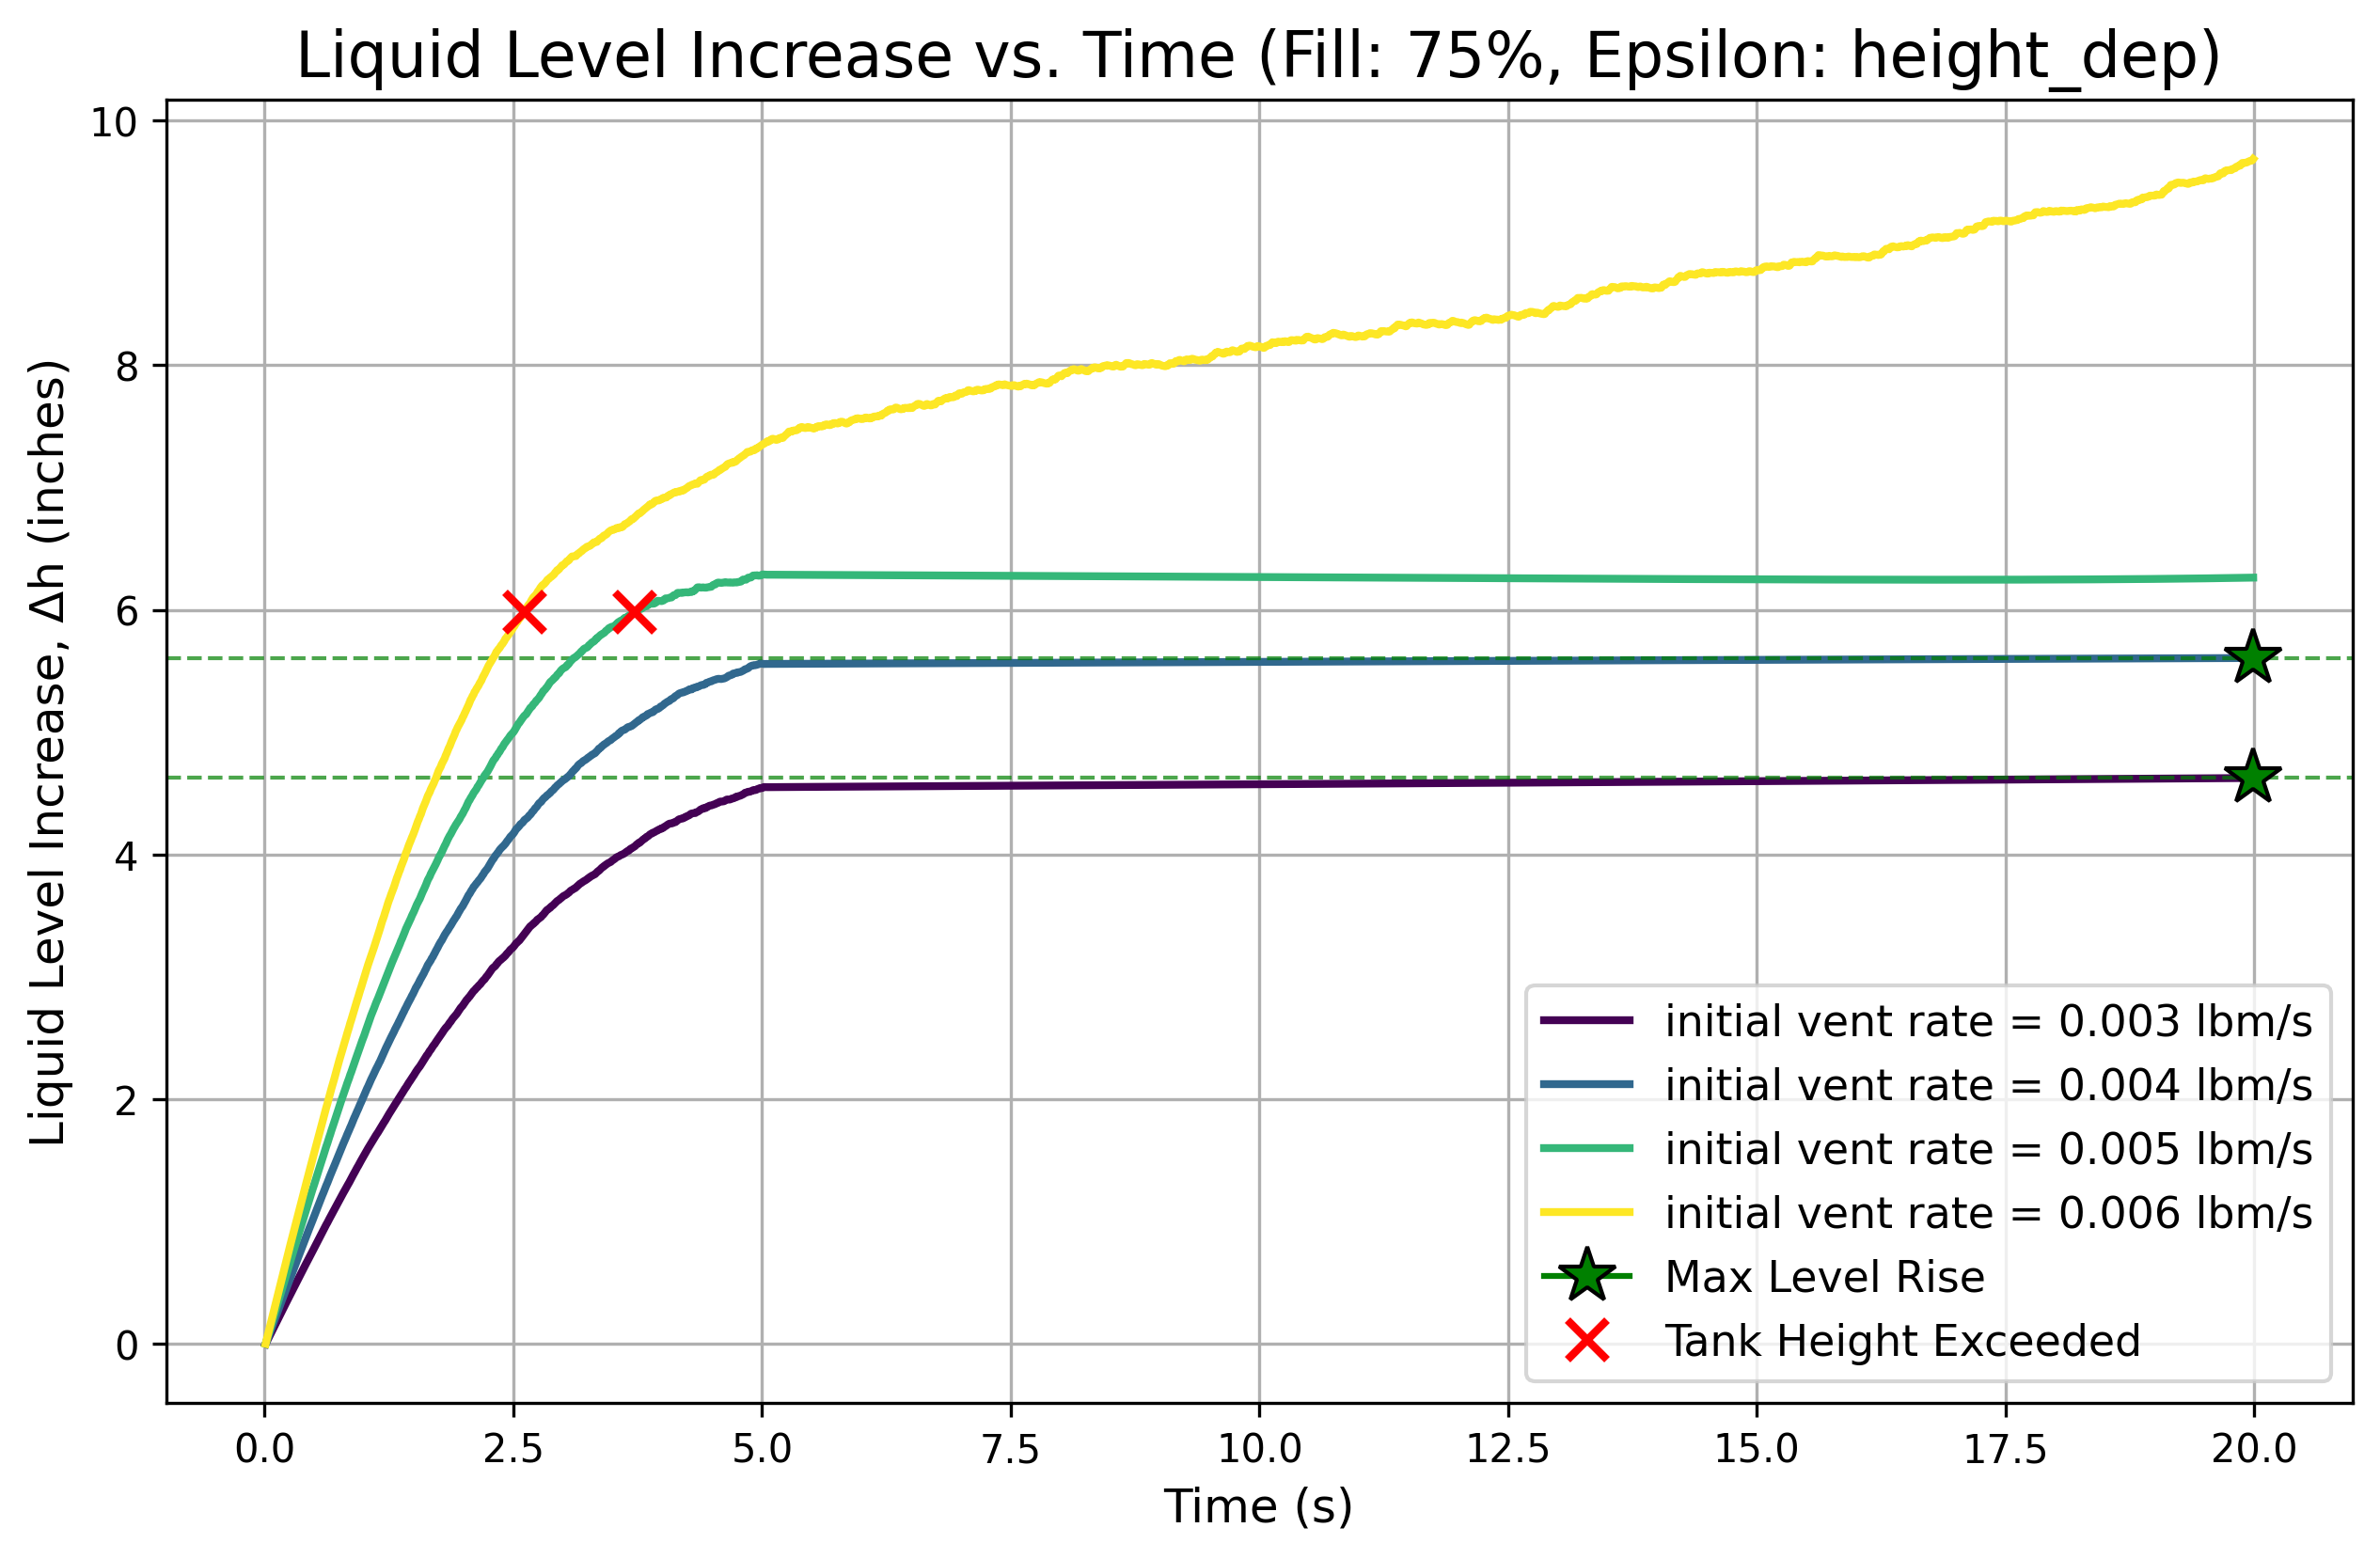
\includegraphics[width=\textwidth]{images/liqlev_0p3ftx2ft_all_vent/75_fill_liqlev_height_dep.png}
        \caption{75\% Fill: Liquid Level}
        \label{fig:75_level}
    \end{subfigure}

    \caption{Transient response of the recommended 0.3 ft diameter $\times$ 2.0 ft height tank in the 5-second facility using the height-dependent $\epsilon$ formulation. Left column: tank pressure versus time. Right column: liquid level rise (inches) versus time. Green stars denote the global maximum rise; red crosses indicate cases where the interface exceeded the tank height.}
    \label{fig:0p3ft_time_histories}
\end{figure}



\subsection{Effect of Epsilon (\texorpdfstring{$\epsilon$}{epsilon}) and Model Sensitivity}
The boil-off partitioning parameter $\epsilon$ represents the instantaneous fraction of total vapor mass generated within the wall thermal boundary layer relative to the vapor generated at the liquid-vapor free surface. In the modernized Python implementation of LIQLEV, $\epsilon$ is evaluated at every solver time step. When operating in the default height-dependent mode (neps = 0), it is computed directly from the geometric wetted-area ratio according to the Moran formulation:

\[
\epsilon(t) = \frac{\pi D \, h(t)}{\pi D \, h(t) + \frac{\pi D^{2}}{4}},
\]

where $D$ is the tank diameter and $h(t)$ is the instantaneous liquid height. This expression assumes that the rate of vapor production scales proportionally with the respective heat-transfer areas (sidewall wetted surface versus free interface).

A dedicated sensitivity study quantified the dominant influence of $\epsilon$ at low gravity levels. The time-dependent $\epsilon(t)$ schedule derived from the evolving wetted-area ratio produces physically representative liquid level rise behavior. When this dynamic schedule was compared against constant-$\epsilon$ cases ($\epsilon = 0.4$, $0.625$, and $0.8$) under identical tank geometry, initial fill fraction, and vent rate, peak liquid level rise differed by up to 30--40\,\%. The effect is most pronounced under $10^{-5}$\,g conditions, where reduced buoyancy allows wall-generated vapor bubbles to remain entrained longer, thereby increasing the volumetric displacement of the bulk liquid column. These differences, as well as the temporal evolution of $\epsilon(t)$ itself, are clearly illustrated in the dedicated epsilon-sensitivity time-history and contour plots compiled for each reduced-gravity facility.

\subsection{JAXA Validation and Code Verification}
Model fidelity was verified through direct comparison with the JAXA $30\,m^3$ LH$_2$ large-scale venting experiment reported by Tani et al.~\cite{tani2021pressure}. The dedicated validation module \texttt{tani\_validation.py} accurately reproduced the experimentally derived piecewise-cubic vent mass-flow profile (rapid stepped blowdown over the initial $0$--$15$\,s followed by long-term decay), shown in Figure~\ref{fig:jaxa_vent_profile}.

\begin{figure}[htbp]
\centering
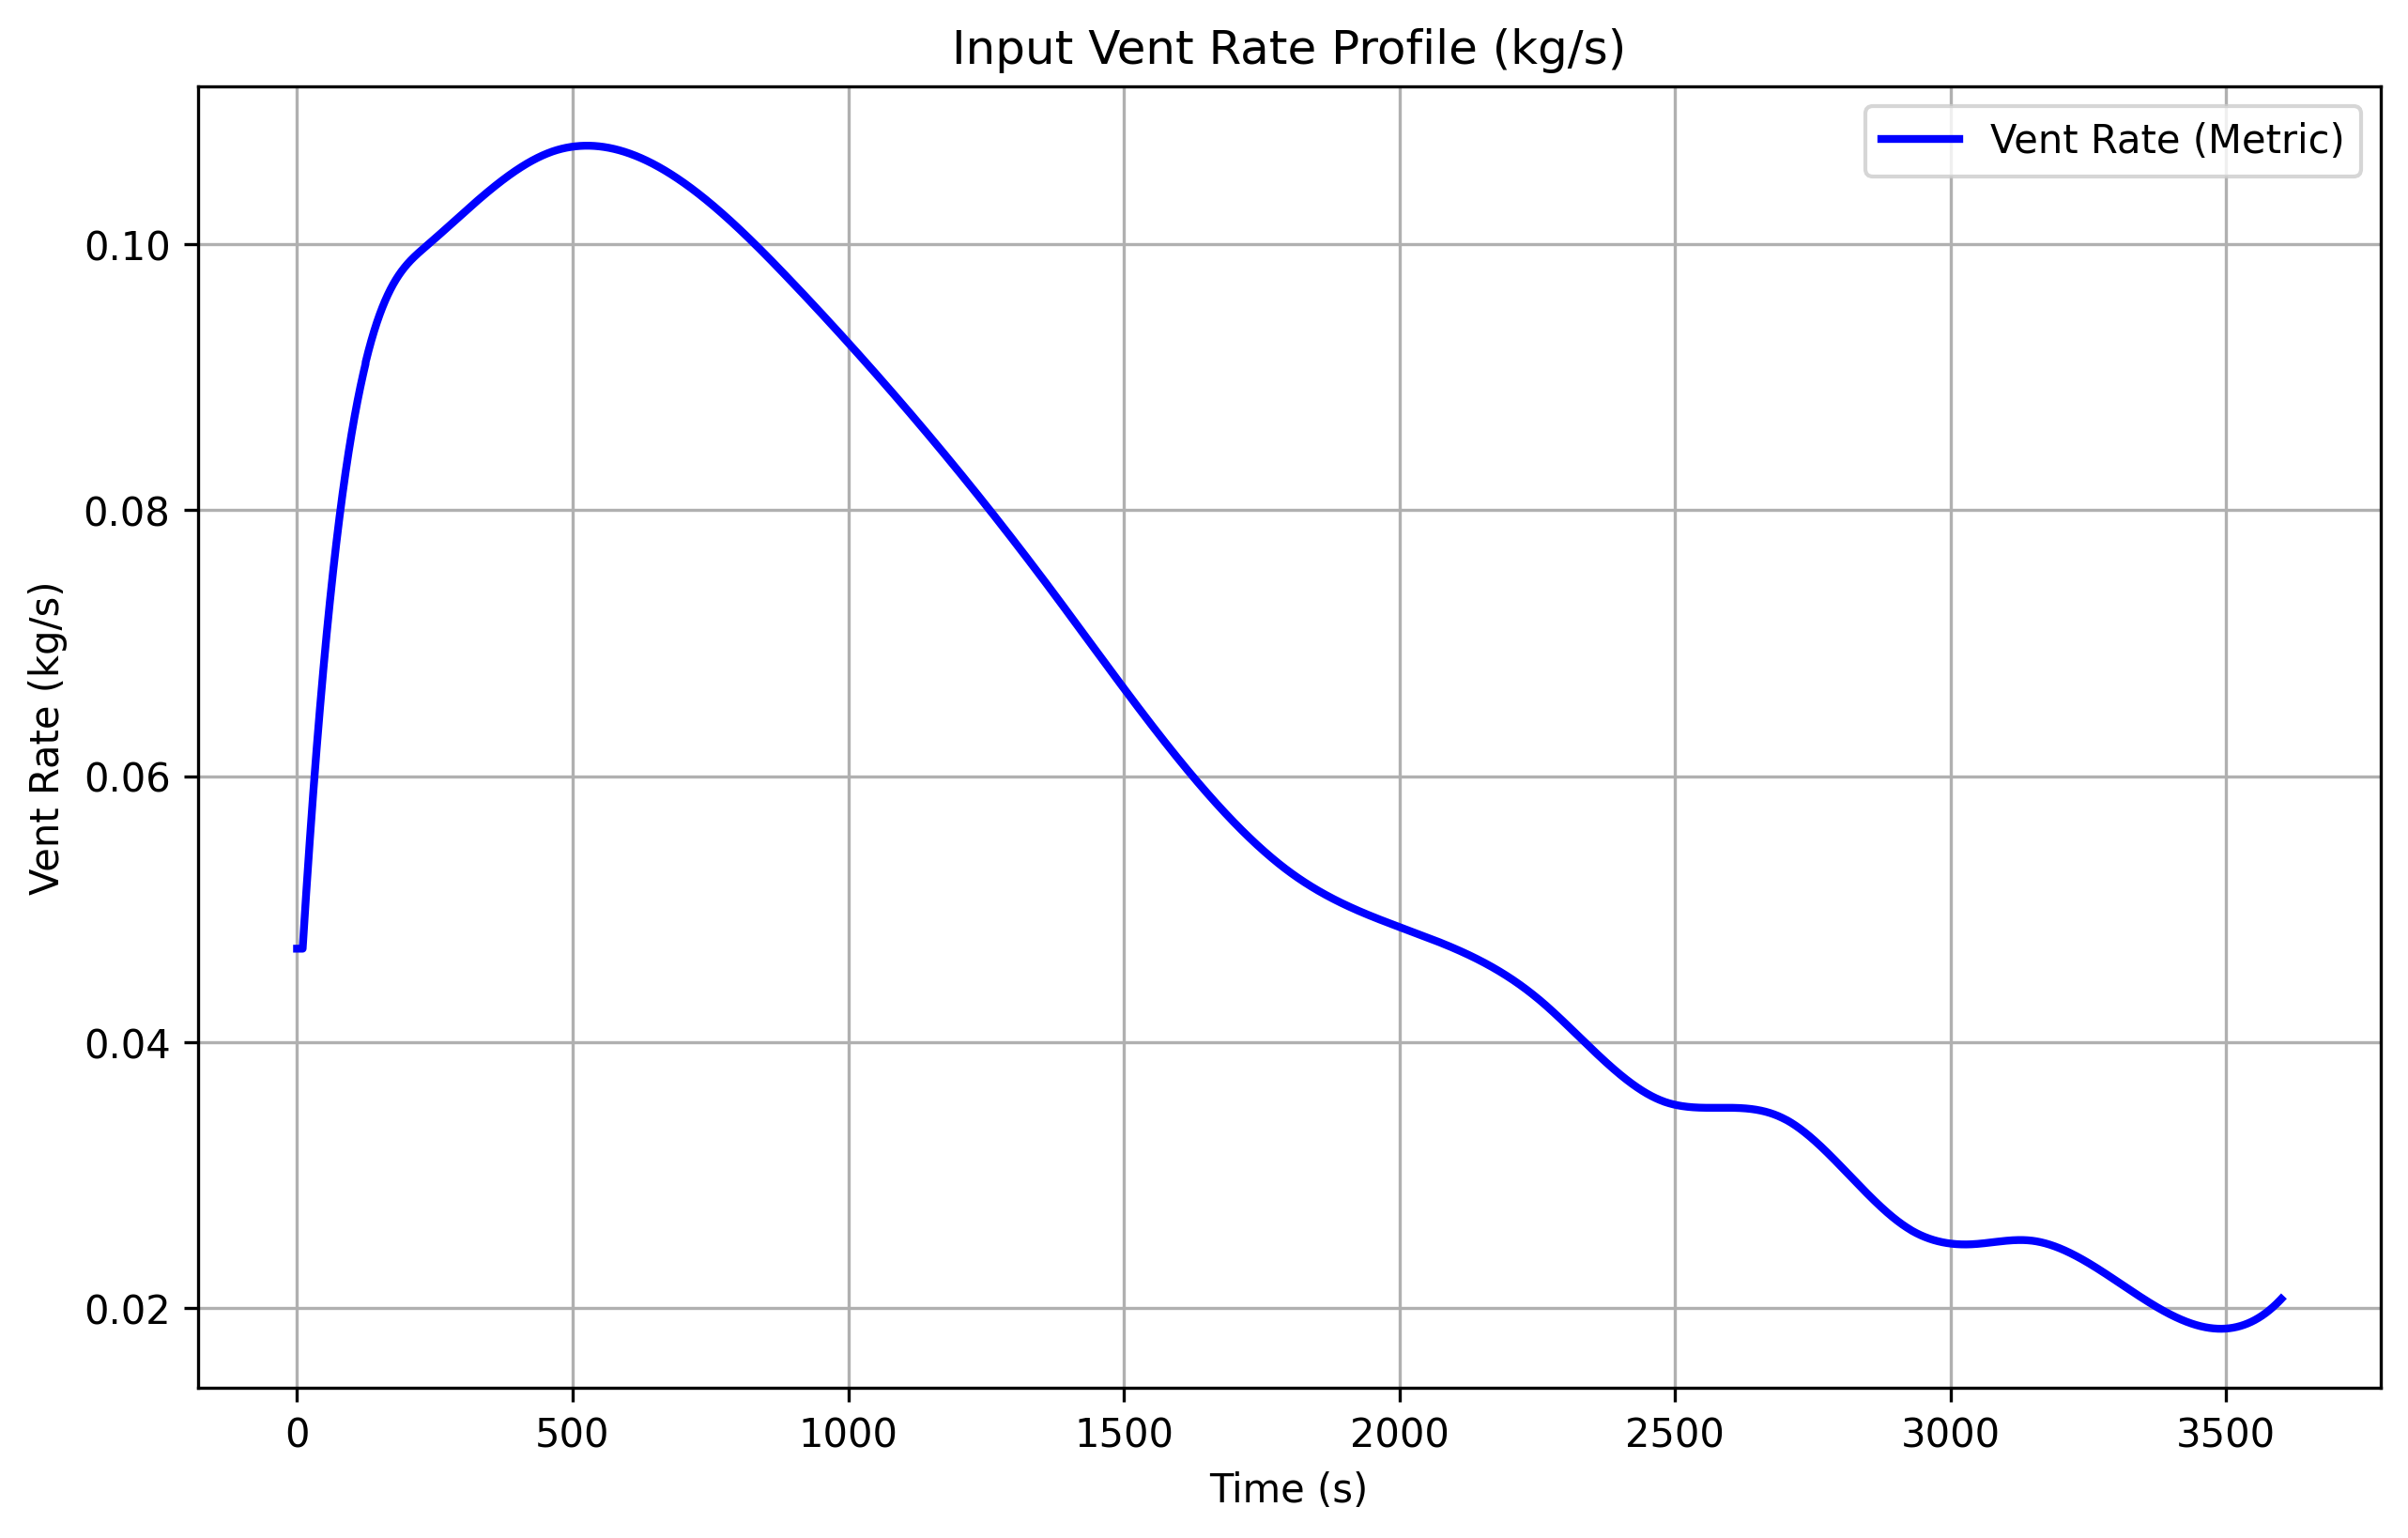
\includegraphics[width=0.95\textwidth]{images/tani_validation/vent_rate.png}
\caption{Input vent-rate profile (kg/s) used for JAXA validation. The piecewise-cubic fit reproduces the rapid stepped blowdown (0--15\,s) followed by long-term decay, closely matching the experimental data.}
\label{fig:jaxa_vent_profile}
\end{figure}

When exercised with the standard height-dependent $\epsilon$ formulation ($\epsilon(t) = \frac{\pi D h(t)}{\pi D h(t) + \pi D^2/4}$), the model significantly under-predicted both the initial vapor generation rate and the measurable liquid level rise. This discrepancy arises because, in the large-volume JAXA tank ($V=30\,m^3$, $D=2.3$\,m) at a high fill fraction ($\approx 82$\,\%), the dominant vapor production mechanism during rapid depressurization is distributed bulk flashing and volumetric boiling throughout the entire superheated liquid column, rather than being confined to the thin thermal boundary layer along the wetted sidewall.

To reproduce the experimentally observed dynamics, a high effective $\epsilon$ was introduced via a ``bulk\_fake'' mode (constant $\epsilon \approx 50$). Physically, an $\epsilon$ value of 50 means that the model treats the effective vapor-generating surface area as 50 times larger than the actual wetted sidewall area—equivalent to scaling the available liquid volume that participates in boiling by the same factor to emulate the dominant bulk-boiling contribution.

The resulting pressure decay predictions for different $\epsilon$ modes are shown in Figure~\ref{fig:jaxa_pressure}. The bulk\_fake modes (especially $\epsilon=50$ and $75$) show close agreement with the experimental data points, correctly capturing the initial pressure recovery caused by delayed bulk boiling and the subsequent near-equilibrium depressurization. In contrast, the height-dependent mode under-predicts the early vapor generation rate; its curve is largely obscured behind the $\epsilon=1.0$ line and is therefore not visible on the plot.

\begin{figure}[htbp]
\centering
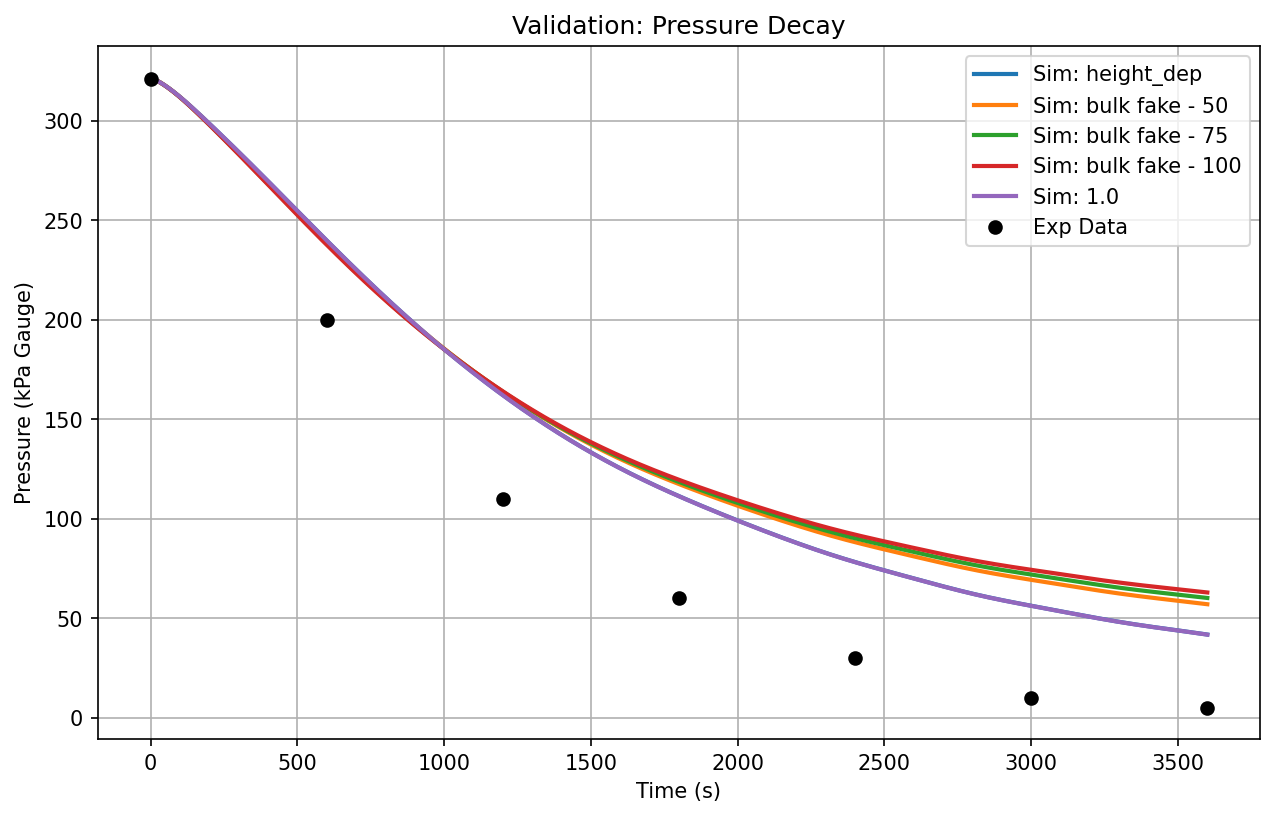
\includegraphics[width=0.95\textwidth]{images/tani_validation/pressure_decay_full.png}
\caption{Comparison of simulated ullage pressure decay versus experimental data for the JAXA $30\,m^3$ LH$_2$ test. Bulk\_fake modes ($\epsilon=50$, $75$, $100$) show close agreement with the data, while the height-dependent mode under-predicts the initial vapor generation (its curve lies behind the $\epsilon=1.0$ line and is not visible).}
\label{fig:jaxa_pressure}
\end{figure}

The liquid level rise predictions (Figure~\ref{fig:jaxa_level}) further confirm the necessity of the bulk\_fake adjustment. The height-dependent mode produces only a modest rise, whereas the bulk\_fake modes reach the experimentally observed displacement. This rise was detected when only the TIE-04 temperature probe (located at 6.422\,m from the tank bottom) became wetted. With an initial liquid height of 6.248\,m, this corresponds to an interface displacement of $0.174$\,m ($\approx 6.85$\,inches or $17.4$\,cm) within the first few seconds. The $\epsilon=50$ case matches this experimental rise most closely.

\begin{figure}[htbp]
\centering
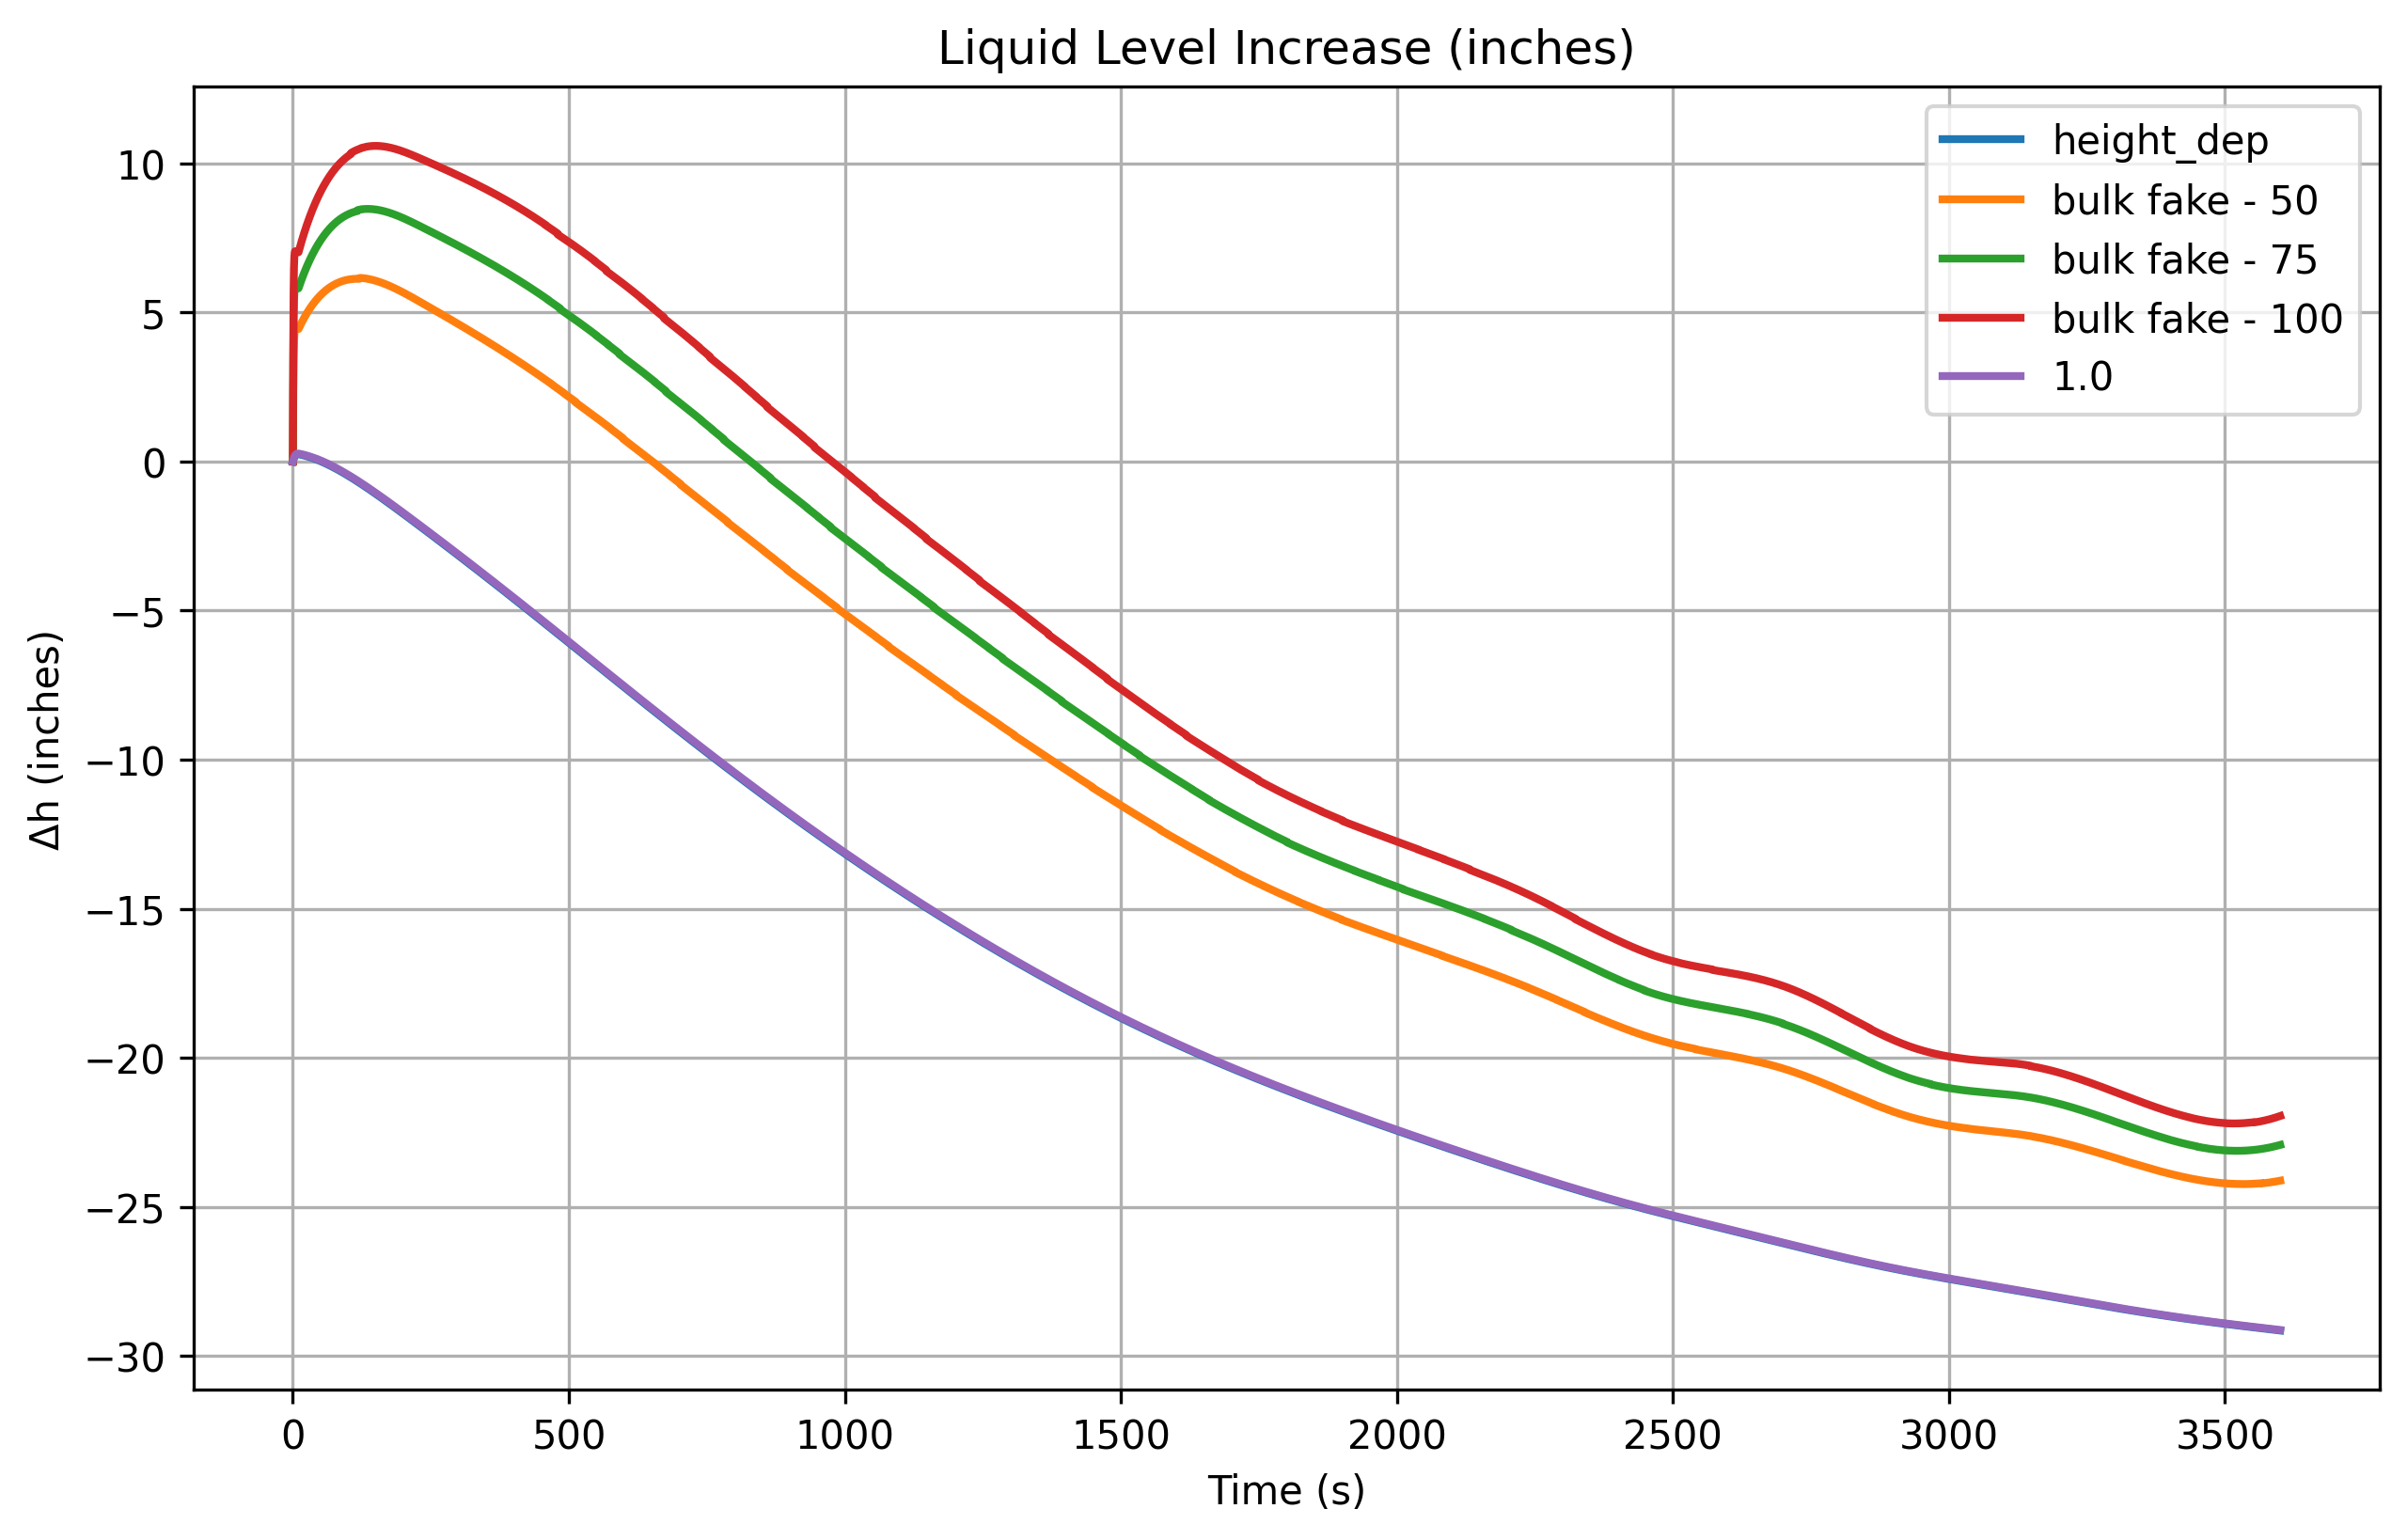
\includegraphics[width=0.95\textwidth]{images/tani_validation/liqlev_full.png}
\caption{Liquid level rise (inches) versus time for different $\epsilon$ modes in the JAXA validation case. Only the bulk\_fake modes reproduce the experimentally observed $\approx 6.85$-inch rise.}
\label{fig:jaxa_level}
\end{figure}

These results confirm that the migration to \texttt{CoolProp} for high-accuracy real-fluid properties, combined with dynamic time-stepping and flexible $\epsilon$ modeling, eliminated the numerical artifacts of the legacy VBA implementation. The bulk\_fake mode (high constant $\epsilon$) provides a practical and effective engineering approximation for large tanks in which bulk boiling dominates. However, future development should incorporate an explicit bulk-liquid boiling source term in addition to the original wall boundary-layer formulation. When the classical boundary-layer foundation is augmented with a physically based bulk contribution, the model will remain a robust and accurate engineering tool for cryogenic venting predictions across the full range of tank scales.


\subsection{Computational Cross-Validation via Multiphase CFD}
To assess the validity of the one-dimensional interface displacement assumptions underlying the LIQLEV boundary-layer model, a hybrid analytical--CFD cross-validation study was conducted using three-dimensional multiphase computational fluid dynamics (CFD) in ANSYS Fluent. The Volume-of-Fluid (VOF) method was employed to track the liquid-vapor interface evolution under reduced gravity.

A one-way coupling strategy was adopted to isolate hydrodynamic displacement effects while circumventing the modeling uncertainties of full heat transfer and phase-change physics. The transient vapor mass generation rate $\dot{m}_{\rm vapor}(t)$ (boundary-layer plus interface contributions) computed by the LIQLEV model was exported and prescribed as a time-dependent vapor mass inlet boundary condition through a small orifice located on the bottom wall of the cylindrical domain. This approach accurately reproduces the net volumetric addition arising from wall boundary-layer boil-off without requiring an energy equation or detailed nucleation modeling in the CFD solver.

The representative simulation utilized a 0.3\,ft diameter $\times$ 2.0\,ft height cylindrical tank at an initial 50\,\% liquid fill fraction, subject to the gravity profile recorded during past NASA GRC 5-second zero-gravity facility experiments. High-resolution prism inflation layers were applied along the tank walls to resolve the near-wall liquid climb, and surface tension effects were captured using the continuum surface force (CSF) model. The SST $k$-$\omega$ turbulence model was employed with a fixed time step of 0.001\,s for a total simulation duration of 5\,s.

The LIQLEV-predicted liquid level rise for this configuration at the lowest vent rate (0.003\,lbm/s) is shown in Figure~\ref{fig:liqlev_time_history}. The model predicts a smooth rise that reaches its maximum of approximately 3.2 inches well within the 5-second low-gravity window.

\begin{figure}[htbp]
\centering
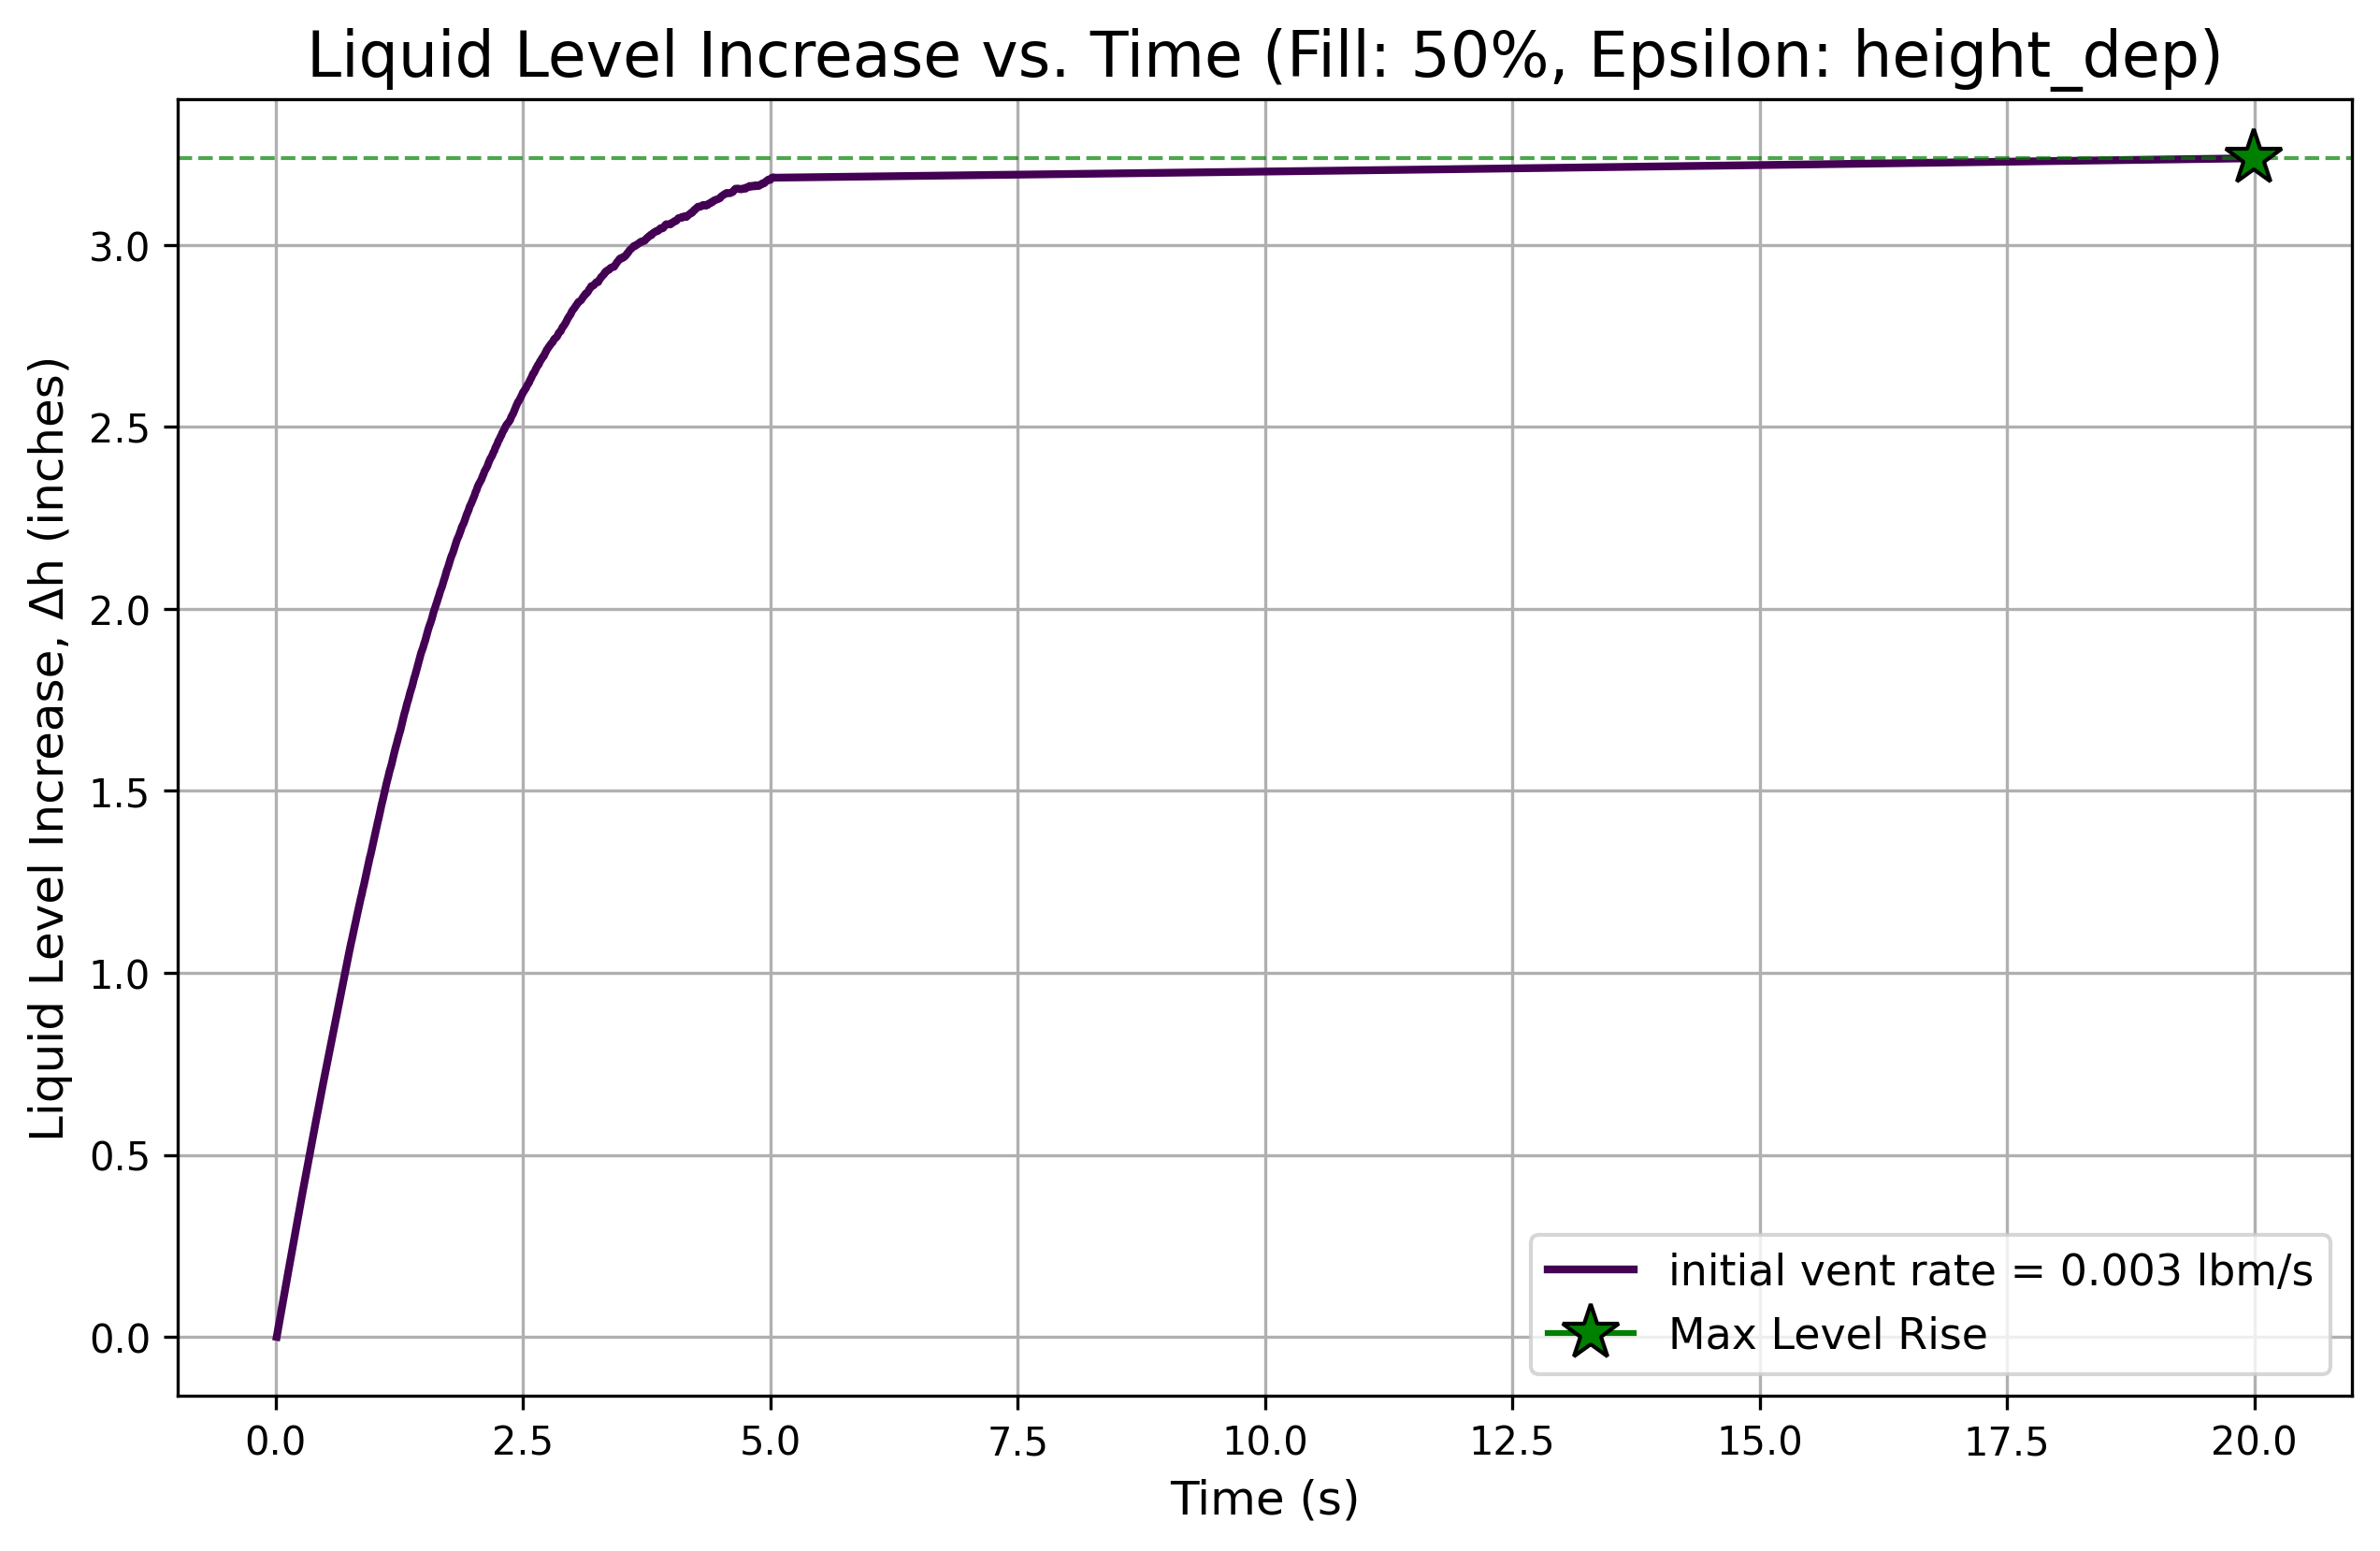
\includegraphics[width=0.95\textwidth]{images/0p003.png}
\caption{LIQLEV-predicted liquid level rise versus time for the 0.3\,ft diameter $\times$ 2.0\,ft height tank at 50\,\% fill fraction and 0.003\,lbm/s vent rate (height-dependent $\epsilon$ formulation). The green star marks the global maximum rise.}
\label{fig:liqlev_time_history}
\end{figure}

\begin{figure}[htbp]
\centering

\begin{subfigure}[b]{0.95\textwidth}
\centering
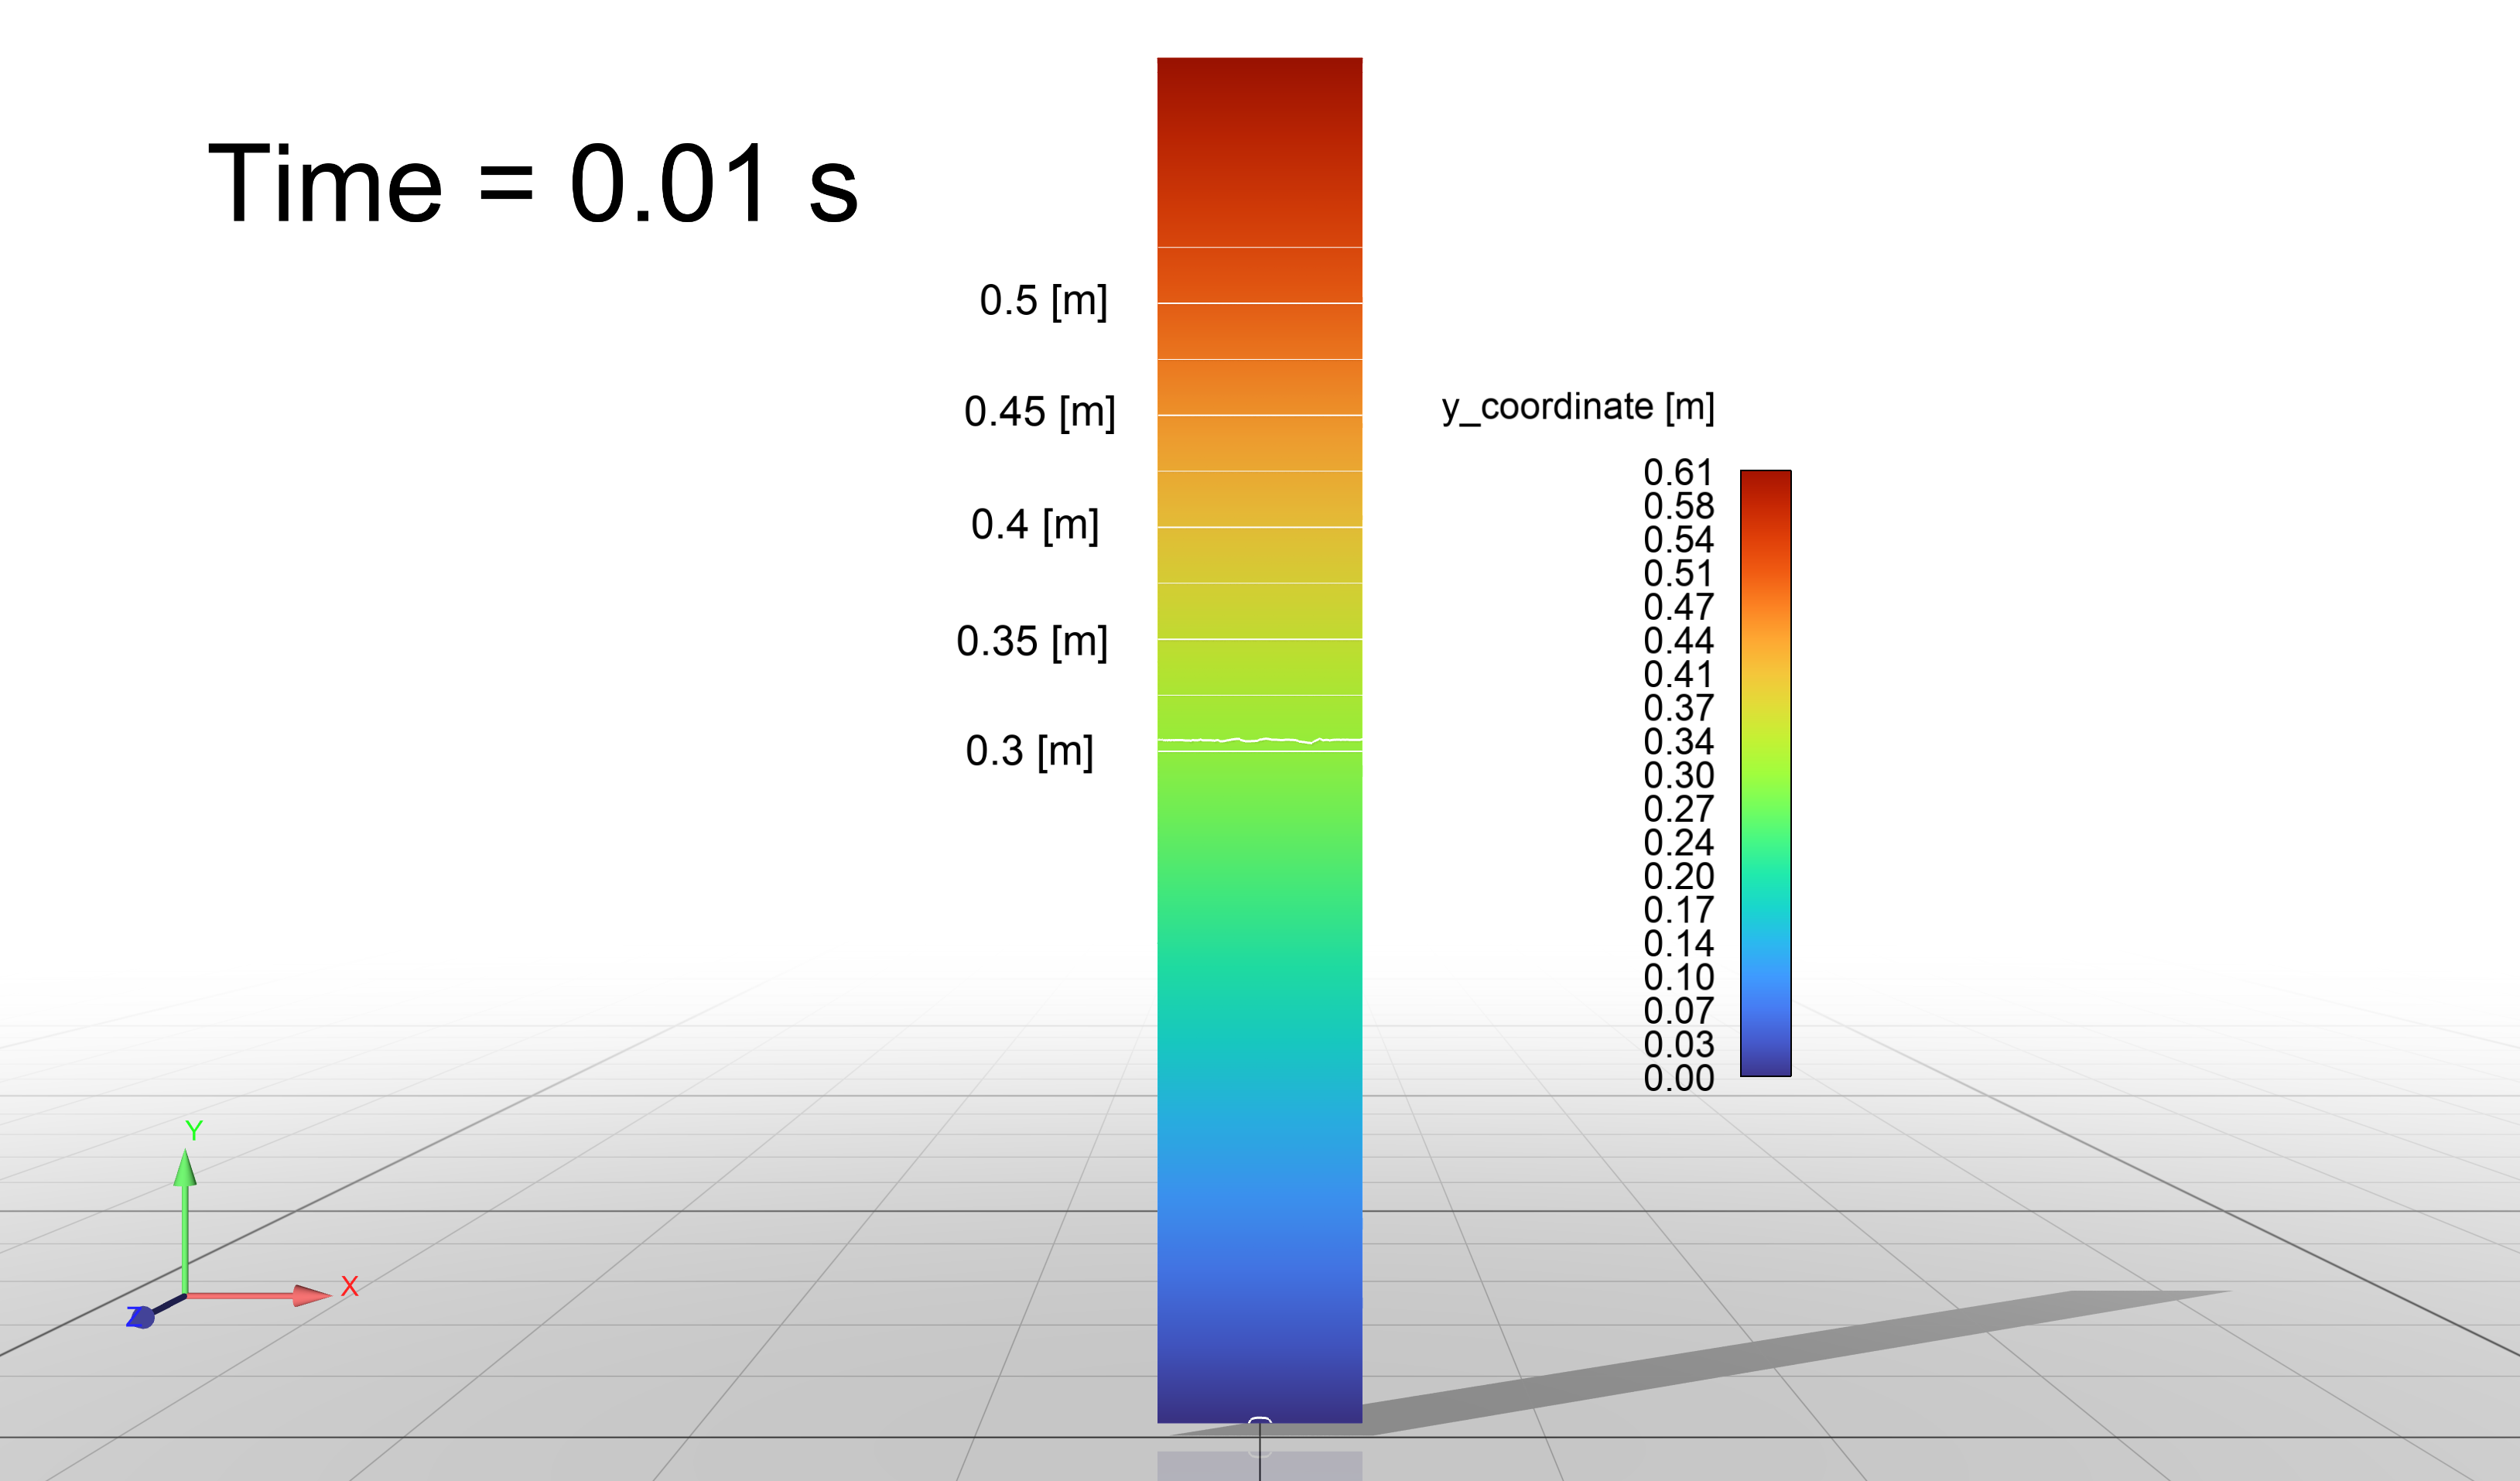
\includegraphics[width=\textwidth]{images/CFD_vapor_inlet_0p01s.png}
\caption{Time = 0.01\,s}
\end{subfigure}

\vspace{1.2em}

\begin{subfigure}[b]{0.95\textwidth}
\centering
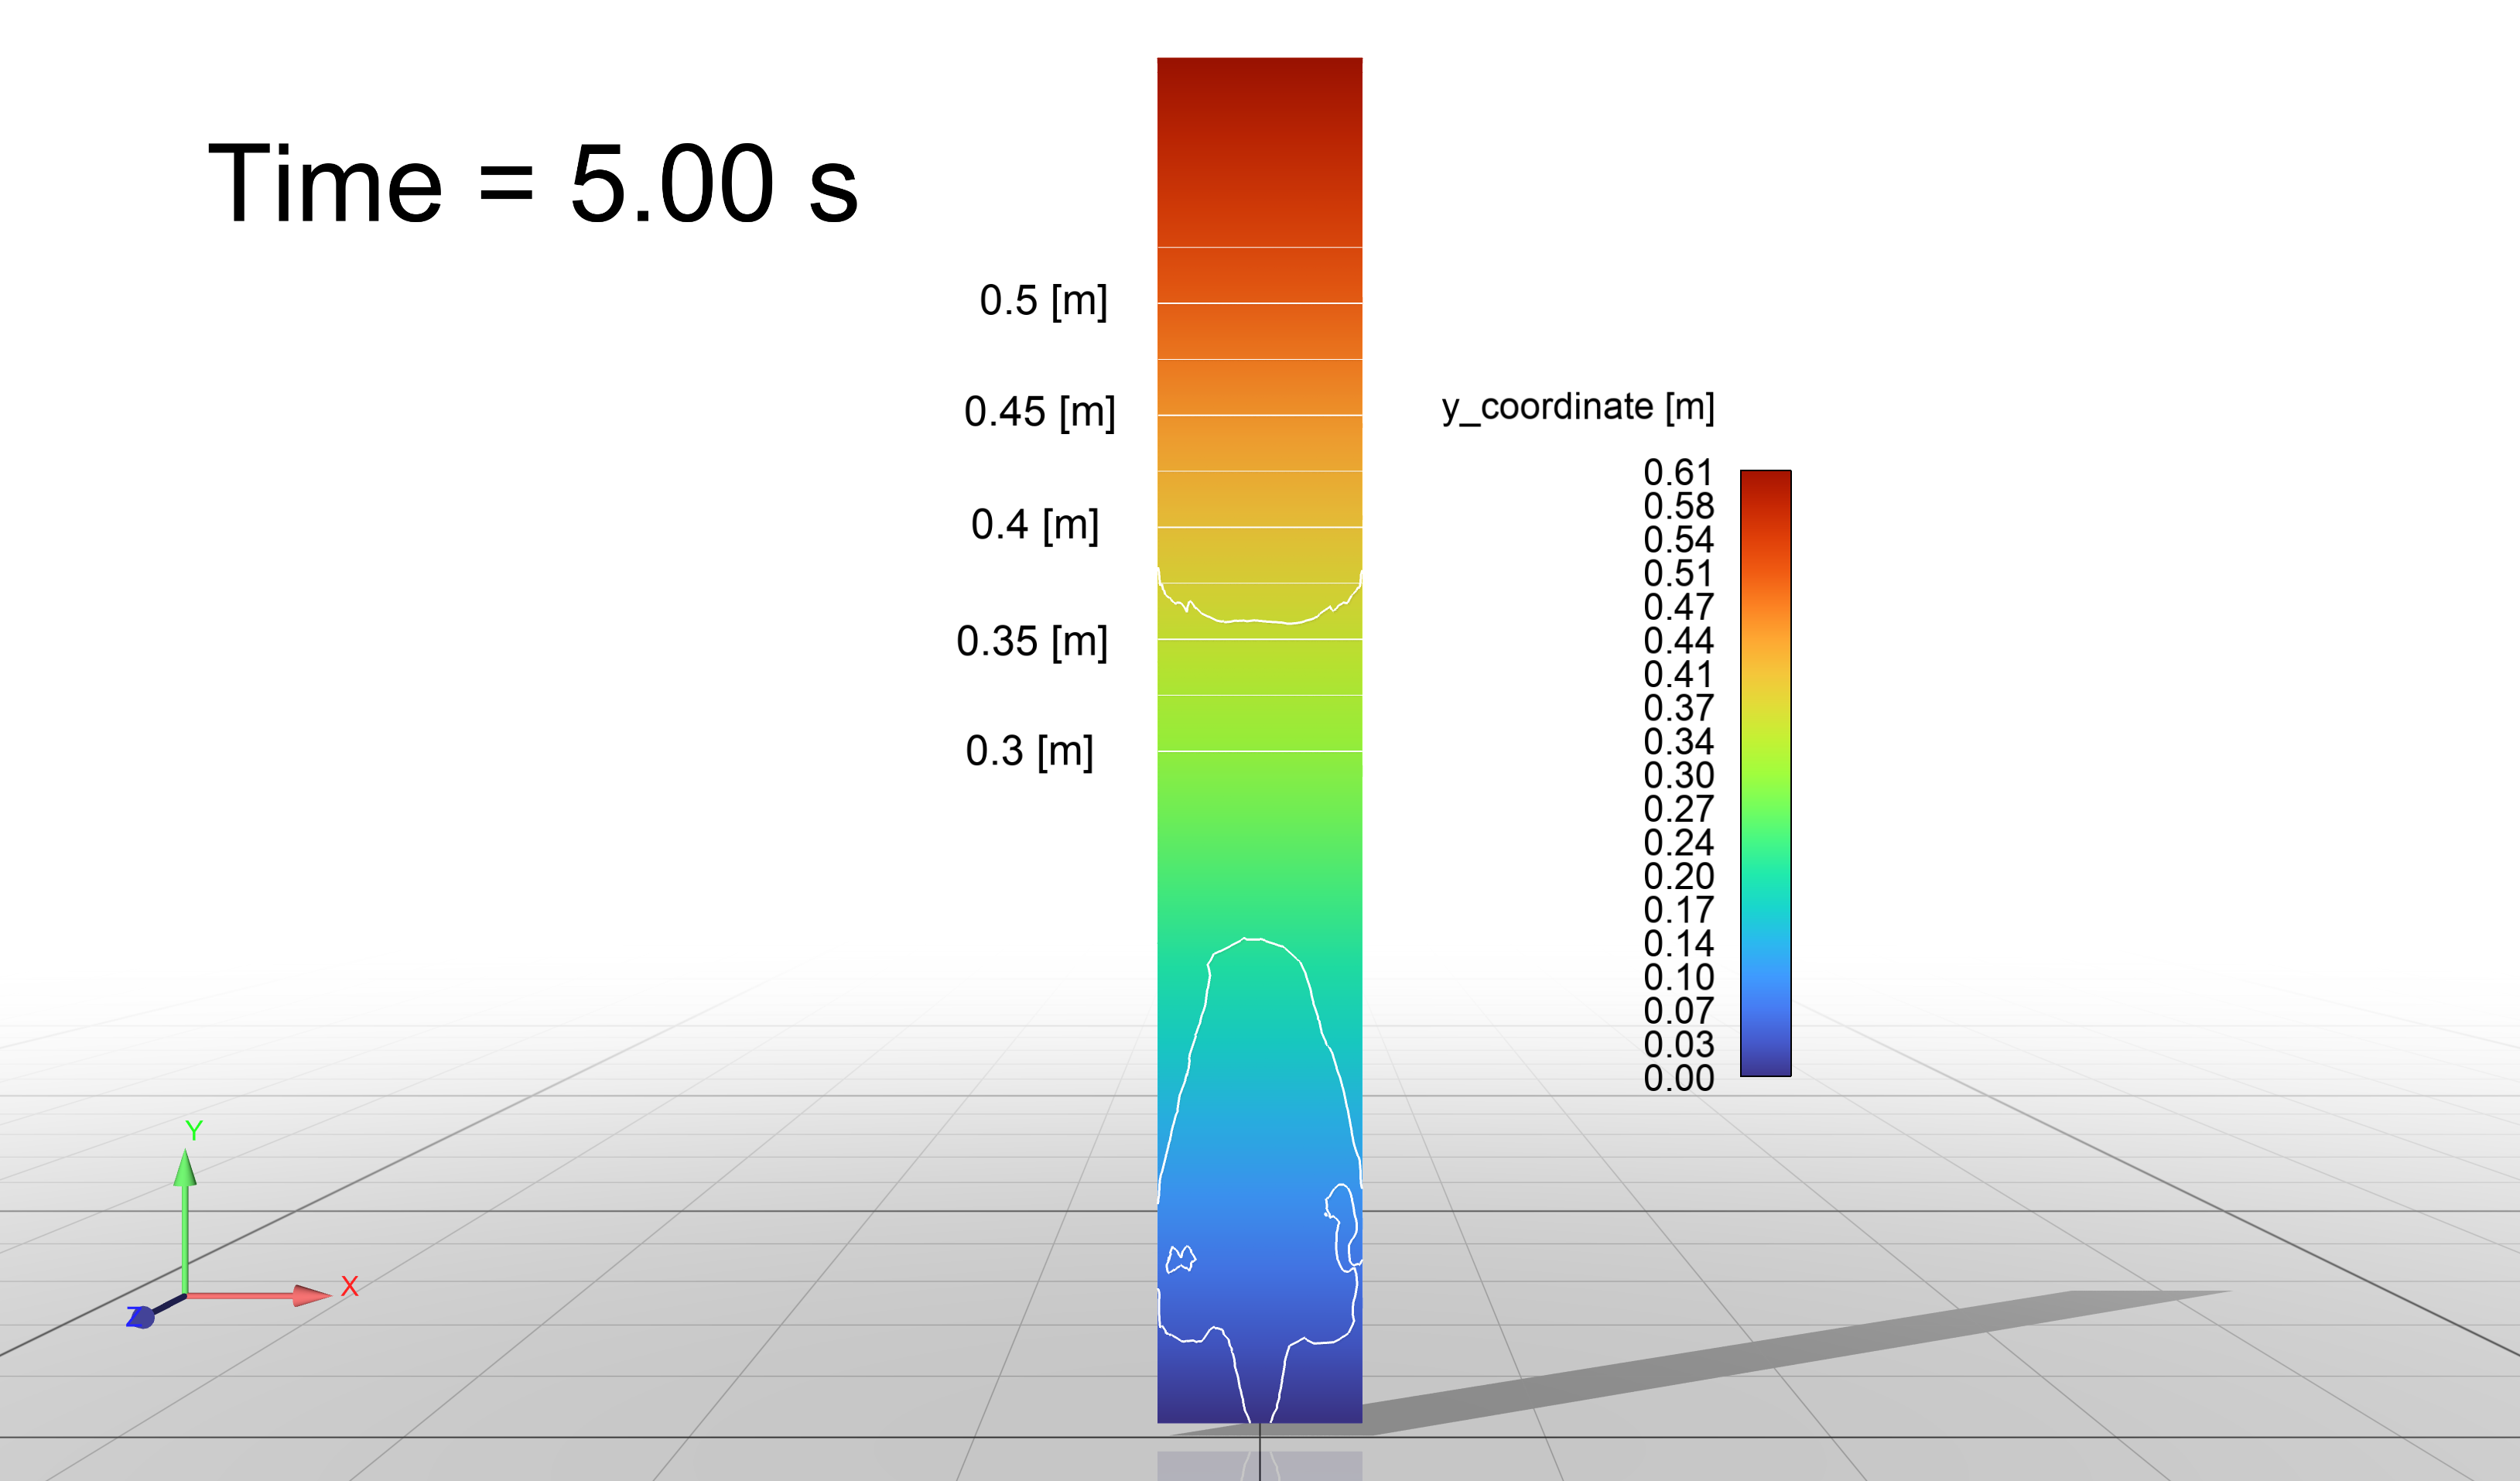
\includegraphics[width=\textwidth]{images/CFD_vapor_inlet_5s.png}
\caption{Time = 5.00\,s}
\end{subfigure}

\caption{CFD visualization of vapor volume fraction (VOF) distribution (blue = liquid, red = vapor) in the 0.3\,ft diameter $\times$ 2.0\,ft height tank at 50\,\% initial fill fraction. The white line represents the VOF = 0.5 isosurface that defines the liquid-vapor interface. A jagged white line marks the primary interface, while a separate white line appears near the bottom due to localized vapor introduction at the orifice. The images illustrate the early vapor injection (top) and the development of wall liquid climb with meniscus curvature by the end of the 5-second simulation (bottom).}
\label{fig:cfd_snapshots}
\end{figure}

Comparison of the liquid-vapor interface height histories demonstrated reasonable quantitative agreement during the early transient phase. The LIQLEV model predicted a maximum bulk liquid level rise of approximately 3.2 inches. In contrast, the 3D CFD simulation yielded a rise of approximately 2.5 inches when measured at the lowest point of the curved meniscus.

The corresponding 3D CFD visualizations of vapor volume fraction at $t=0.01$\,s (top panel) and $t=5.00$\,s (bottom panel) are presented in Figure~\ref{fig:cfd_snapshots}. At early time, vapor has just begun entering from the bottom orifice and the interface remains nearly flat. By $t=5$\,s, significant liquid climb along the tank walls is evident, forming a pronounced curved meniscus (white VOF = 0.5 isosurface). 

Although the lowest point of this curved interface lies approximately 0.5--0.7 inches below the LIQLEV-predicted height, the volume-equivalent (flat-interface) height matches the LIQLEV result closely. This modest discrepancy is physically expected and arises directly from the differing treatment of vapor introduction and interface geometry: LIQLEV assumes spatially uniform vapor addition across the entire tank cross-section, producing idealized piston-like displacement of a flat interface, whereas CFD captures local vapor injection at the orifice and surface-tension-driven meniscus curvature. The close agreement confirms that the LIQLEV framework provides a reliable and conservatively high estimate of bulk liquid displacement driven by boundary-layer boil-off.

This modest discrepancy is physically expected and arises directly from the differing treatment of vapor introduction and interface geometry. In LIQLEV the total boundary-layer vapor volume is treated as a tank-wide scalar and divided by the full cross-sectional area, enforcing idealized piston-like upward displacement of a flat interface. In the CFD domain, vapor enters locally at the bottom orifice, producing a radially spreading velocity field combined with surface-tension-driven meniscus curvature. The lowest point of the three-dimensional interface therefore lies below the volume-equivalent flat-interface height assumed by LIQLEV.

These results confirm that the LIQLEV framework furnishes a reliable and conservatively high estimate of bulk liquid displacement driven by boundary-layer boil-off. This hybrid analytical--CFD approach therefore serves as an effective bridge between rapid parametric scoping with the LIQLEV model and higher-fidelity three-dimensional hydrodynamic validation, substantially strengthening confidence in the LIQLEV predictions.

\subsection{Effect of Tank Size on Meniscus Reorientation Time}

Additional three-dimensional VOF CFD simulations were performed using the same modeling framework (continuum surface force model, high-resolution near-wall prism layers, and SST $k$-$\omega$ turbulence model) to investigate the effect of tank scale on transient liquid-vapor interface reorientation. Two geometries of direct relevance to the experimental matrix were examined: the 0.2\,ft diameter $\times$ 2.0\,ft height Skinner-scale tank and the 6\,cm diameter $\times$ 10\,cm height Labus-scale tank. Each geometry was simulated at three gravity levels ($10^{-3}$\,g, $10^{-4}$\,g, and $10^{-5}$\,g) to quantify the time required for the liquid-vapor interface to reorient from a flat 1$g$ surface to the equilibrium curved meniscus.

The results (Figures~\ref{fig:cfd_meniscus_0p2ft} and \ref{fig:cfd_meniscus_6cm}) reveal two dominant trends. First, meniscus reorientation time increases markedly with decreasing gravity level. Second, the smaller-diameter Labus-scale tank reaches a stable meniscus significantly faster than the 0.2\,ft diameter tank at any given gravity level. These observations are consistent with the reduced Bond number (gravitational-to-surface-tension force ratio) in smaller geometries and lower gravity environments, where surface tension dominates more rapidly.

The CFD-derived meniscus formation times provide important quantitative insight into the pre-venting interface dynamics. For the recommended 0.2--0.3\,ft diameter $\times$ 2.0\,ft height tanks, the simulations indicate that complete reorientation from a flat 1$g$ surface to the equilibrium curved meniscus may require more time than is available before venting would begin in the NASA GRC 5-second zero-gravity facility. Whether full pre-venting meniscus stabilization is actually necessary to meet the scientific objectives remains an open question that will be resolved during the forthcoming physical experiments. Nevertheless, the results confirm that the selected tank scale remains well suited to capture the targeted optically measurable boundary-layer-driven liquid level rise once venting commences.

\begin{figure}[htbp]
\centering
\begin{subfigure}[b]{0.6\textwidth}
\centering
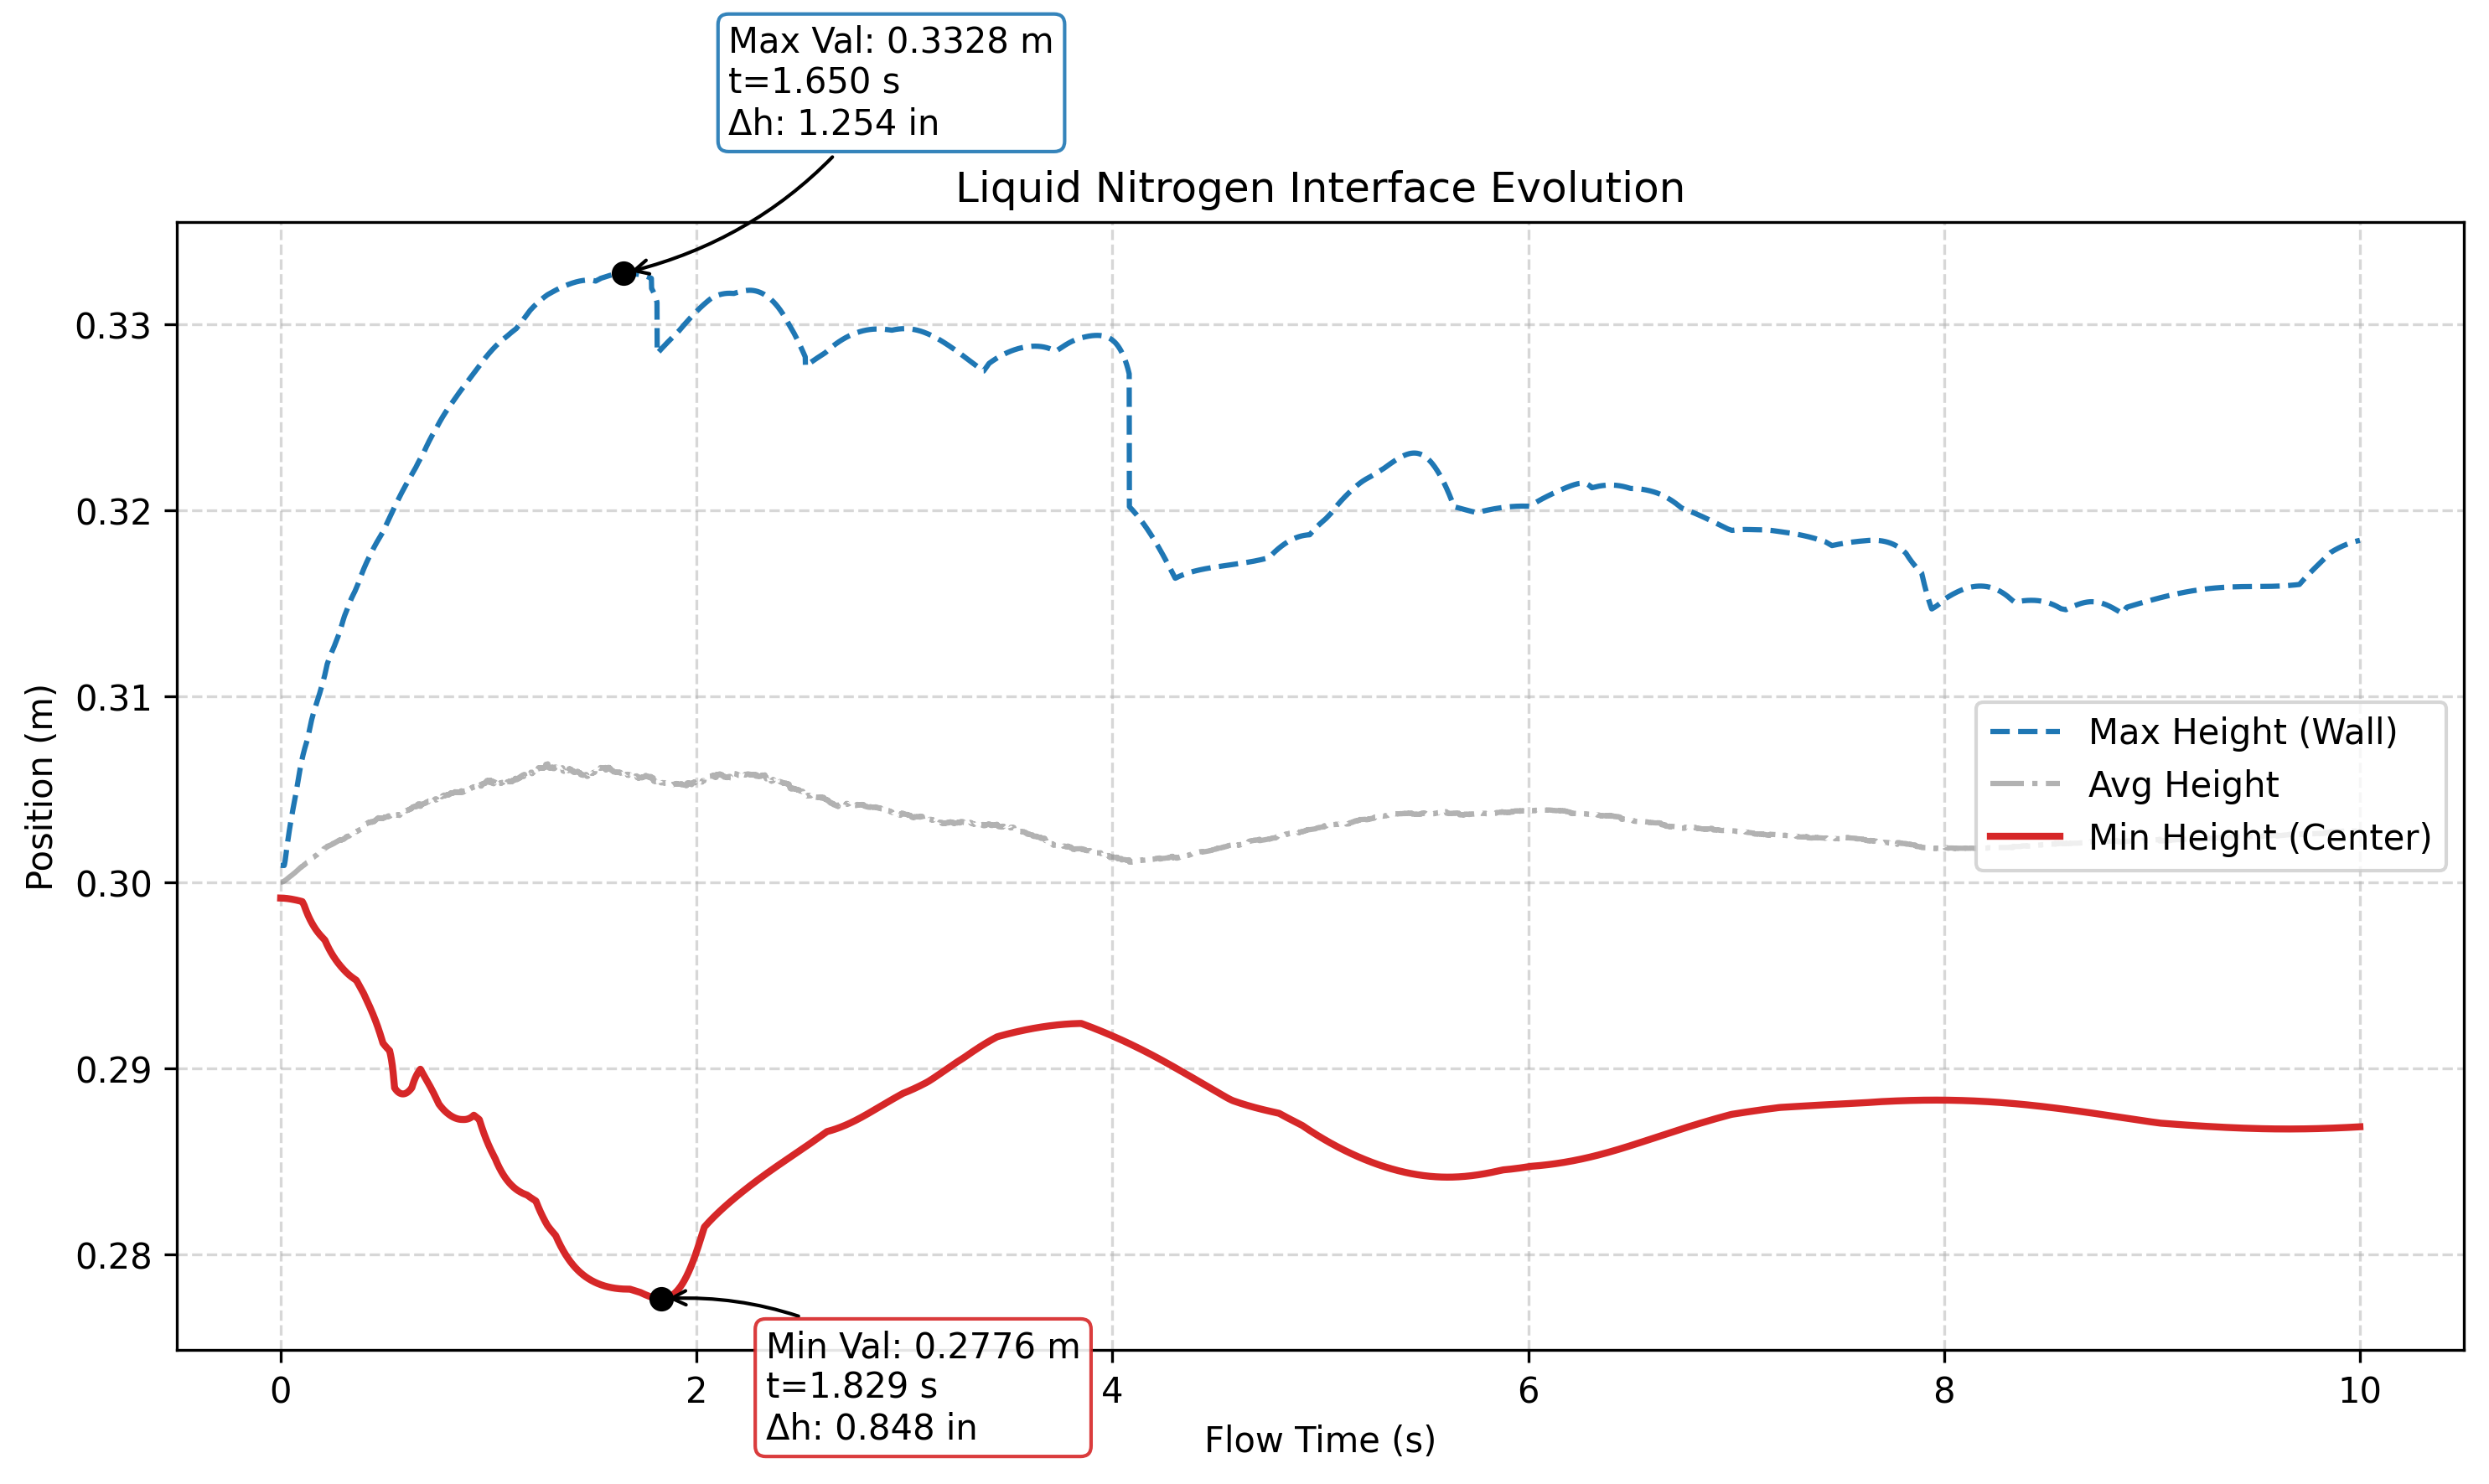
\includegraphics[width=\textwidth]{images/interface_time/cylinder_0p2_1e-3g_redo.png}
\caption{$10^{-3}$\,g}
\end{subfigure}
\vspace{0.6em}

\begin{subfigure}[b]{0.6\textwidth}
\centering
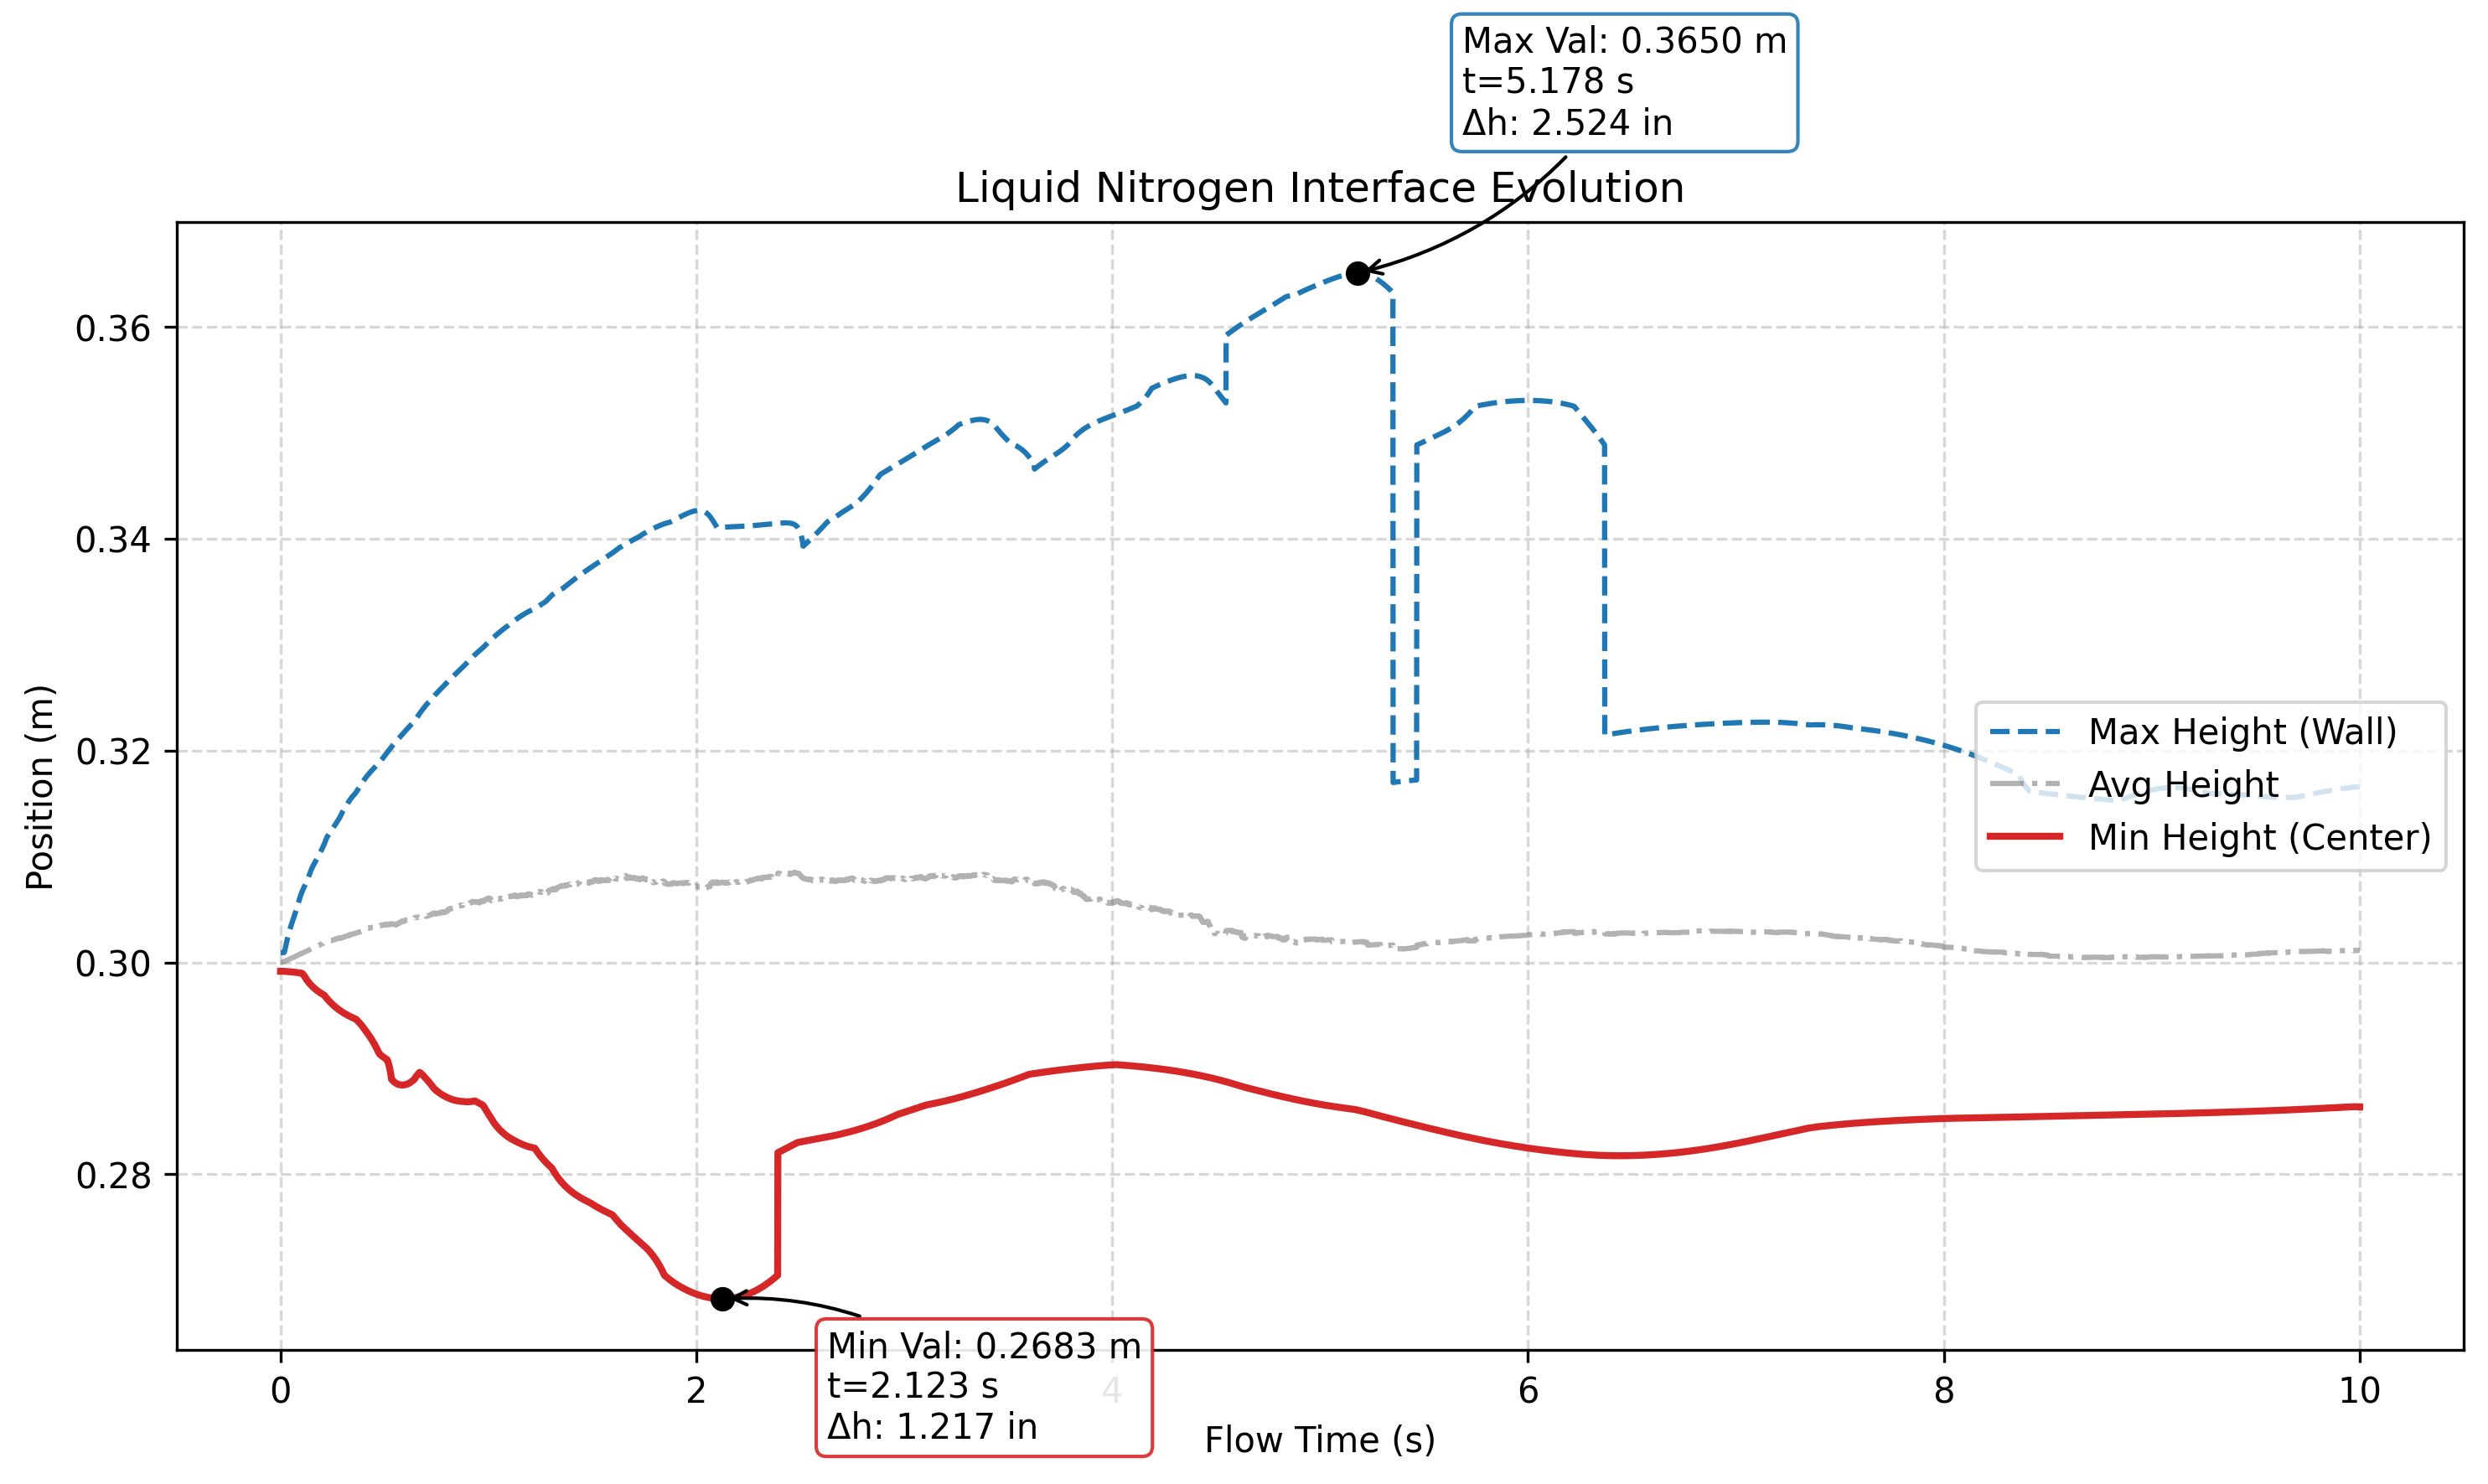
\includegraphics[width=\textwidth]{images/interface_time/cylinder_0p2_1e-4g_redo.png}
\caption{$10^{-4}$\,g}
\end{subfigure}
\vspace{0.6em}

\begin{subfigure}[b]{0.6\textwidth}
\centering
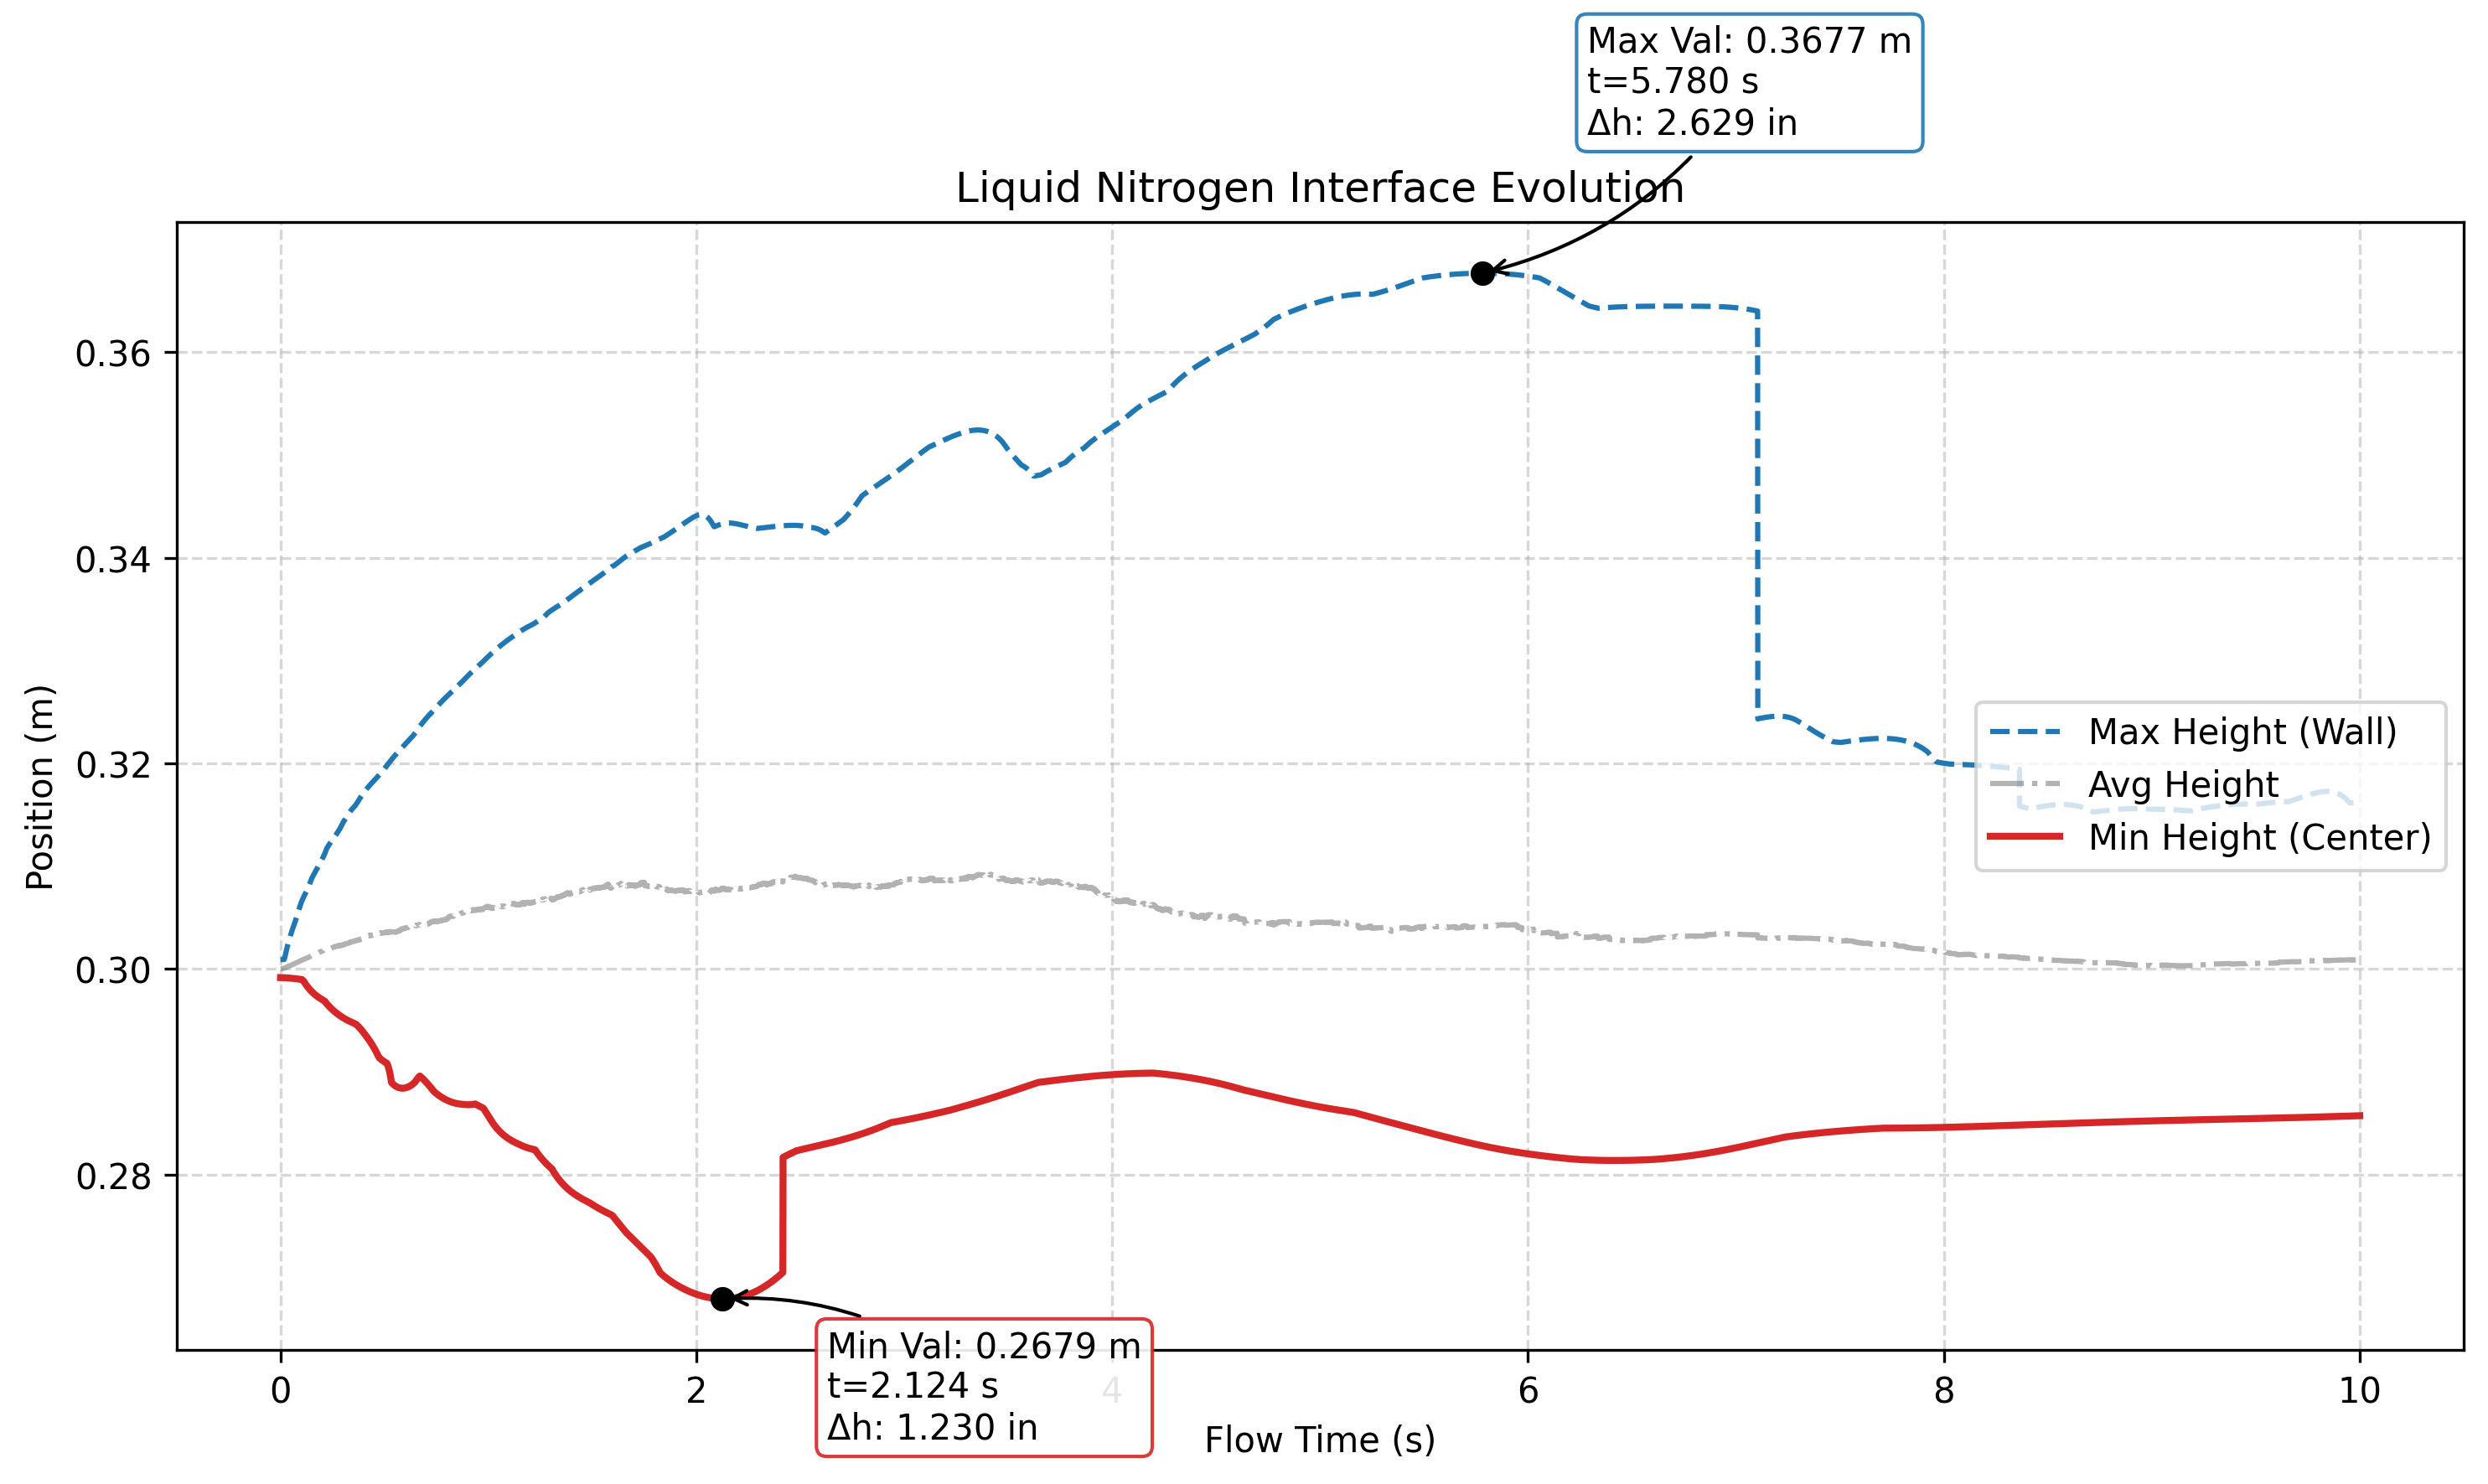
\includegraphics[width=\textwidth]{images/interface_time/cylinder_0p2_1e-5g_redo.png}
\caption{$10^{-5}$\,g}
\end{subfigure}
\caption{Liquid nitrogen interface evolution for the 0.2\,ft diameter $\times$ 2\,ft height tank at three gravity levels. Blue: maximum height at wall; gray: average height; red: minimum height at center. Lower gravity substantially delays meniscus reorientation.}
\label{fig:cfd_meniscus_0p2ft}
\end{figure}

\begin{figure}[htbp]
\centering
\begin{subfigure}[b]{0.6\textwidth}
\centering
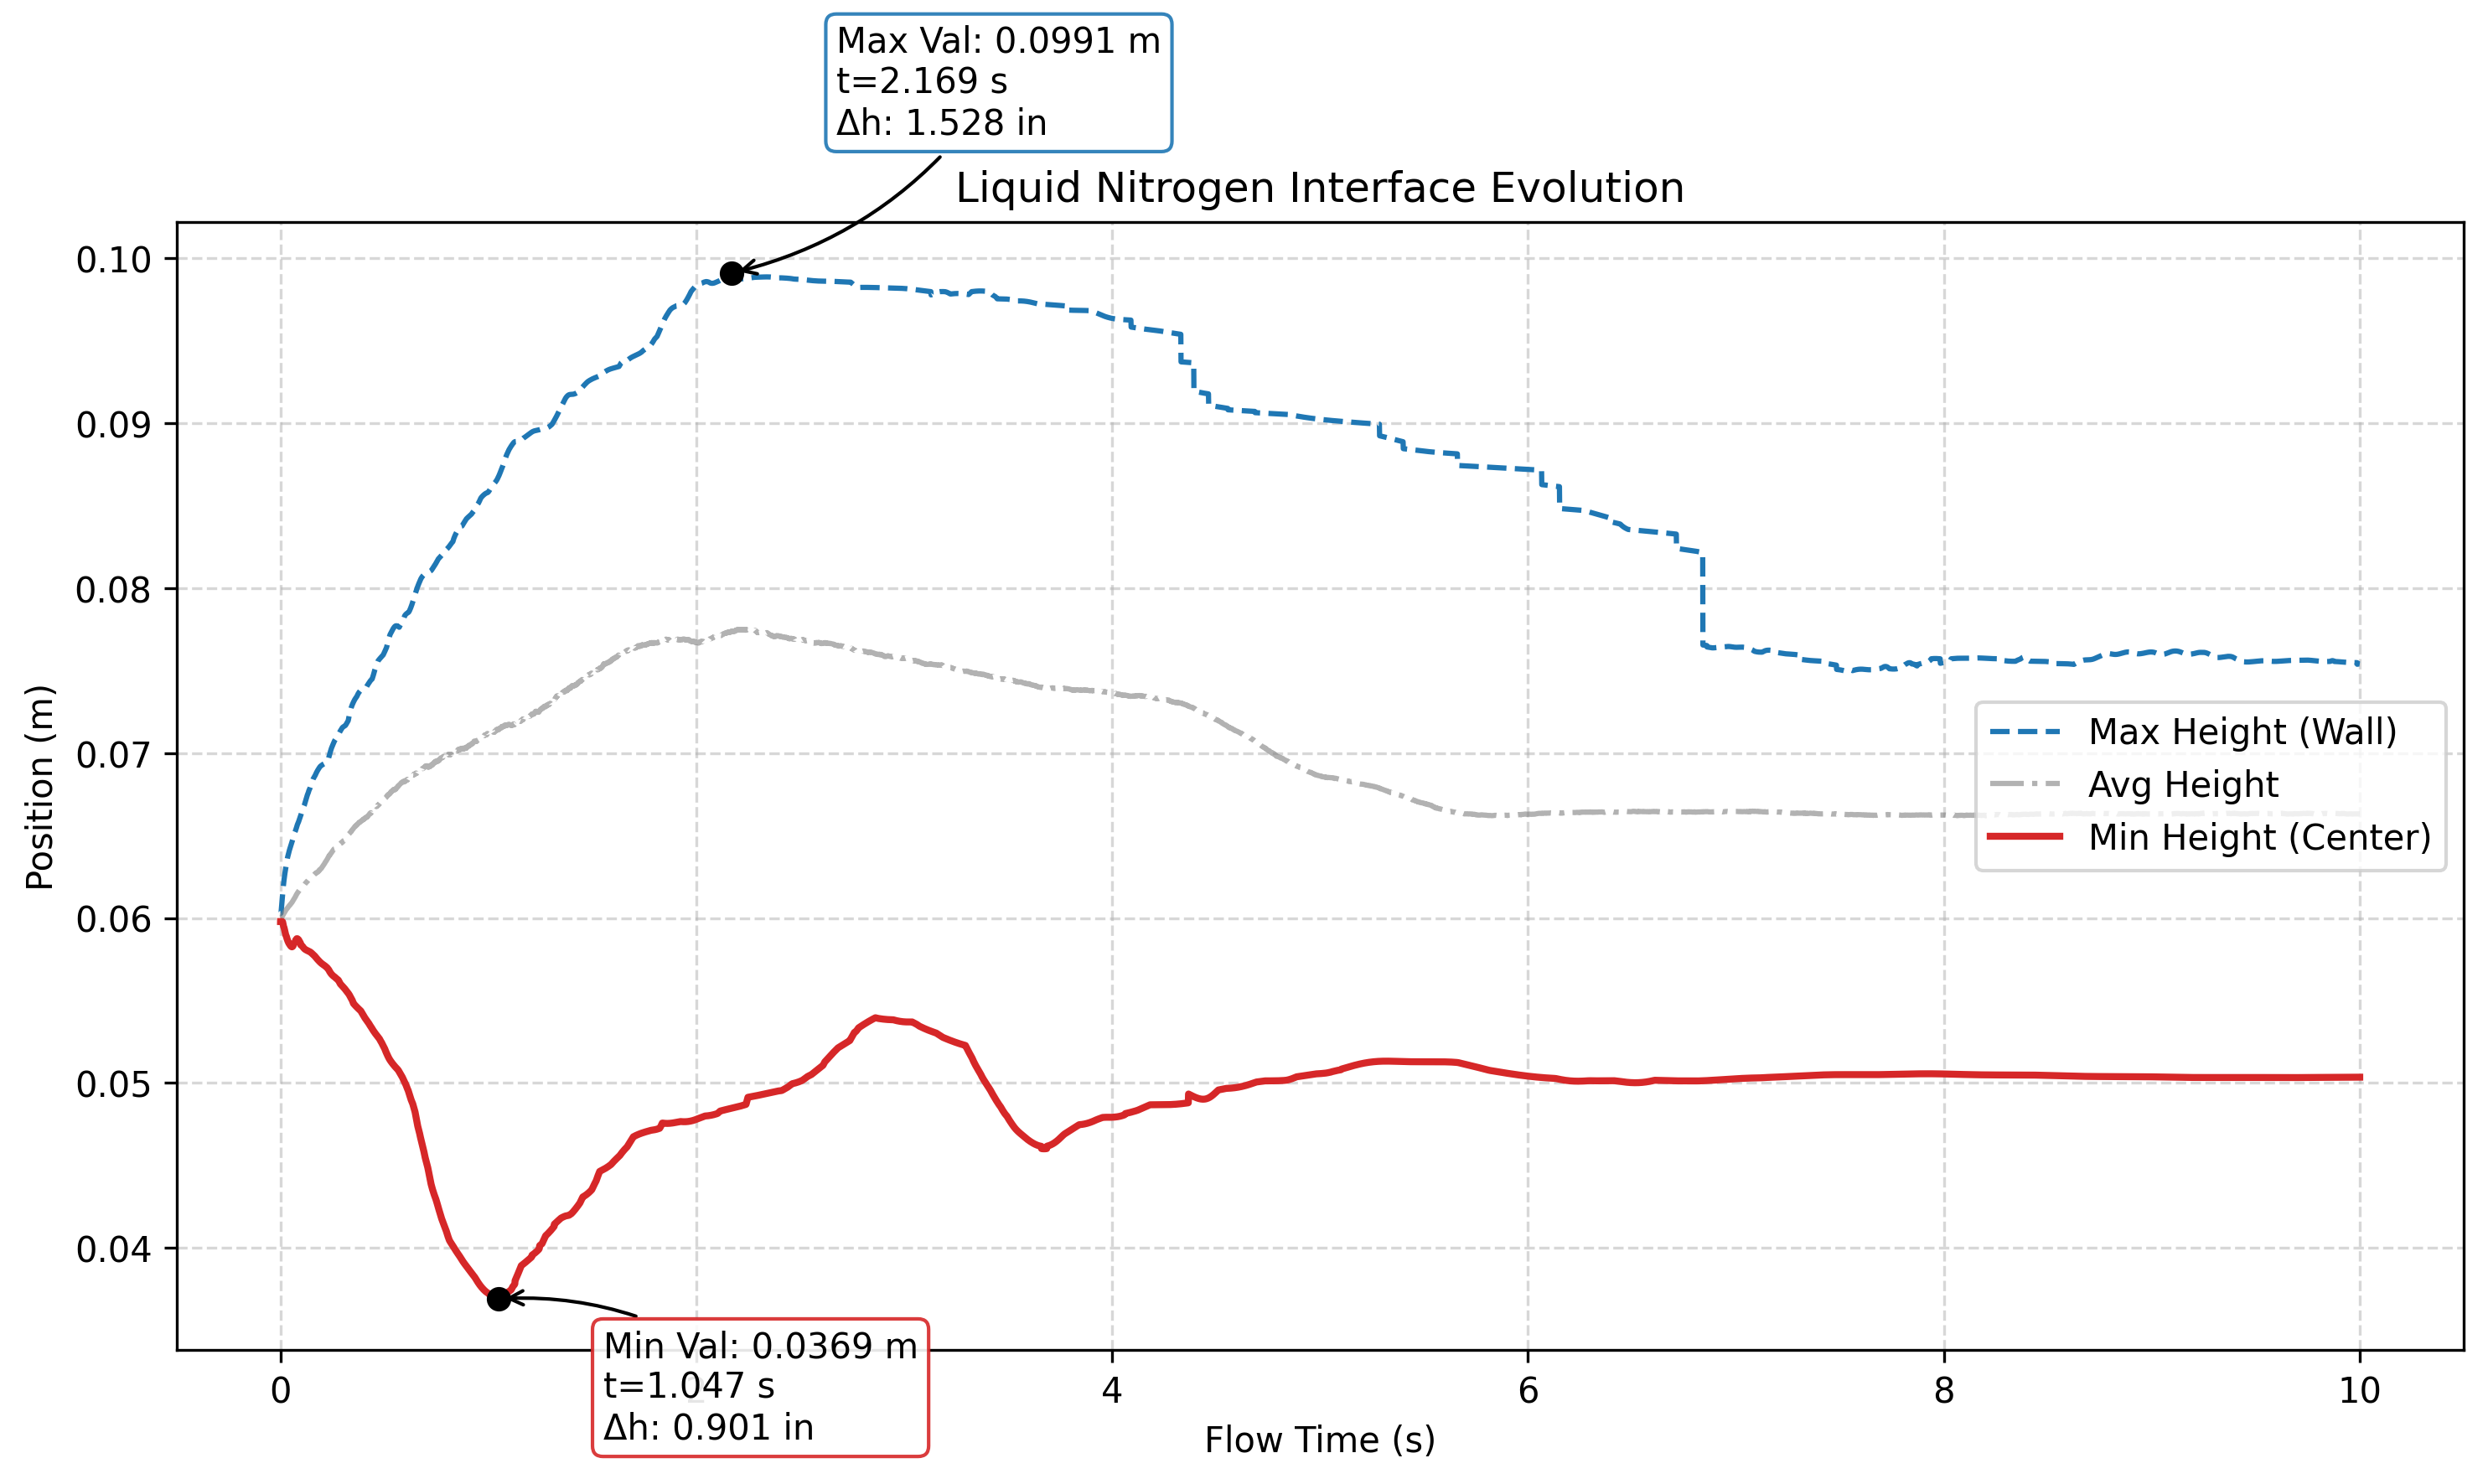
\includegraphics[width=\textwidth]{images/interface_time/cylinder_6cm_1e-3g_redo.png}
\caption{$10^{-3}$\,g}
\end{subfigure}
\vspace{0.6em}

\begin{subfigure}[b]{0.6\textwidth}
\centering
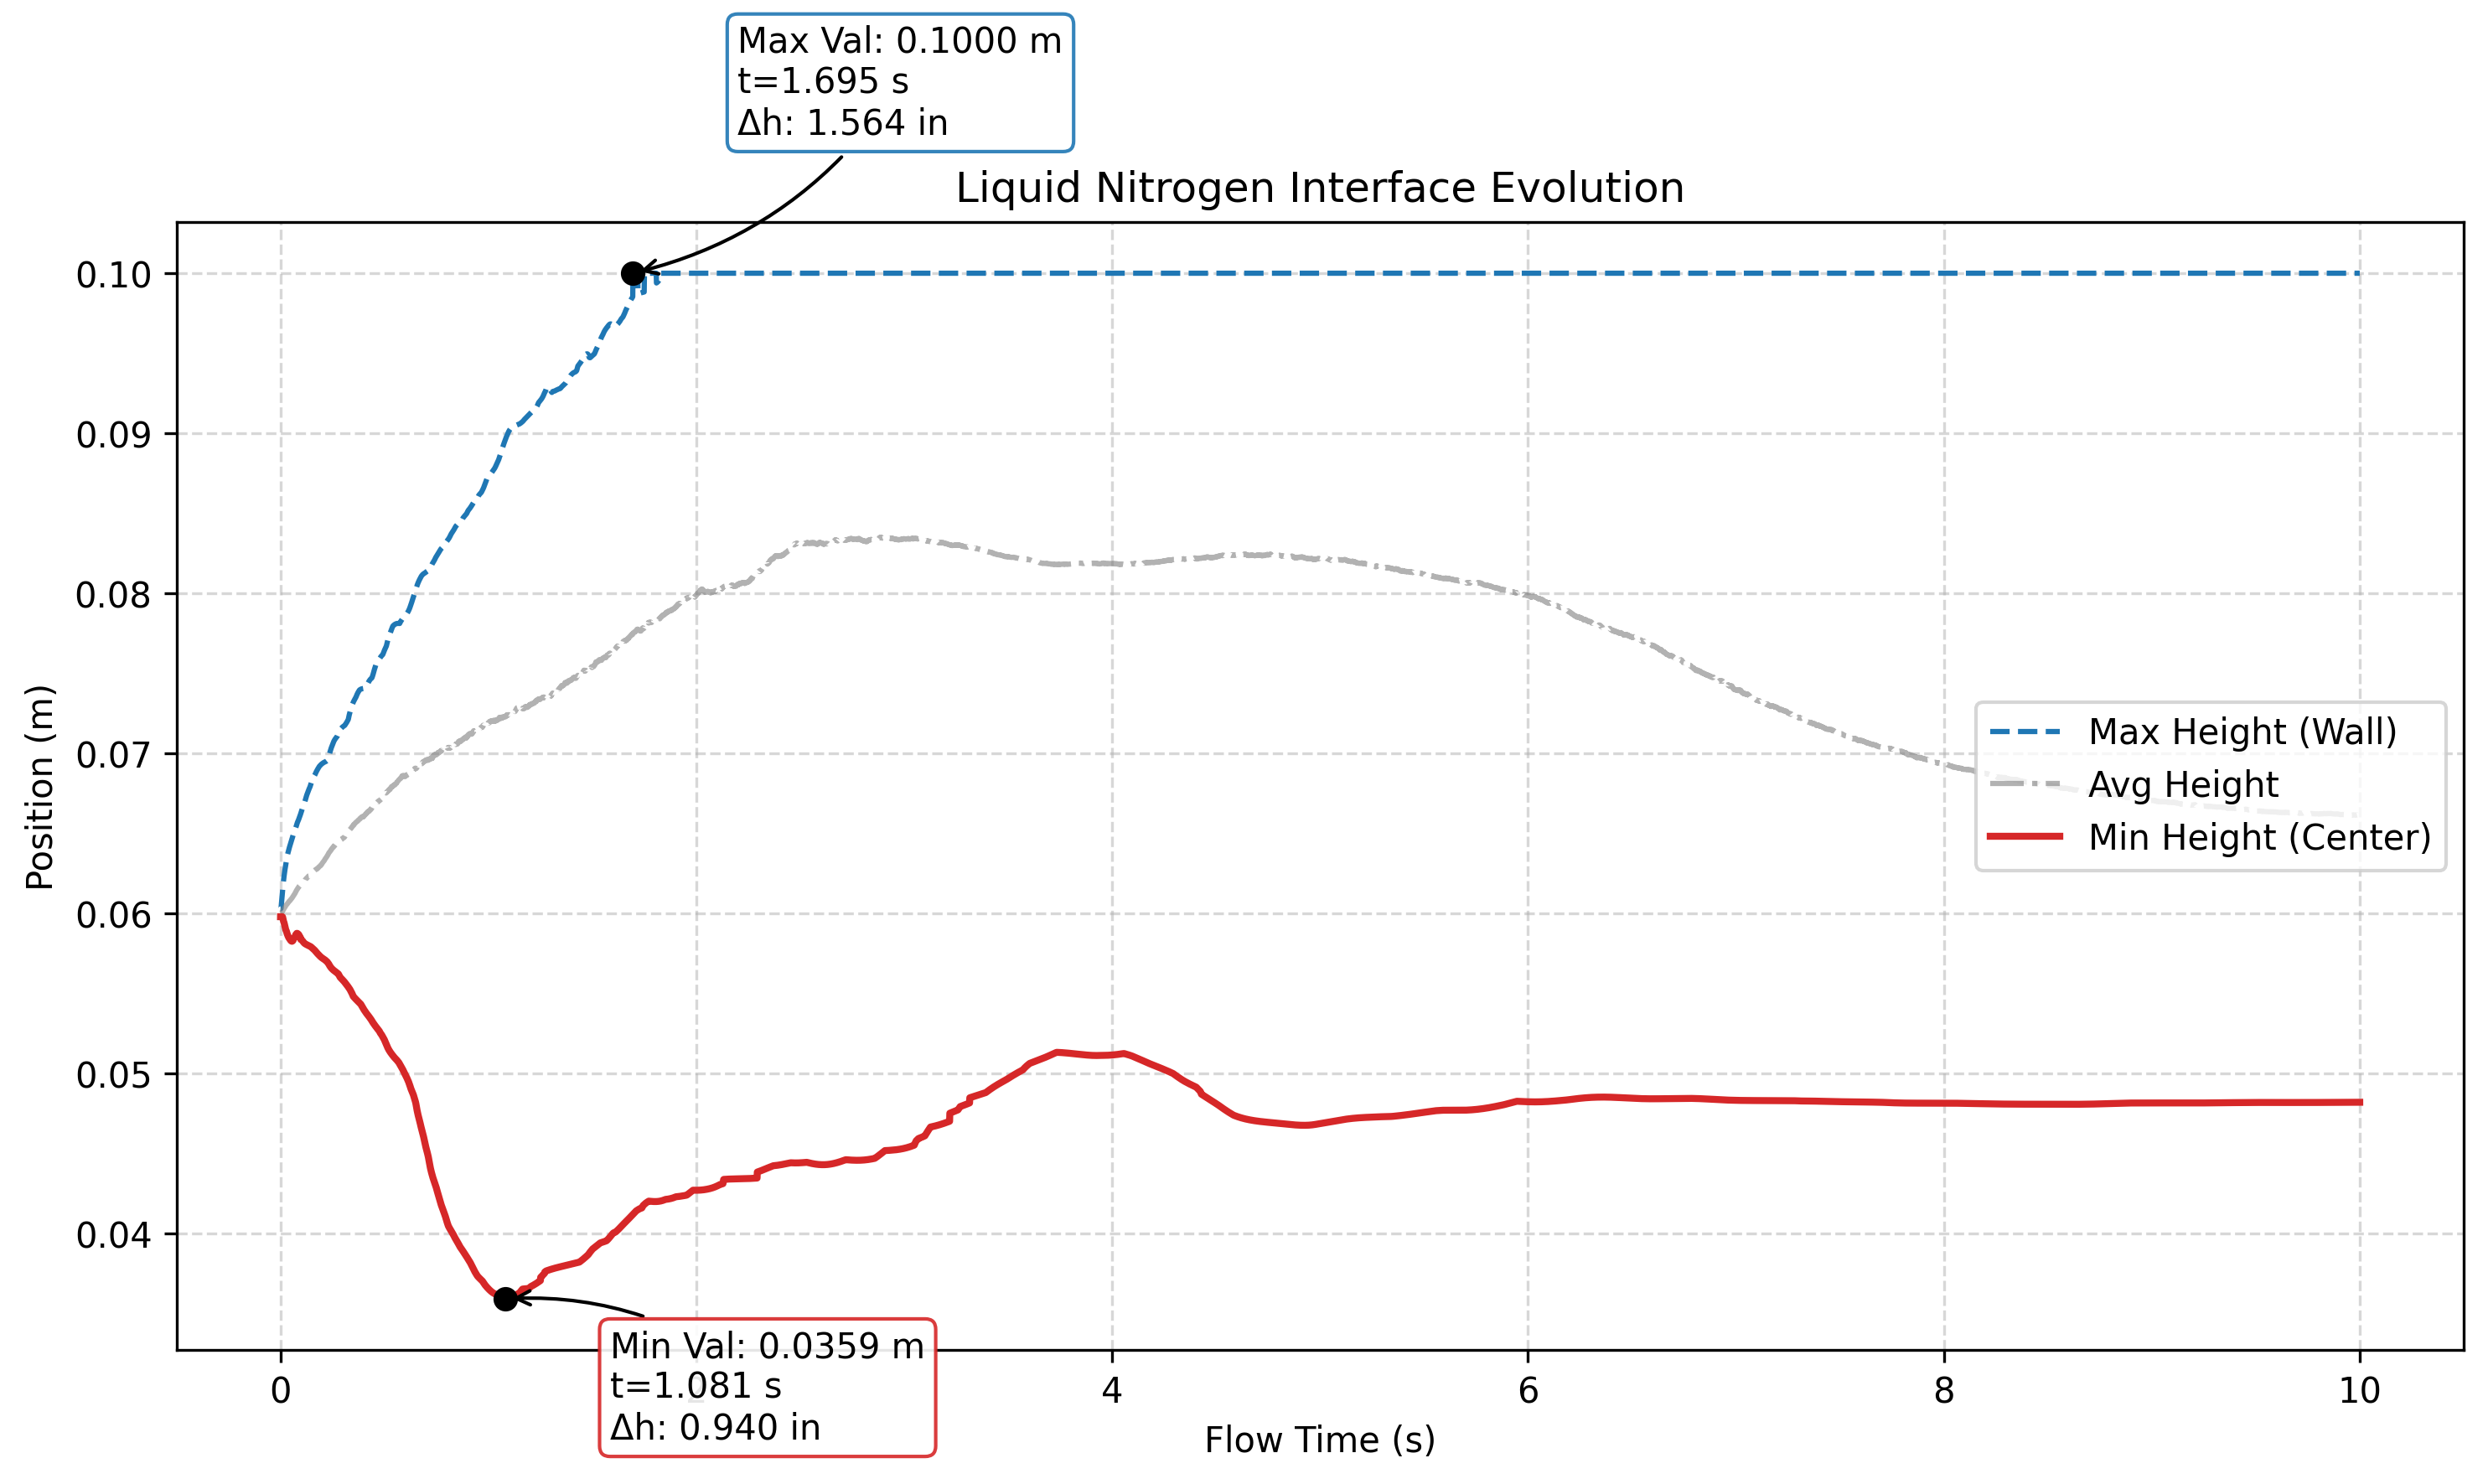
\includegraphics[width=\textwidth]{images/interface_time/cylinder_6cm_1e-4g_redo.png}
\caption{$10^{-4}$\,g}
\end{subfigure}
\vspace{0.6em}

\begin{subfigure}[b]{0.6\textwidth}
\centering
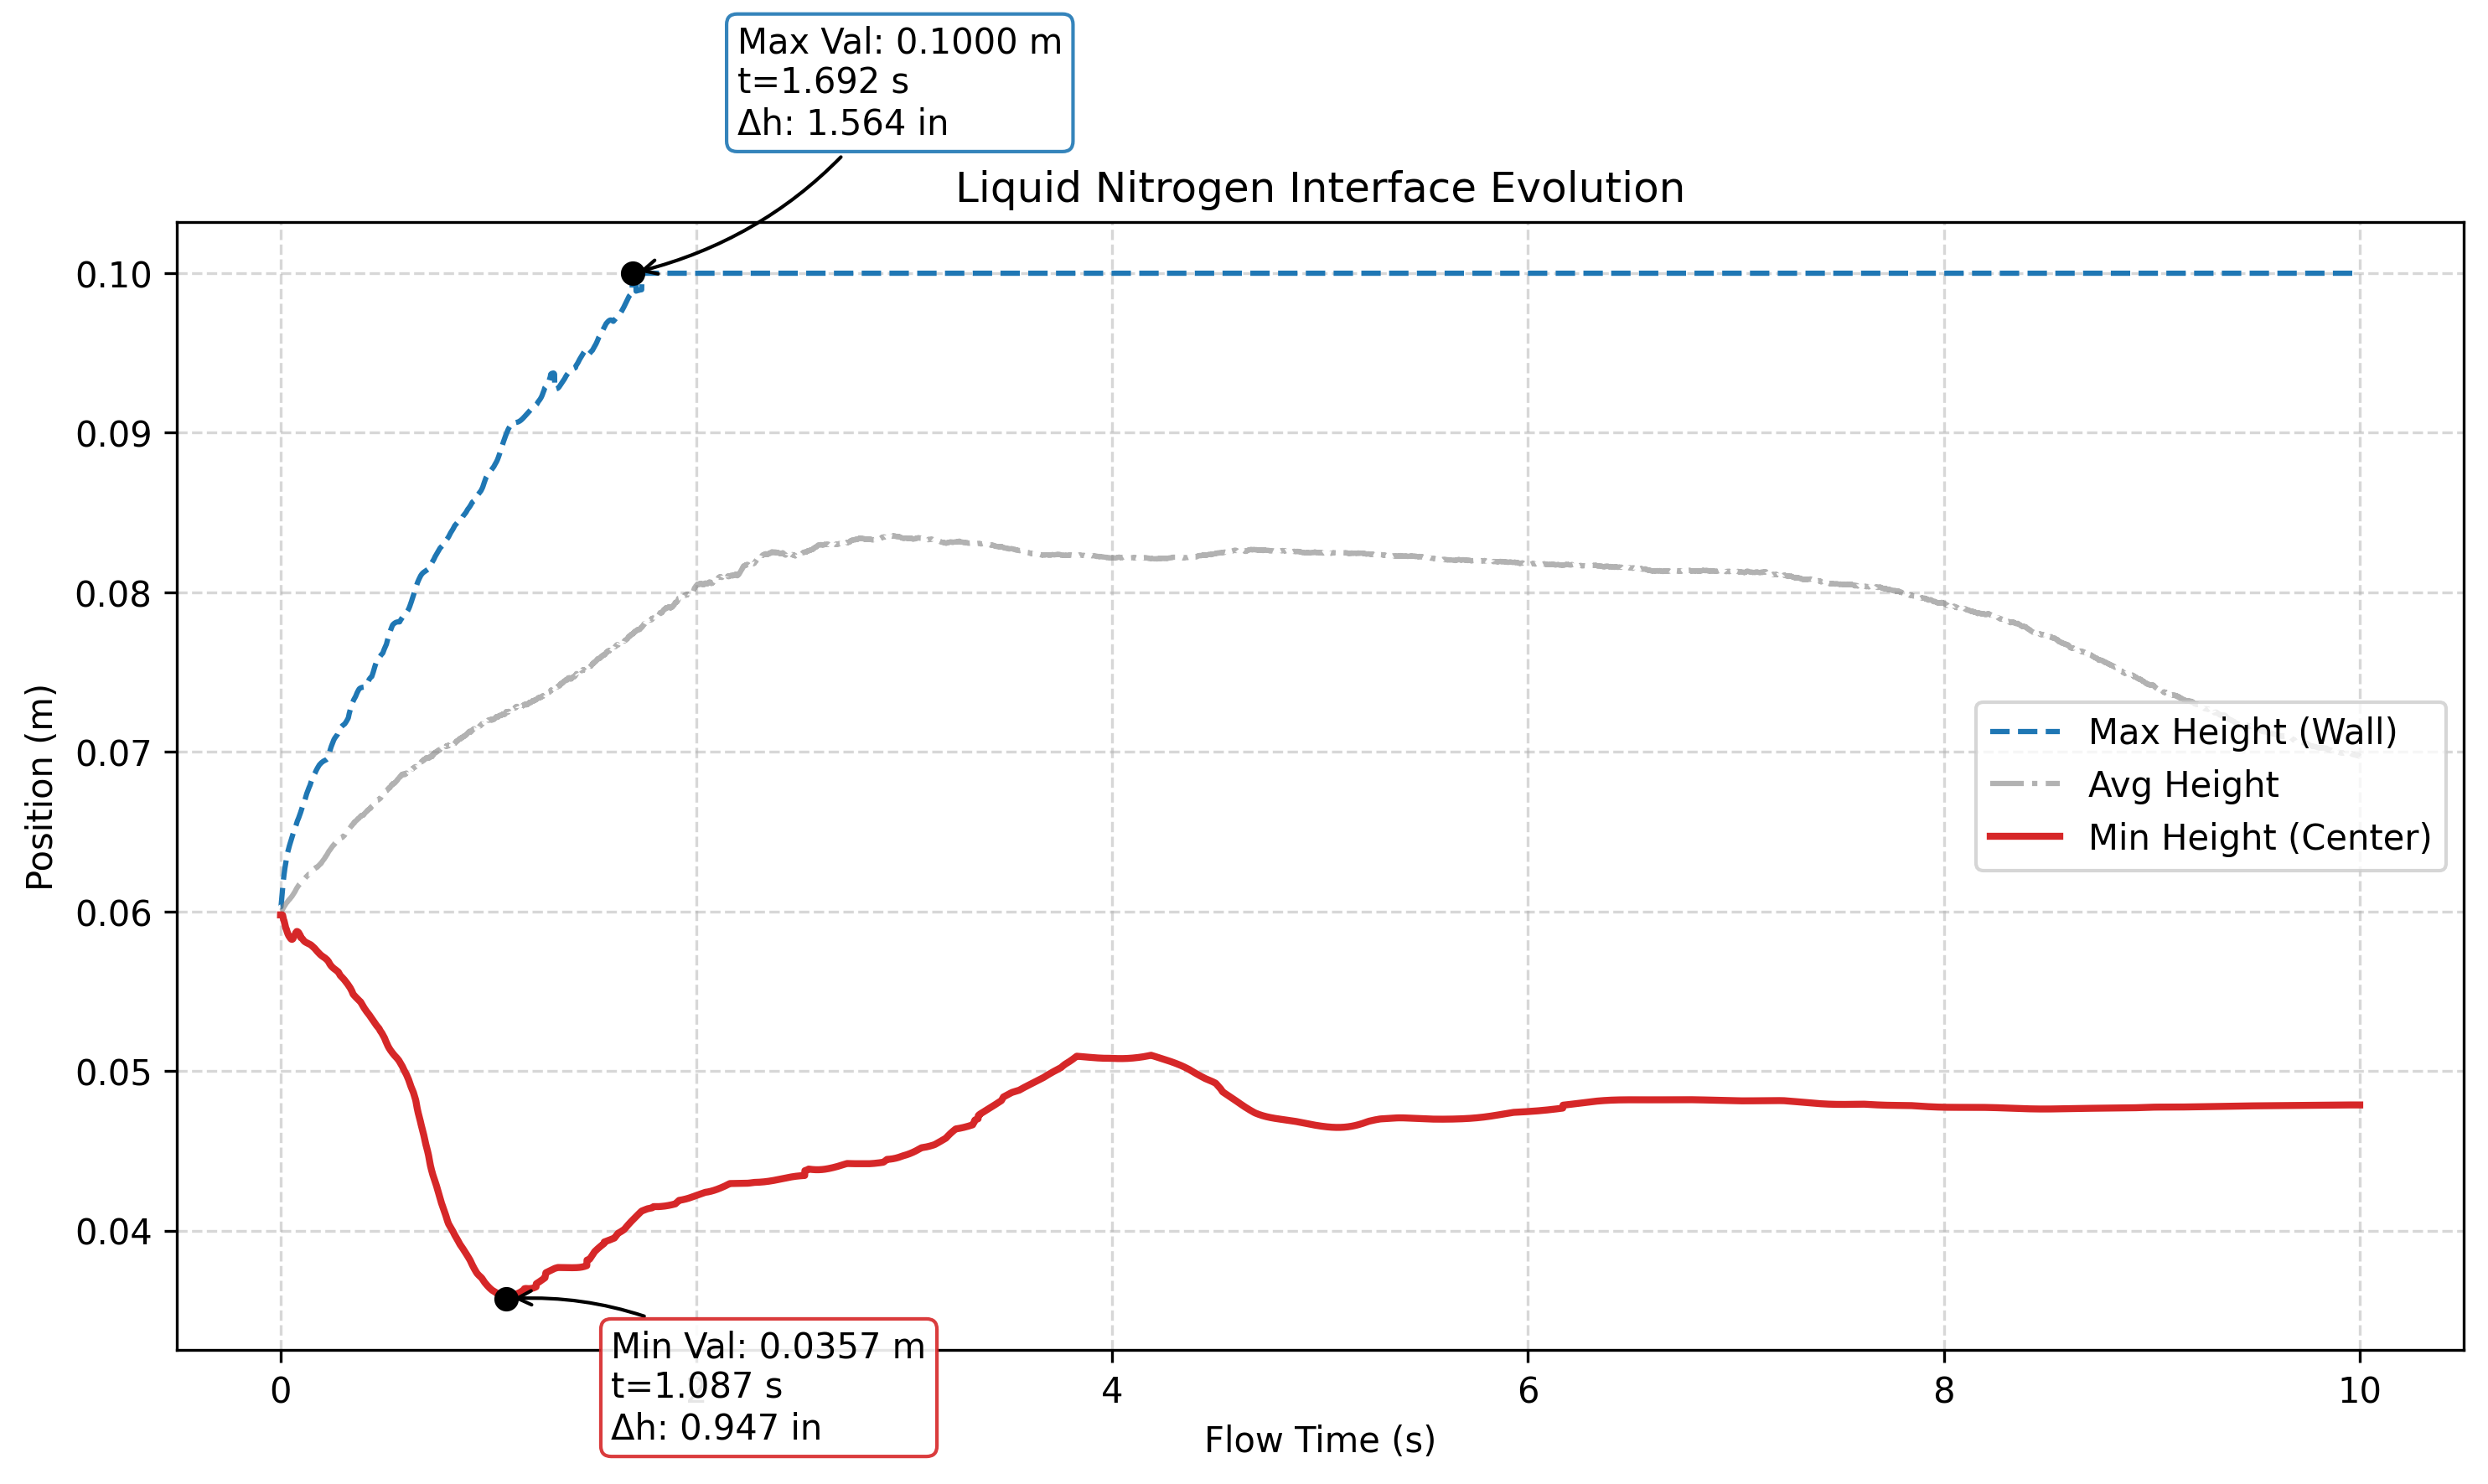
\includegraphics[width=\textwidth]{images/interface_time/cylinder_6cm_1e-5g_redo.png}
\caption{$10^{-5}$\,g}
\end{subfigure}
\caption{Liquid nitrogen interface evolution for the 6\,cm diameter $\times$ 10\,cm height tank at three gravity levels. The smaller tank scale results in faster meniscus stabilization compared with the 0.2\,ft tank at equivalent gravity.}
\label{fig:cfd_meniscus_6cm}
\end{figure}


\section{Conclusions and Recommendations}
The modernization of the legacy LIQLEV boundary-layer model into a robust, multiprocessing Python framework integrated with CoolProp represents a major advancement in the predictive analysis of zero-gravity venting and transient liquid level rise. The enhanced thermodynamic fidelity, flexible vent-profile handling, dynamic $\epsilon$ modeling, and efficient parametric-sweep capability now enable high-accuracy evaluations across a wide range of propellants, tank scales, and reduced-gravity environments.

Based on the comprehensive parametric studies performed to fulfill the FY25 Drop Tower LLR Study, the following recommendations are made for the forthcoming reduced-gravity experiments:

\begin{enumerate}
    \item \textbf{NASA GRC 5-Second Zero-Gravity Facility:} This platform provides the optimal balance of true high-quality microgravity ($\sim10^{-5}$\,g) and sufficient test duration for the full development of wall boundary-layer boil-off and attainment of the peak thermodynamic liquid level rise. Recommended test articles are small-diameter cylindrical tanks (0.3\,ft diameter $\times$ 2.0\,ft height, $L/D\approx6.67$) using Nitrogen as the working fluid. Initial fill fractions should be maintained between 40\% and 65\% with moderate constant vent rates (0.003--0.006\,lbm/s). Under these optimized conditions, the peak interface rise is typically attained between 3.5 and 4.8\,s, well within the available window and without lid impingement, delivering clean, high-value optical data suitable for CFD correlation.
    
    \item \textbf{NASA GRC 2.2-Second Drop Tower:} This facility is generally too short to capture the maximum thermodynamic liquid level rise. Even with high fill fractions ($\sim$75--80\,\%) and aggressive vent rates, only the early transient phase of boundary-layer vapor generation can be observed before many configurations reach lid impingement. It is best reserved for studying the initial depressurization response.
    
    \item \textbf{Parabolic Flight Campaigns:} These were ultimately not pursued. Although the model indicated that at least 3 inches of rise could be achieved during the low-g plateau, persistent lateral acceleration components ($\sim10^{-2}$ to $5\times10^{-3}$\,g) inherent to the parabolic maneuver excite unidirectional sloshing that would contaminate the boundary-layer-driven interface dynamics. This limitation was confirmed through transient CFD simulations incorporating full three-axis flight profiles and by independent parabolic-slosh experiments reported in the literature.
    
    \item \textbf{CFD Correlation Development:} The verified LIQLEV macro-scale results, including the JAXA-validated bulk-boiling augmentation ($\epsilon\approx50$ for large tanks), provide well-characterized boundary conditions and precise timelines for liquid-vapor interface evolution. These data should be used to anchor higher-fidelity multiphase VOF CFD simulations, substantially reducing the required temporal domain and enabling detailed correlation of local boiling, bubble dynamics, and interface motion.
\end{enumerate}

The optimized experimental configurations and modeling insights developed in this study will ensure that the planned physical testing yields high-quality, directly usable data. These results will directly support the refinement of vent-system models and improve cryogenic fluid management capabilities for future long-duration spaceflight missions. Future development should incorporate an explicit bulk-liquid boiling source term alongside the original wall boundary-layer formulation, providing a physically complete model that retains the computational efficiency of the current framework across all tank scales. The Python implementation (liqlev\_simulation and liqlev\_sweep.py) and all parametric sweep results are available from the authors upon request.

\section*{Acknowledgment}

The authors acknowledge the VBA adaptations developed by Matt Moran, which provided the essential foundation for this effort.

\bibliography{references}

\end{document}